\documentclass[parskip=full]{scrartcl}
\usepackage[T1]{fontenc}    % avoid garbled Unicode text in pdf
\usepackage[utf8]{inputenc} % use utf8 file encoding for TeX sources
\usepackage[german]{babel}  % german hyphenation, quotes, etc
\usepackage{hyperref}       % detailed hyperlink/pdf configuration
\hypersetup{                % ‘texdoc hyperref‘ for options
pdftitle={PSE: Entwicklung eines relationalen Debuggers - Pflichtenheft},%
,%
}
\usepackage{graphicx}       % provides commands for including figures
\usepackage{csquotes}       % provides \enquote{} macro for "quotes"
\usepackage[nonumberlist]{glossaries}     % provides glossary commands
\usepackage{enumitem}
\usepackage{xcolor}
\usepackage{lscape}
\newcommand\frage[1]{\textcolor{red}{#1}}


\font\myfont=cmr12 at 16pt

\title{
	\vspace{2cm}
	\myfont 
	Praxis der Softwareentwicklung:\\ 
	Entwicklung eines relationalen Debuggers\\
}
\subtitle{
	\vspace{1cm}
	\myfont
	Entwurfsdokument
}
\author{
	\vspace{1cm} \\
	Benedikt Wagner\\
	\texttt{udpto@student.kit.edu}
	\and \vspace{1cm} \\ Chiara Staudenmaier\\
	\texttt{uzhtd@student.kit.edu}
	\and Etienne Brunner\\
	\texttt{urmlp@student.kit.edu}
	\and Joana Plewnia\\
	\texttt{uhfpm@student.kit.edu} 
	\and Pascal Zwick\\
	\texttt{uyqpk@student.kit.edu}
	\and Ulla Scheler\\
	\texttt{ujuhe@student.kit.edu}
	\vspace{1cm}
	\and Betreuer: Mihai Herda, Michael Kirsten
	\vspace{4cm}
}


\begin{document}
\clearpage
\maketitle
\pagenumbering{gobble}
\newpage

\tableofcontents
\newpage
\pagenumbering{arabic}
%Eventuell Fußnoten generieren
\section{Einleitung}
%Einleitung mit grobem Überblick. Dieser Abschnitt soll an das Pflichtenheft anschließen.
Dieses Dokument dokumentiert die Ergebnisse der Entwurfsphase (\textit{28.11.-22.12.2017}) im Rahmen des Moduls Praxis der Softwareentwicklung (PSE) am Lehrstuhl \enquote{Anwendungsorientierte formale Verifikation - Prof. Dr. Beckert} am Karlsruher Institut für Technologie (KIT).\\
Hierbei handelt es sich um den Entwurf des Produkts \textit{DIbugger}, das im Pflichtenheft definiert wurde. Aufgabe des \textit{DIbuggers} ist es, dem Nutzer zu helfen, mehrere Programme gleichzeitig zu debuggen und interaktiv zu analysieren. \\
Dabei wurde in den Anforderungskriterien unter anderem festgelgt, dass neben Konzepten eines herkömmlichen Debuggers wie Einzelschritten und Breakpoints, auch zusätzliche  Konzepte enthalten sein sollen, die den Umgang mit zwei oder mehr Programmläufen erleichtern. Beispiel für ein solches Konzept sind die Watch-Expressions, bei denen der Nutzer Zusammenhänge zwischen Variablen aus verschiedenen Programmen untersuchen kann. So soll das Finden relationaler Eigenschaften unterstützt werden. \\
Dieses Dokument erläutert nun, wie diese Anforderungen softwaretechnisch umgesetzt werden sollen. Dazu wird zunächst ein Überblick über den Aufbau des gesamten Projektes gegeben (Kapitel \ref{Übersicht} und \ref{GlobalePatterns}) und dann die einzelnen Pakete, inklusive ihrer wichtigsten Klassen, erklärt (Kapitel \ref{UI}, \ref{Control}, \ref{FileHandler} und \ref{DebugLogic}). Für einen genaueren Einblick, wie die Pakete zusammenarbeiten, empfiehlt sich Kapitel \ref{charAbl} über charakteristische Abläufe. Kapitel \ref{implementierung} stellt den Zeitplan für die Implementierungsphase (\textit{09.01.-02.02.2018}) vor. Die restlichen Kapitel befassen sich mit Spezifika des Entwurfs.

%Das Entwurfsdokument beschreibt die Paketeinteilung, Beschreibung der Klassen und Abläufe und genaue Spezifikation der Abhängigkeiten und Kernkomponenten. 
%\\Die Implementierung während der Implementierungsphase (\textit{09.01.-02.02.2018}) wird anhand der Vorgaben in diesem Dokument durchgeführt. \\
%Hierbei werden die aus der Softwaretechnik bekannten Prinzipien, wie etwa Geheimnisprinzip und Kapselungsprizip oder das Prinzip der losen Kopplung berücksichtigt. Wie genau die Einhaltung der Prinzipien sichergestellt wird, wird an den jeweiligen Stellen im Dokument erwähnt. 
\vspace{1cm}
\begin{figure}[!h]
\centering

\includegraphics[width=0.8\textwidth]{../Plichtenheft/logo_nongi.png}
\caption{Produktlogo}
\end{figure}

\newpage
\section{Übersicht}
\label{Übersicht}
\begin{figure}[!h]
\centering
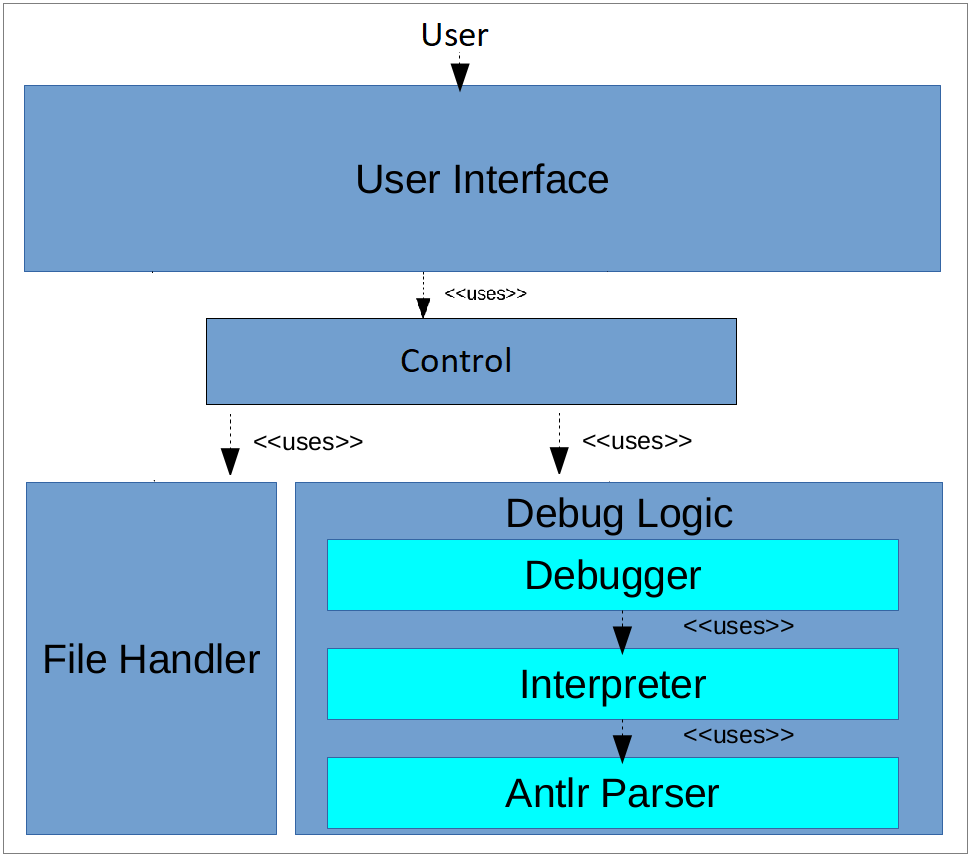
\includegraphics[width=0.5\textwidth]{../Plichtenheft/Architektur.png} \\
\caption{Architekturdiagramm}
\label{Architekturdiagramm}
\end{figure}
Das Produkt ist aufgeteilt in die vier Pakete \textit{Control}, \textit{UserInterface}, \textit{FileHandler} und \textit{DebugLogic}. 
Dabei hat jedes Paket seine eigene Aufgabe:
\begin{itemize}
\item Das \textit{UserInterface} beinhaltet den Code für die Benutzeroberfläche, also alles, was der Nutzer vom Produkt sieht.
\item Die \textit{Control} nimmt die Benutzereingaben entgegen und steuert die Interaktion zwischen dem \textit{UserInterface} und der \textit{DebugLogic}.
\item Die \textit{DebugLogic} enthält die Anwendungslogik.
\item Der \textit{FileHandler} ist dazu da, Daten zu speichern und zu lesen.
\end{itemize}

Möchte der Nutzer beispielsweise mit dem Debuggen beginnen und drückt den entsprechenden Knopf auf der Benutzeroberfläche, setzt die \textit{Control} diesen Befehl um, indem sie die notwendigen Schritte der \textit{DebugLogic} ausführt. Will der Nutzer seine Ergebnisse später speichern, drückt er wieder einen Knopf auf der Benutzeroberfläche und der Befehl wird wieder vom \textit{UserInterface} an die \textit{Control} weitergegeben, die dieses Mal zum Speichern den \textit{FileHandler} aufruft. In Abbildung \ref{Architekturdiagramm} sind die Pakete und die Benutztrelation dargestellt. \\
Aus der Abbildung wird ebenfalls ersichtlich, dass die \textit{DebugLogic} aus den Unterpaketen \textit{Debugger}, \textit{Interpreter} und \textit{AntlrParser} besteht. Deren Funktionalität wird in Kapitel \ref{DebugLogic} dargelegt. \\



\newpage
\section{Global genutzte Entwurfsmuster}
\label{GlobalePatterns}
\begin{figure}[!h]
\makebox[\textwidth][c]{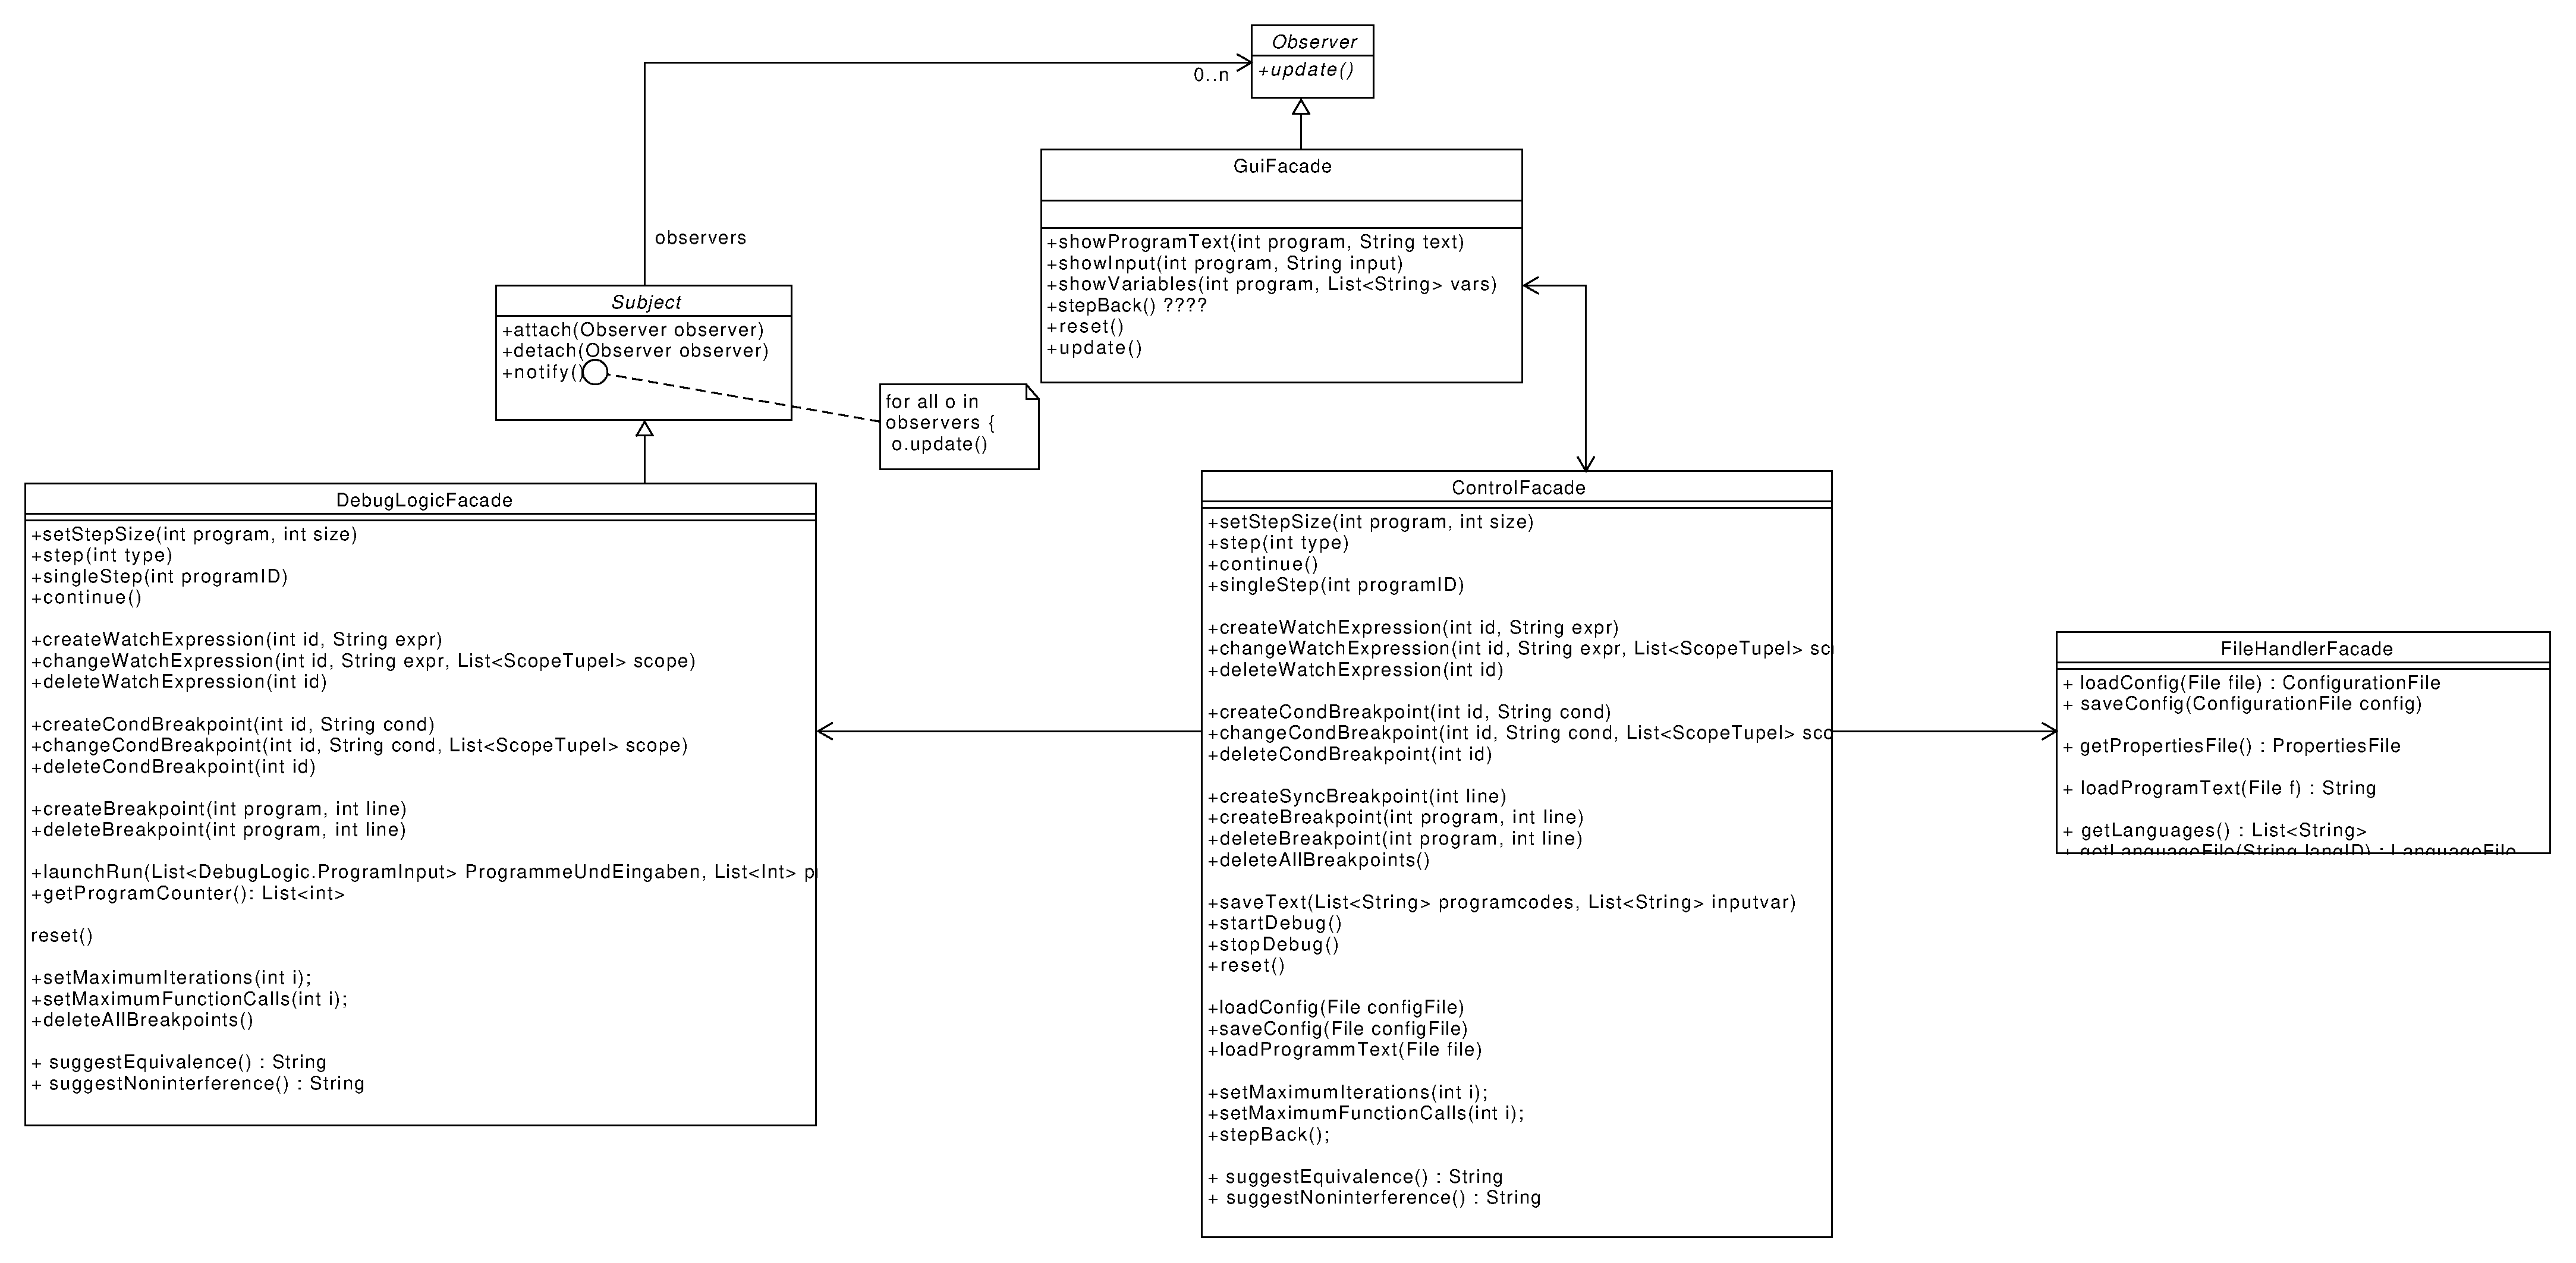
\includegraphics[width=1.42\textwidth]{diagrammIdeenUmlet/fassaden.pdf}}
\caption{Die Schnittstellen der Pakete durch Fassaden dargestellt}
\label{fig:fassaden}
\end{figure}
\paragraph{Das MVC-Pattern}
Im Entwurf wird das Architekturmuster Model-View-Controller (MVC) eingesetzt, um einen flexiblen Programmentwurf zu ermöglichen und die Erweiterbarkeit des Produkts sicher zu stellen. Die Pakete \textit{DebugLogic} und \textit{FileHandler} sind hierbei das Modell, welches die darzustellenden Daten enthält. Das \textit{UserInterface} ist die Präsentationsschicht, welche Benutzereingaben annimmt und die darzustellenden Werte über ein Beobachtermuster erhält. Die Steuerung, welche Benutzereingaben von der Präsentationsschicht erhält und diese auswertet, wird vom \textit{Control}-Paket bereitgestellt. \\
Alle Pakete stellen ihre Funktionalität über Fassadenklassen nach außen zur Verfügung (siehe Abbildung \ref{fig:fassaden}). Die genauen Schnittstellen sind also durch diese Klassen definiert.

\paragraph{Das Observerpattern im MVC}
Im Rahmen einer MVC-Architektur, ist es notwendig, dass die Viewkomponente eine Zustandsänderung des Modells sofort erfährt und darauf reagieren kann, indem sie sich die von ihr zur Anzeige benötigten Daten holt. Da es der Erweiterbarkeit wegen auch möglich sein soll, einmal mehrere verschiedene dieser beobachtenden Viewkomponenten ein Modell beobachten zu lassen, empfiehlt sich das Entwurfsmuster \enquote{Observer}. Die von diesem Pattern zur Verfügung gestellte 1-zu-n Abhängigkeit passt damit hervorragend zur vorliegenden Problemstellung: Aus Gründen der Wiederverwendbarkeit darf das Modell nicht festsetzen, welche und wie viele solcher Beobachter es hat. Die allgemein definierten Schnittstellen \textit{Observer} und \textit{Subject} ermöglichen dies. 
\paragraph{Das Fassadenpattern}
Durch die Einteilung des Systems in einzelne Subsysteme in Form von Paketen, ist es von Nöten, Schnittstellen dieser Subsysteme zu definieren. Diese sollten fest sein und sich bei Änderung der internen Struktur eines Subsystems nicht ändern, sodass das Geheimnisprinzip eingehalten wird. Um zusätzlich die Abhängigkeiten der Pakete zwischeneinander im Sinne einer losen Kopplung gering zu halten, bietet sich das Entwurfsmuster \enquote{Facade} an. Jegliche Kommunikation zwischen den in Abbildung \ref{fig:fassaden} beschriebenen Paketen findet also über Fassaden statt. Das ermöglicht, die Schnittstellen des Paketes an einer Stelle zu definieren, und festgelegte Eintrittspunkte für die Kommunikation zwischen den Paketen zu bieten.


\newpage
\section{Das Paket \enquote{User Interface}}
\label{UI}
%Hallo Joana, 
%so passt du das Kapitel am besten an (viel fehlt nicht mehr):
%brauchen wir noch mehr Klassendiagramme?
%Man sollte die verwendetetn Entwurfsmuster noch besser beschreiben (habs durch %Kommentare mal markiert), unsere bisherige Beschreibung kopiere ich dir mal ans %Ende des Kapitels
\subsection{Übersicht}
%Aufgaben, angebotene und genutze Schnittstellen , Benutztrealtion als Text
Das Paket \textit{UserInterface} stellt die Möglichkeit zur Kommunikation des Nutzers mit dem Produkt dar. Hierbei dient dieses Paket als View Teil des MVC-Konzepts. \\
Es wird eine Fassade angeboten, welche es ermöglicht, Variablen, Programmtexte und Eingaben anzuzeigen. Dieses Paket nutzt die Fassade des Paketes \textit{Control} und deren angebotene Schnittstellen, um an Informationen zu gelangen, die der Benutzer anfordert, und die Aktionen des Benutzers zur Ausführung weiterzugeben. \\
Für die Implementierung der Benutzeroberfläche wird die Bibliothek \textit{javax.swing} benutzt. Durch die Nutzung von Swing besteht der Grundaufbau des \textit{UserInterfaces} aus einem Kompositum.
\subsection{Wichtige Elemente des User Interface}
\begin{figure}[!h]
\centering
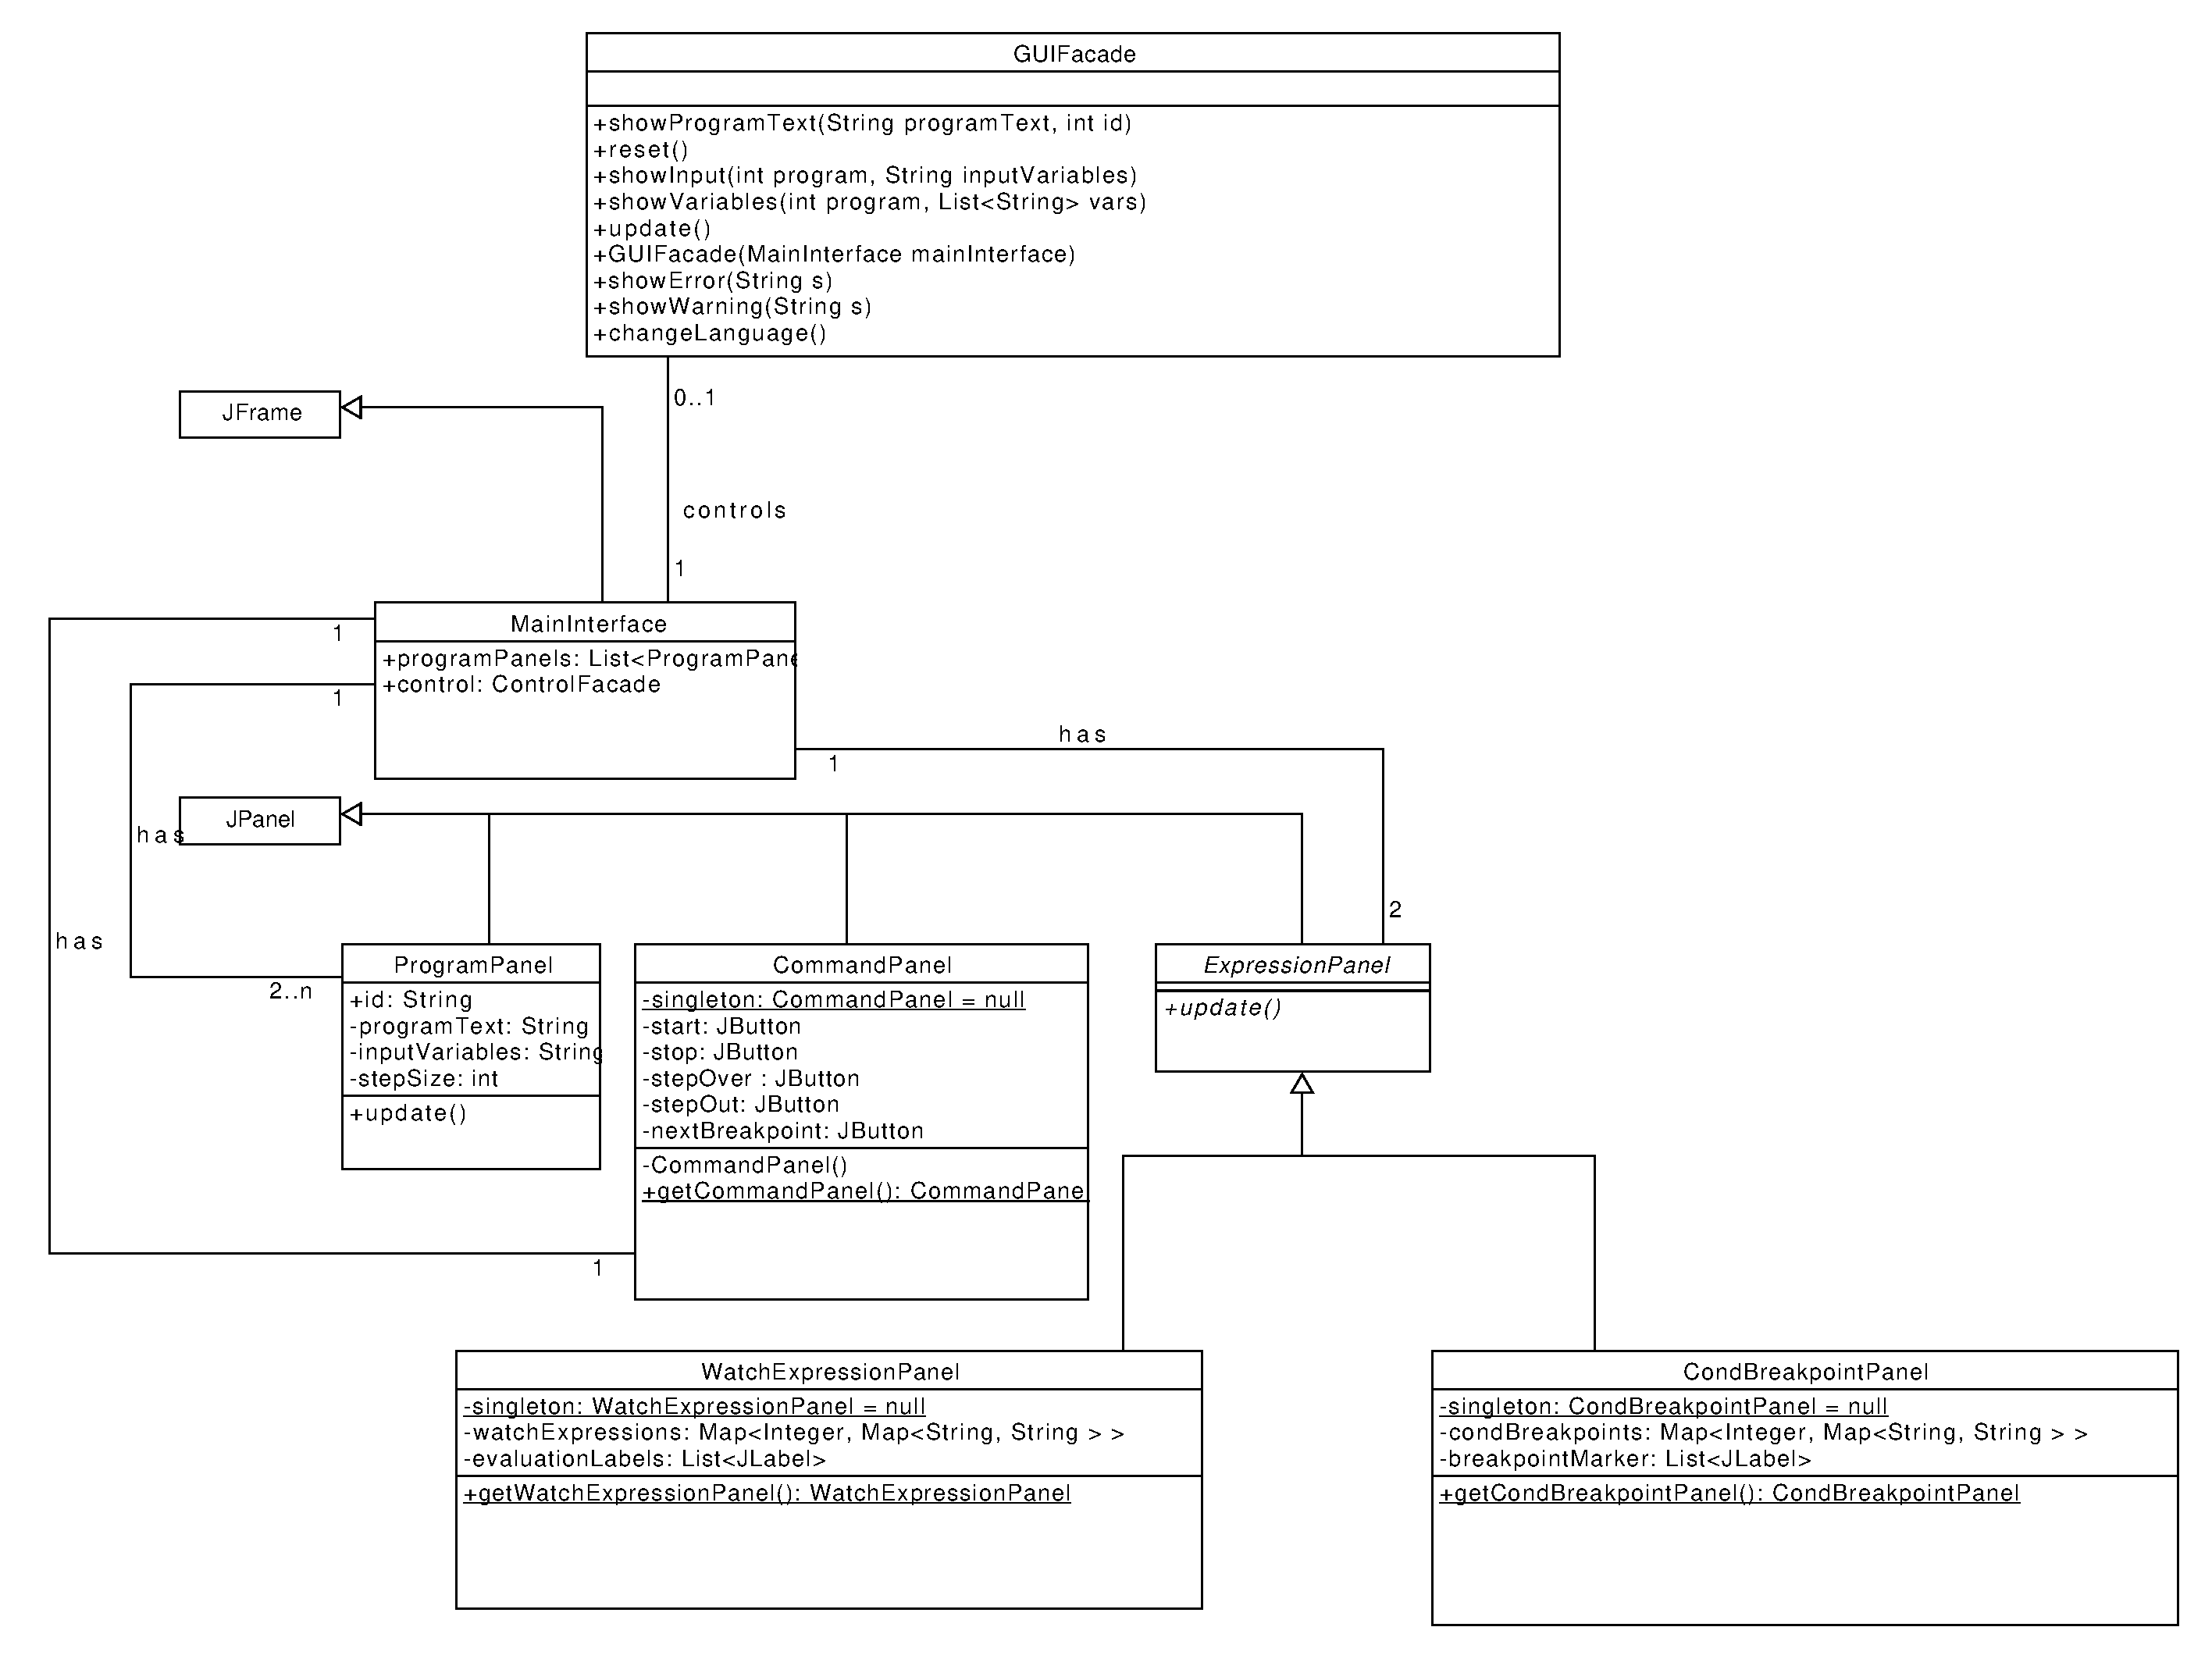
\includegraphics[width=1.1\textwidth]{diagrammIdeenUmlet/GUIOverview.pdf}
\caption{Wichtige Anzeigeelemente des User Interface}
\label{GUIOverview}
\end{figure}
\paragraph{GUIFacade}
Die Fassade der Benutzeroberfläche (\textit{GUIFacade}) dient zur Kommunikation mit den anderen Paketen. Um die Benutzeroberfläche einfach austauschen zu können, ist nur die Fassade mit den anderen Paketen verbunden, sodass alle anderen Klassen im Paket \textit{UserInterface} einfach ausgetauscht werden können. \\
Die Fassade bietet Methoden an, um Programmtexte und Eingabevariablen, sowie Fehlermeldungen oder Warnungen anzeigen zu können, und bietet die Möglichkeit, das User Interface zurückzusetzen. \\
Außerdem wird die \textit{GUIFacade} beim Start des Produkts im Rahmen des Beobachtermusters bei MVC (siehe Kapitel 3) bei der \textit{DebugLogic} als Beobachter angemeldet und besitzt eine \textit{update()}-Methode, über welche die Änderung der anzuzeigenden Daten gesteuert wird.
\paragraph{MainInterface}
 Das MainInterface bildet die Grundlage der Benutzeroberfläche. Diese Klasse enthält ein Liste an ProgramPanels , sowie ein CommandPanel und je ein WatchExpression bzw. CondBreakpointPanel. Sie ist verantwortlich für das Anzeigen von Menüs und diesen vier Panelarten, sowie für das Benachrichtigen des Benutzers mithilfe von DebuggerPopUps. 
\paragraph{ProgramPanel}
Ein ProgramPanel ist eine Anzeigeeinheit, die alle wichtigen Informationen zu einem einzelnen Programm anzeigt. Hierzu zählen der Programmtext, die Eingabevariablen, die Schrittgröße, der Programmname und die aktuelle Variablenbelegung. \\
Als Teil des Beobachter-Entwurfsmusters besitzt ein ProgramPanel eine update()-Methode, um bei Änderung der anzuzeigenden Daten benachrichtigt werden zu können.
\paragraph{CommandPanel}
Ein CommandPanel ist der Abschnitt, welcher die Buttons zur Kontrolle des Debugvorgangs anzeigt. Da ein solcher Kommandoblock nur ein mal benötigt wird, ist dieser als Singleton implementiert. 
\paragraph{ExpressionPanel}
Bei dieser Klasse handelt es sich um eine abstrakte Klasse, welche das Anzeigen von Ausdrücken ermöglicht. Für die Ausdrücke WatchExpression und CondBreakpoint wurden nicht abstrakte Unterklassen entworfen (WatchExpressionPanel und CondBreakpointPanel). Diese werden als Singletons realisiert, um einen globalen Zugriffspunkt auf die Instanzen zu erhalten, und um die alleinige Existenz eines Exemplars pro Klasse zu Sichern. \\
Als Teil des Beobachter-Entwurfsmusters besitzt ein ExpressionPanel eine update()-Methode, um bei Änderung der anzuzeigenden Daten benachrichtigt werden zu können.
\begin{figure}[!h]
\centering
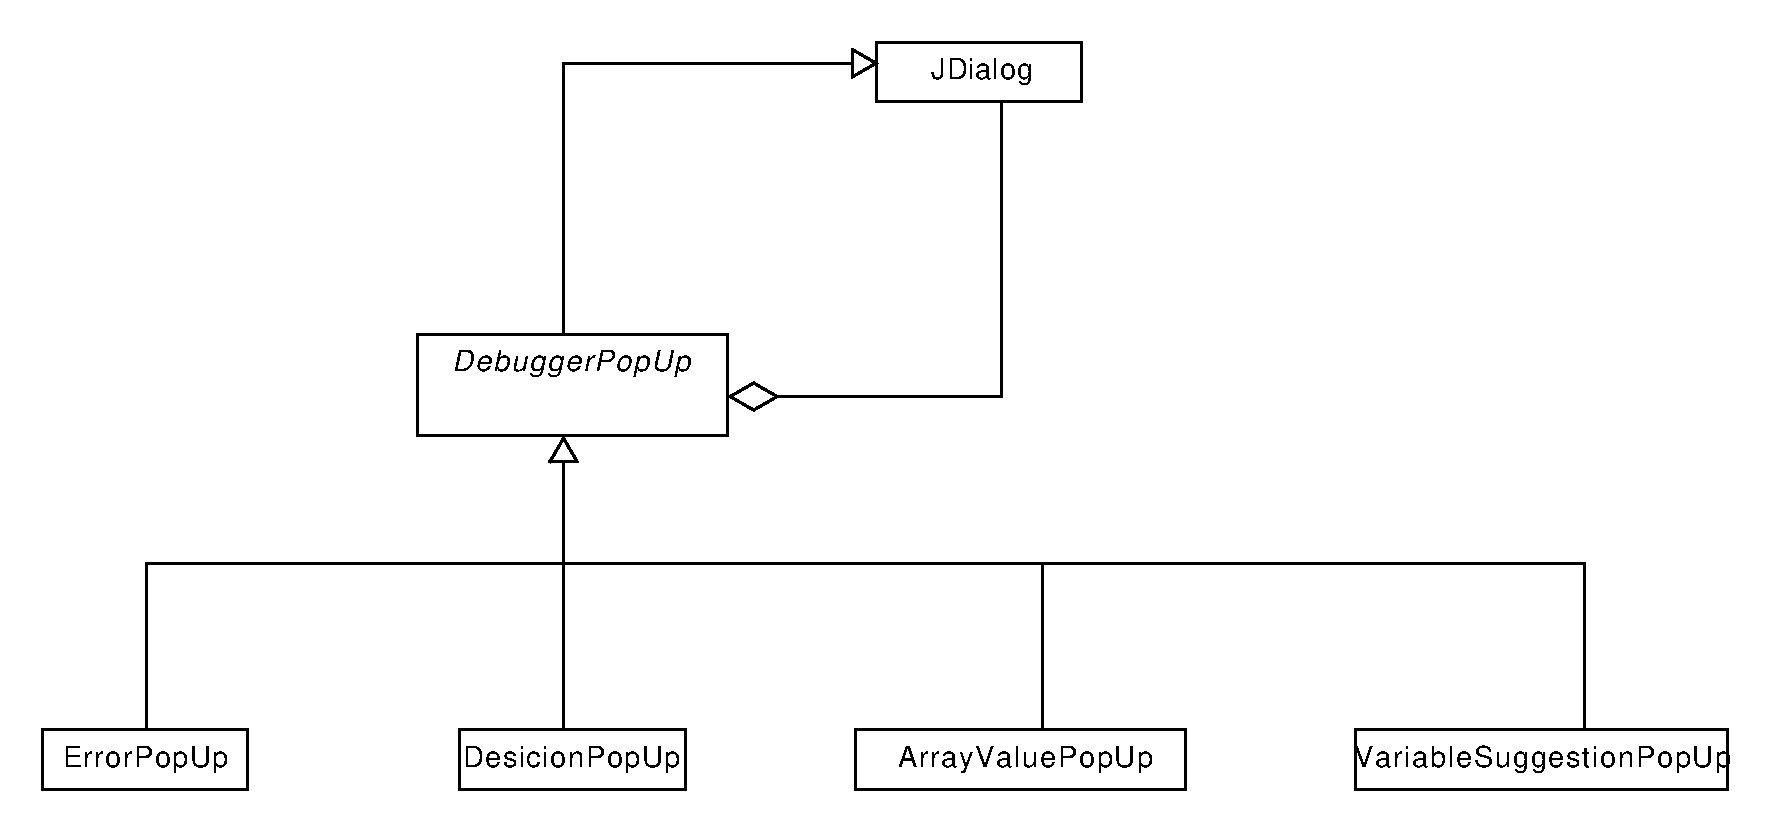
\includegraphics[width=0.8\textwidth]{diagrammIdeenUmlet/GUIDekorierer.pdf}
\caption{Realisierung des Entwurfsmusters Dekorierer in DebuggerPopUp}
\label{guidekorierer}
\end{figure}
\paragraph{DebuggerPopUp}
Ein DebuggerPopUp ist ein JDialog, welcher auf dieses Produkt ausgelegt ist. Es handelt sich um eine abstrakte Klasse, welche die nicht abstrakten Unterklassen ErrorPopUp, WarningPopUp, ArrayValuePopUp und VariableSuggestionPopUp hat. Diese Unterklassen, welche von DebuggerPopUp erben, sind darauf ausgelegt Fehlermeldungen, Warnungen oder Variablenwerte anzuzeigen. \\ 
Die Klasse DebuggerPopUp stellt, wie in Abbildung \ref{guidekorierer} zu Sehen, ein Dekorierer Entwurfsmuster mit JDialog dar.
%Warum Dekorierer?

\section{Das Paket \enquote{Control}}
\label{Control}
%Hallo Etienne, bitte pass ein Kapitel so an, damit es zu den anderen passt:
%Aus den Infos unter Übersicht einen schönen Fließtext machen, mit Hinblick auf %Gesamtfunktionalität.
%Ganze Sätze zur Beschreibung der wichtigen Klassen (siehe User Interface, im 
%Idealfall mit (kleinem) klassendiagramm und Erklärung, warum keine Patterns 
%benötigt werden
\subsection{Übersicht}
    Das Paket \textit{Control} entspricht dem Kontroll-Teil des Architekturstils MVC.\\
    Es dient der Entgegennahme von Benutzerinteraktionen auf dem \textit{UserInterface} und der Steuerung der Interaktion zwischen den Subsystemen \textit{UserInterface} und \textit{DebugLogic}.
    Schaltflächen, sowie Eingabefelder werden im Paket \textit{UserInterface} mit Präsentationskomponenten wie dem Variableninspektor zusammengefasst.\\
    Die vom Paket bereitgestellten Methoden sind über eine Fassade aufrufbar.\\
    \textit{Control} benutzt das Paket \textit{Debuglogic}, um Zustandsveränderungen des Datenmodells auszulösen.
    Beispielsweise kann das Modell aufgefordert werden, einen eingegebenen Quelltext oder spezifizierten Haltepunkt zu speichern oder zu löschen. 
    Weiter kann das Modell dazu aufgefordert werden, datenbezogene Aktionen auszuführen wie das Starten eines Debugvorgangs, oder das Durchführen eines Einzelschrittes. 
    Zum Ausführen von Speicher- und Ladeaufträgen benutzt \textit{Control} das Paket \textit{FileHandler}.
\subsection{Wichtige Elemente der Control}
    Um die Funktionalität des Paketes aufzuteilen, wurden vier Klassen entworfen, die jeweils unterschiedliche Zuständigkeit besitzen.
\paragraph{ControlFacade}
    \textit{ControlFacade} bietet eine Schnittstelle zum Paket \textit{Control}.

\begin{figure}[!h]
    \makebox[\textwidth][c]{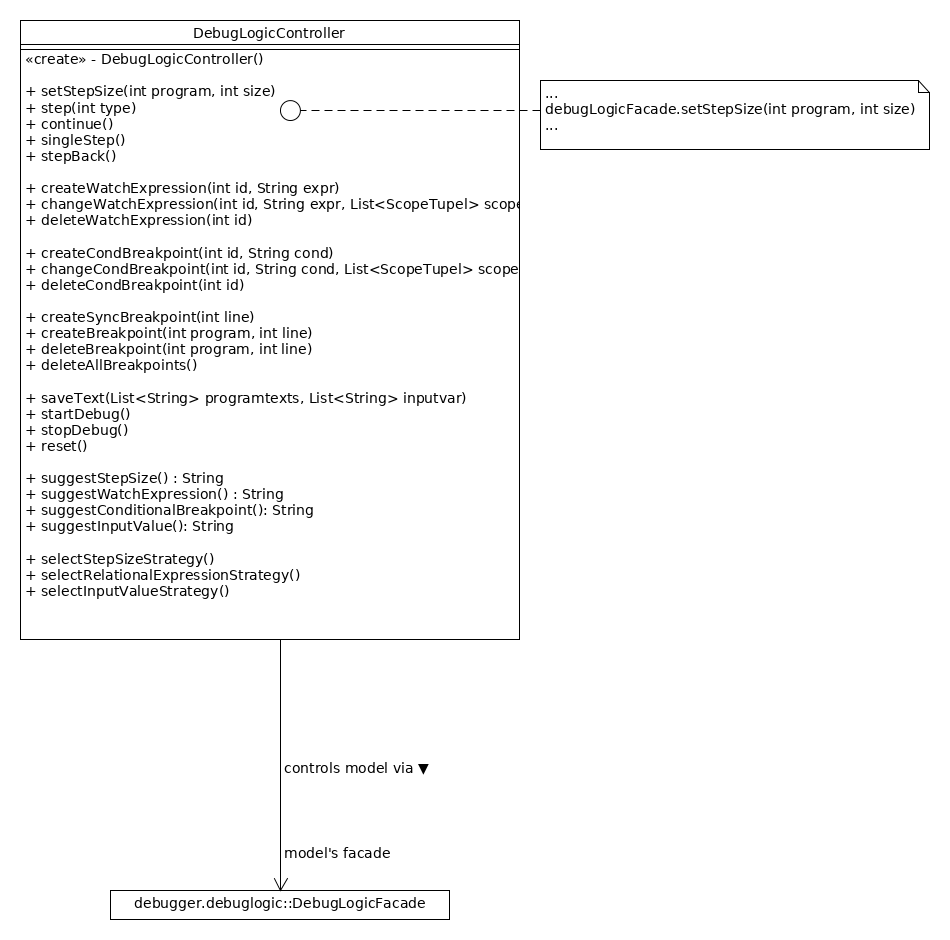
\includegraphics[width=0.8\textwidth]{diagrammIdeenUmlet/debuglogic_DebugLogicController.png}}
    \caption{Die Klasse DebugLogicController}
    \label{fig:DebugLogicController}
\end{figure}
\paragraph{DebugLogicController}
    \textit{DebugLogicController} ist für die Modifikation der Daten des Modells und das Aufrufen von Debugmechanismen zuständig.\\
    Über die bereitgestellten Methoden wird \enquote{DebugLogic} dazu aufgefordert, Schritte durchzuführen, WatchExpressions oder Haltepunkte zu erstellen und zu entfernen oder Vorschläge zu generieren.
    Außerdem werden die Zustände \enquote{Debugmodus} und \enquote{Editiermodus} in \textit{Control} implementiert, folglich bietet diese Klasse zwei Methoden zum Wechseln des aktuellen Modus.
\paragraph{ExceptionHandler}
    \textit{ExceptionHandler} dient zur Behandlung von beim Aufruf der Methoden aus DebugLogic oder FileHandler ausgelösten Ausnahmen.\\
    Insbesondere kann die Präsentation dazu aufgefordert werden, Benutzer der Anwendung entsprechend über eine Fehlersituation zu informieren.
\paragraph{FileHandlerInteractor}
    \textit{FileHandlerInteractor} ist verantwortlich für das Speichern und Laden von Konfigurationsdateien, sowie das Verwalten einer Sprachdatei, die Anzeigetexte für die Präsentation des \textit{UserInterface} enthält.\\
    Dementsprechend besitzt die Klasse Methoden, durch welche das Wiederherstellen gespeicherter Sitzungen, oder das Laden eines Programmtextes ermöglicht wird.
    Um dies zu ermöglichen, werden sowohl das Modell modifiziert, als auch die Präsentation (direkt) aufgefordert die gebotene Darstellung zu verändern.

\section{Das Paket \enquote{File Handler}}
\label{FileHandler}
% Hallo Pascal, 
%so passt du dein Kapitel am besten an, damit es zu den anderen passt:
%- Übersicht: alle Paragraphen, Aufzählungen rausmachen und einen schönen %Blocktext daraus machen.
%- Die Methoden hab ich schon rausgenommen, es ist allerdings immer noch echt  %viel. Manche sollten vielleicht genauer beschrieben werden, andere gar nicht. %Kann man ein paar davon als Gruppe gemeinsam beschreiben, mit Hinblick auf die %dadurch bereitgestellte Funktionalität? Vielleicht kannst du das mit den Readern %und Writern so lösen, wie die DebuggerPopUps oben? Dann kannnst du auch gleich %ein paar Ausschnitte aus dem Klassendiagramm einfügen und die benutzen Patterns %beschreiben. Deine bisherige Beschreibung der Patterns kopiere ich dir mal ganz %ans Ende.
\subsection{Übersicht}
%\paragraph{Aufgaben}
%Das Paket \textit{FileHandler} stellt die Funktionalität zum Lesen, Schreiben, %Parsen und Interpretieren von sämtlichen Dateien bereit und siedelt sich im %Model Teil des MVC-Konzepts an.
%Dabei wandelt der \textit{FileHandler} eine Konfigurationsdatei, welche auf dem Dateisystem gespeichert ist, in eine virtuelle Datei um.
%Diese besteht aus einer Klassenstruktur, welche äquivalent zur Definition des Speicherformats ist, also aus Zuweisungen und Blöcken.
%Weiter erzeugt der FileHandler Objekte der Konfigurations-, Sprach- und Einstellungsdateien und kann diese nach außen weitergeben.
%\paragraph{Schnittstellen}
%\begin{itemize}
%\item Genutzte Schnittstellen: \\
%Der FileHandler benötigt keine Schnittstellen anderer Programmpakete, da er an unterster Stelle in der Benutztrelation steht.
%\item Angebotene Schnittstellen: \\
%Es werden eine Fassade und drei Klassen angeboten.
%Diese repräsentieren die Dateien für Produkteinstellungen, Sprachen (Übersetzungen der GUI) und Laufkonfigurationen.
%\end{itemize}
%\paragraph{Benutztrelation}
%Der FileHandler benutzt keine weiteren Subsysteme.
Das Paket \textit{FileHandler} stellt die Funktionalität zum Lesen, Schreiben, Parsen und Interpretieren von sämtlichen Dateien bereit und siedelt sich im Model Teil des MVC-Konzepts an.
Dabei wandelt der \textit{FileHandler} eine Konfigurations- oder Sprachdatei, welche auf dem Dateisystem gespeichert ist, in eine virtuelle Datei um.
Diese besteht aus einer Klassenstruktur, welche äquivalent zur Definition des Speicherformats (siehe Anhang \ref{Anhang}) ist, also aus Zuweisungen und Blöcken.
Weiter erzeugt der \textit{FileHandler} Objekte der Konfigurations-, Sprach- und Einstellungsdateien und kann diese nach außen weitergeben.
Einstellungsdateien werden mithilfe von Java's Properties Klasse realisiert.
Da der FileHandler an unterster Stelle der Benutztrelation steht, benötigt er keine Schnittstellen anderer Programmpakete, lediglich werden mindestens jeweils eine Klasse zum Lesen und Schreiben von Konfigurations-, Einstellungs- und Sprachdateien benötigt.
Dafür werden Klassen für das interne Relational Debugger Format (RDBF)  beziehungsweise Java Properties bereitgestellt. Jedoch kann das Paket um andere Formate, wie \enquote{XML} oder \enquote{Json}, erweitert werden.
Weiter werden eine Fassadenklasse und drei Klassen für das Speichern von Produkteinstellungen, Sprachen (Übersetzungen der GUI) und Konfigurationen angeboten und nach außen weitergegeben.
\subsection{Wichtige Elemente des File Handlers}
\subsubsection{Unterpaket FileHandler.Facade}
\begin{figure}[!h]
\makebox[\textwidth][c]{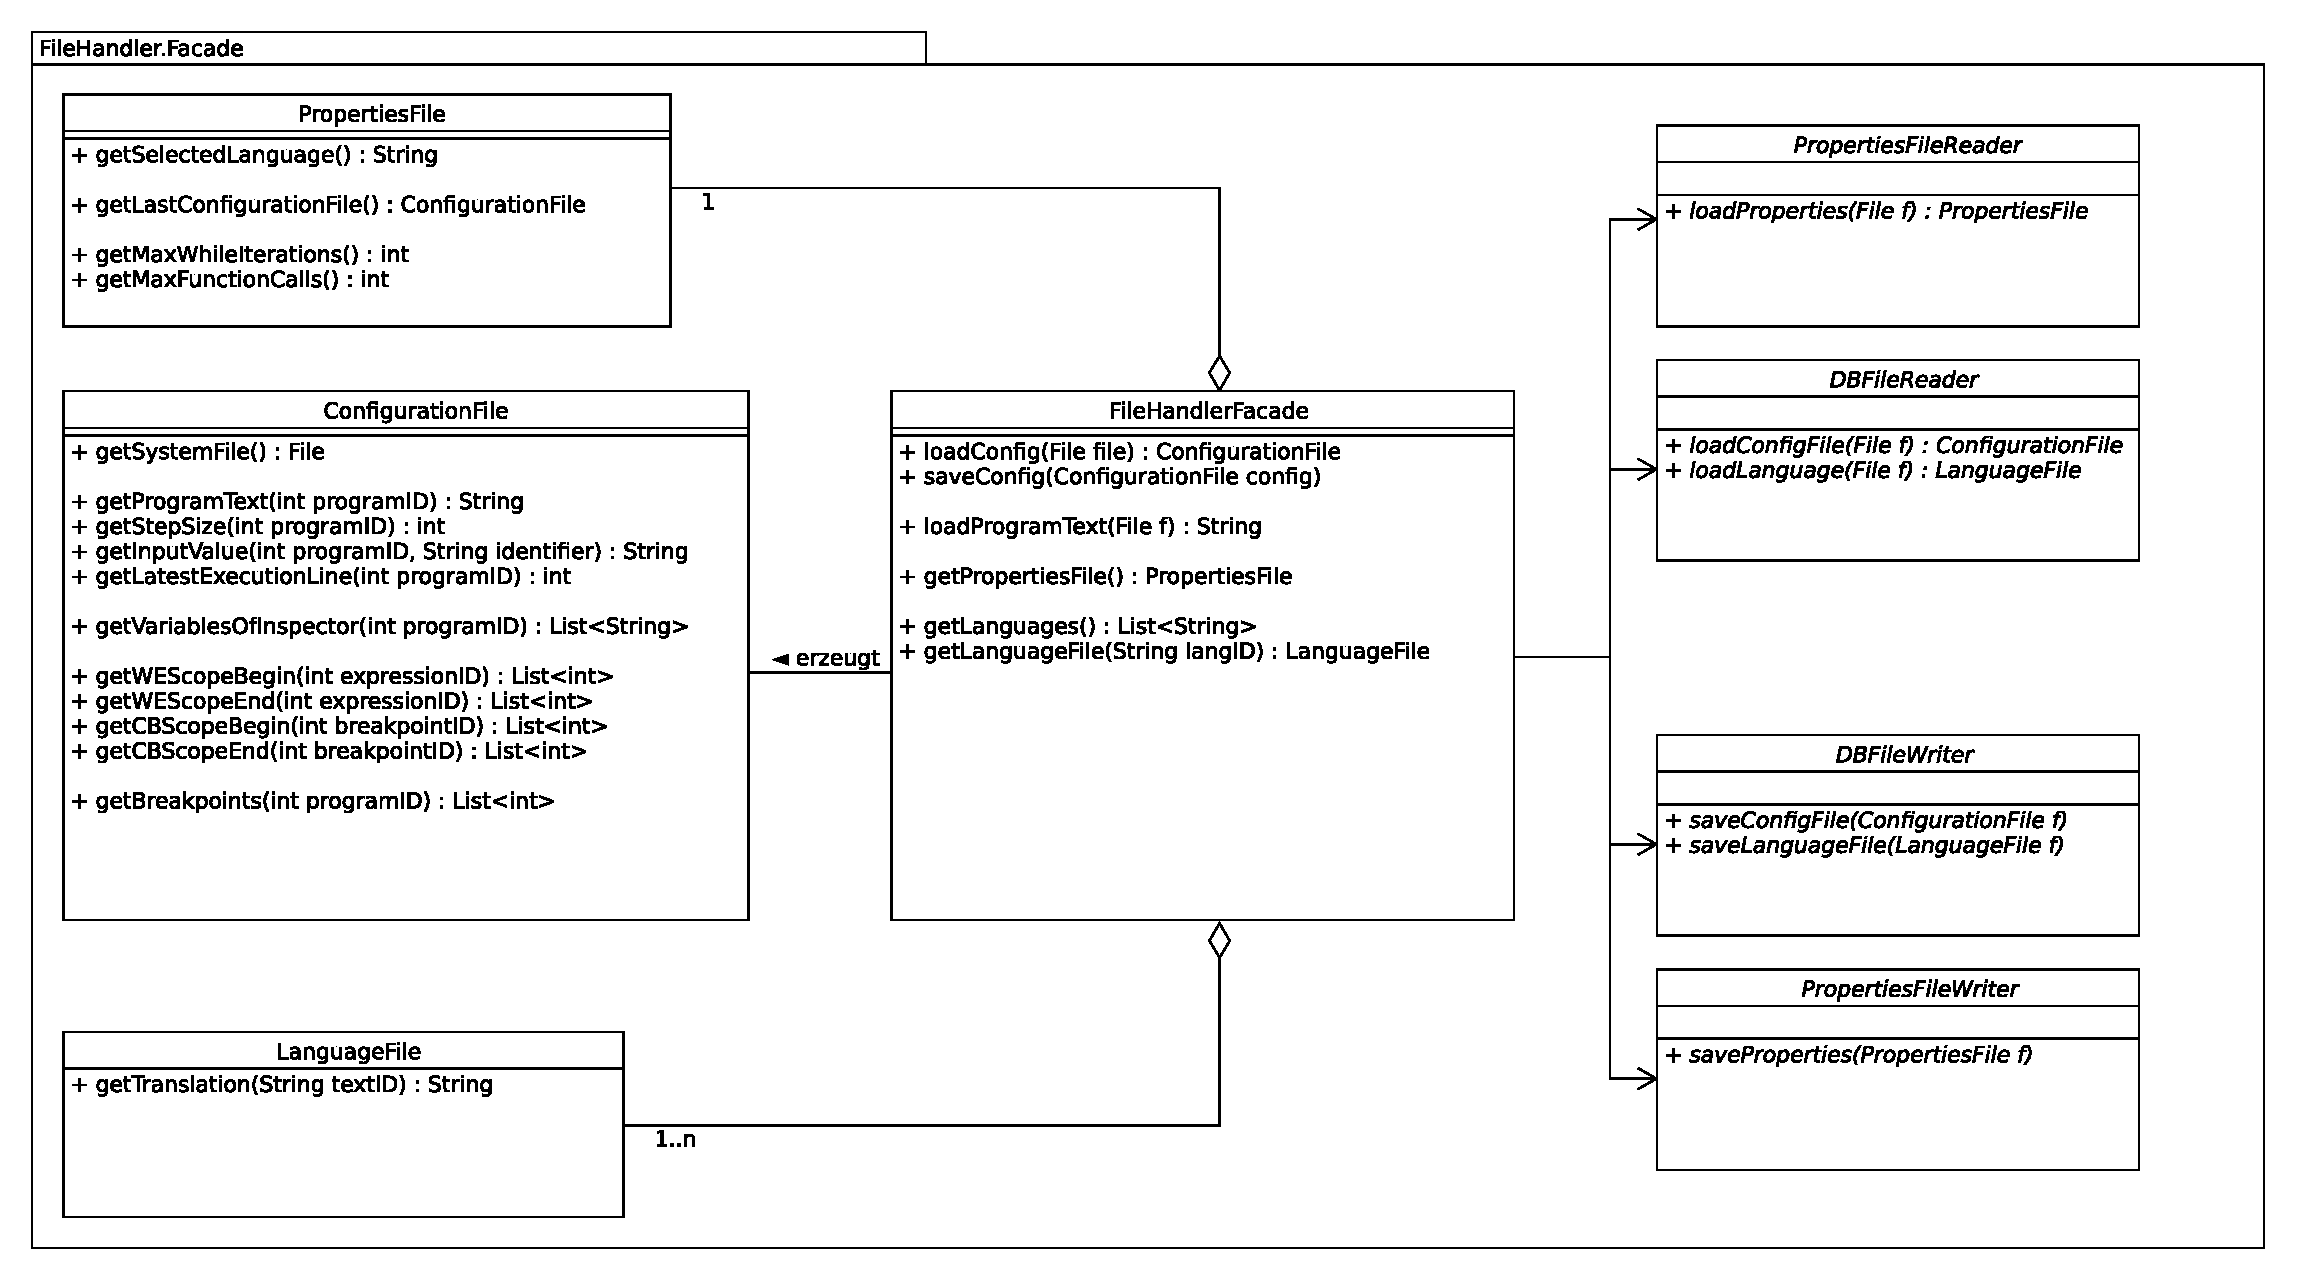
\includegraphics[width=0.95\textwidth]{diagrammIdeenUmlet/Filehandler_Ansicht1.pdf}}
\caption{Die Schnittstellen Fassade des File Handlers}
\label{fig:facade_fileHandler}
\end{figure}
\paragraph{FileHandlerFacade}
Diese Klasse speichert alle verfügbaren Sprachen und hilft bei der Erzeugung von Konfigurations- und Einstellungsdateien.
%bietet wofür Methoden an?
Die Klasse beinhaltet alle aktuellen Sprachdateien.
Sie bietet Methoden zum Lesen und Speichern von Konfigurationsdateien an. Dabei können auch Textdateien, die einen Programmtext enthalten gelesen werden.
Weiter kann die aktuelle Einstellungsdatei abgerufen werden, sowie alle verfügbaren Sprachen und eine bestimmte Sprachdatei.
\paragraph{ConfigurationFile}
Diese Klasse speichert eine Konfiguration des Debuggers.
%bietet wofür Methoden an?
Dabei enthält diese Objekte für den Speicherort der Konfiguration, sowie Programmtexte, Schrittgrößen und Eingabewerte.
Weiter wird der Status des Debuggers gespeichert, also die derzeitigen Programmzähler, Watch-Expressions, Breakpoints (einfach und bedingt), sowie der von die von der GUI abhängigen Konfiguration der Variableninspektors.
Methoden zum Lesen und Schreiben dieser Attribute werden zur Verfügung gestellt. Dabei wird darauf geachtet, dass nicht zuviel von der internen Struktur der Klasse nach außen gegeben wird.
\paragraph{PropertiesFile}
Diese Klasse speichert die Einstellungen des Debuggers.
%Beispiele / bietet wofür Methoden an?
Darunter fallen Daten wie die ausgewählte Sprache, obere Grenzen für Iterationen und die zuletzt verwendete Konfigurationsdatei, falls diese existiert.
Methoden für diese Attribute werden durch einfache Getter realisiert.
\paragraph{LanguageFile}
%ganzer Satz, bietet wofür Methoden an?
Diese Klasse stellt die Übersetzung in eine bestimmte Sprache zu den von einem User Interface angezeigten Texten bereit.
Hierbei zählen nicht nur Anzeigeelemente, sondern auch geworfene Fehlermeldungen der unteren Schichten.
Somit wird eine Methode zum transformieren einer Identität in einen Text bereitgestellt.

%TODO Irgendwie eine Referenz der Strategie auf die nächsten 4 Klassen machen
%\paragraph{DBFileReader}
%Der DIbugger(DB) FileReader dient als Schnittstelle von der FileHandlerFacade zum Dateisystem für das Lesen von verschiedenen Dateiformaten für Konfigurations- und Sprachdateien.
%bietet wofür Methoden an?
%Es werden hier nur abstrakte Methoden zum Lesen der oben genannten Dateien bereitgestellt.
%\paragraph{PropertiesFileReader}
%Als abstrakte Klasse dient \textit{PropertiesFileReader} als Schnittstelle zum Lesen einer Einstellungsdatei und bietet hierbei nur eine abstrakte Methode zum Lesen dieser an.
%ganzer Satz, bietet wofür Methoden an?
%\paragraph{DBFileWriter}
%Diese Klasse dient als Schnittstelle von der \textit{FileHandlerFacade} zum Dateisystem für das Schreiben in verschiedene Dateiformate von Konfigurations- und Sprachdateien.
%ganzer satz, bietet wofür Methoden an?
%Auch hier werden nur abstrakte Methoden angeboten, welche für das Schreiben von oben genannten Dateien genutzt werden können.
%\paragraph{PropertiesFileWriter}
%Der \textit{PropertiesFileWriter} dient als Schnittstelle zum Schreiben einer Einstellungsdatei.
%du weißt schon... ja ganzer satzt und methoden
%Es wird eine abstrakte Methode angeboten, welche für das Schreiben einer Einstellungsdatei benutzt werden kann.

\paragraph{FileReader / Writer Klassen}
Zum Lesen und Schreiben der Konfigurations-, Einstellungs- und Sprachdateien werden vier abstrakte Klassen \textit{DB(DIbugger)FileReader},\textit{PropertiesFileReader},\textit{DBFileWriter} und \textit{PropertiesFileWriter}
angeboten. Diese stehen jeweils für die Basis einer Strategie und bieten zusammen abstrakte Methoden zum Lesen und Schreiben der oben genannten Dateien an.

\subsubsection{Unterpaket FileHandler.RDBF}
\begin{figure}[!h]
\makebox[\textwidth][c]{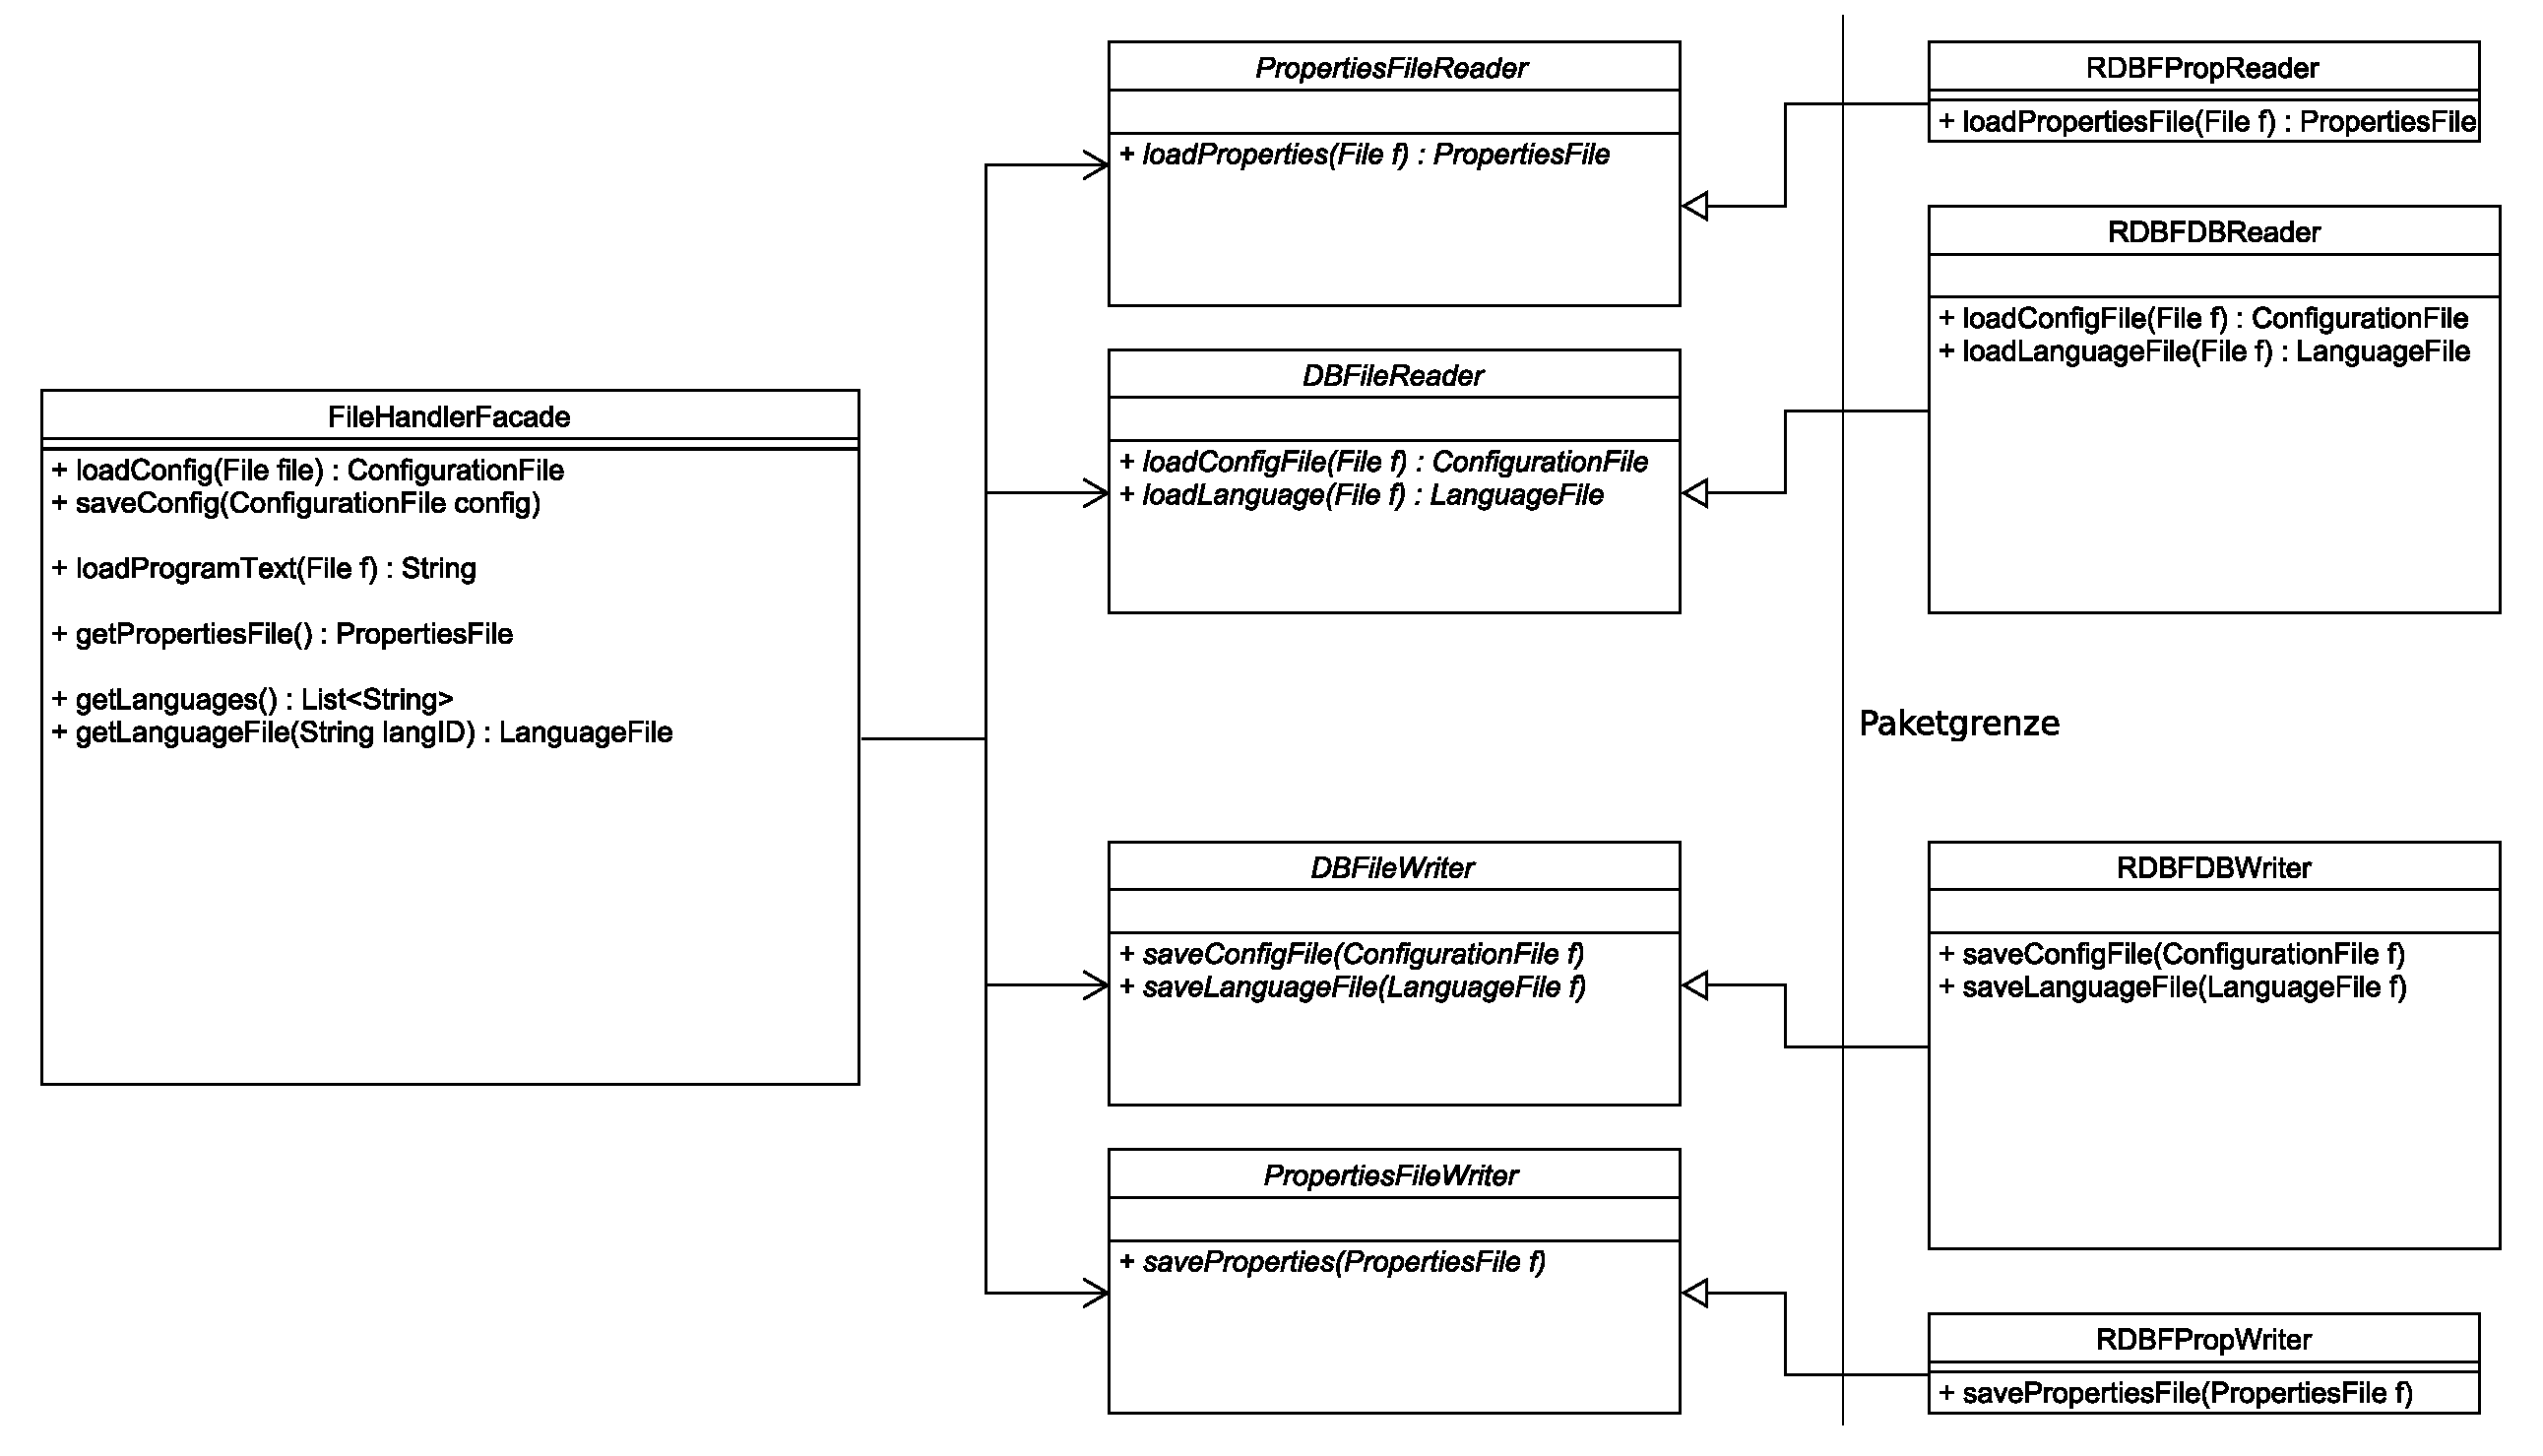
\includegraphics[width=1.0\textwidth]{diagrammIdeenUmlet/Filehandler_Ansicht2.pdf}}
\caption{Das Strategie Entwurfsmuster im FileHandler}
\label{fig:debuggerOverview}
\end{figure}

Dieses Paket bietet als untergeordnete konkrete Strategie für das Lesen und Schreiben der Konfigurations-, Einstellungs, und Sprachdateien formatiert im Relational Debugger Format (RDBF) Klassenstrukturen und Methoden an.
Das Speicherformat RDBF kann im Anhang \ref{RDBF} eingesehen werden.
%--------------------------TODO---------------------------------%
%\paragraph{RDBFDBReader}
%Diese Klasse stellt Funktionalität zum Lesen von Sprach- und Konfigurationsdateien im RDBF Format bereit.
%%gilt ab sofort für alles was noch kommt.. scheiße ist das viel... da hast du recht
%Als konkrete Strategie werden die Methoden von der Klasse DBReader überschrieben.
%\paragraph{RDBFPropReader}
%Der \textit{RDBFPropReader} stellt Funktionalität zum Lesen der Einstellungsdatei bereit.
%\paragraph{RDBFDBWriter}
%Der \textit{RDBFDBWriter} stellt Funktionalität zum Schreiben von Sprach- und Konfigurationsdateien im RDBF Format bereit.
%\paragraph{RDBFPropWriter}
%Diese Klasse stellt Funktionalität zum Speichern der Einstellungsdatei bereit.

\paragraph{Konkrete Strategien zu den oben gennanten FileReader / Writer Klassen}
Als konkerete Implementierungen der DBFileReader, -Writer und PropertiesFileReader, -Writer Klassen werden vier Unterklassen angeboten.
Nennenswert tragen sie den selben Klassennamen wie obige, jedoch mit Präfix RDBF.
Die Klassen stellen jeweils eine Implementierung zum Lesen und Schreiben von Konfigurations- und Sprachdateien im RDBF Format, sowie Einstellungsdateien im Java Properties Format zur Verfügung.
Dabei stellen sie eine konkrete Strategie dar, um somit Austauschbar und Erweiterbar für weitere Strategien wie XML und Json zu sein.

\paragraph{RDBFReader}
Diese Klasse stellt Funktionalität zum Lesen von Dateien im RDBF Format bereit.
Dabei wird eine Methode zum Einlesen einer RDBF Datei bereitgestellt, die ein RDBFFile zurückgibt.
\paragraph{RDBFWriter}
Diese Klasse stellt Funktionalität zum Speichern von RDBFFile Objekten im RDBF Format bereit.
Es wird nur eine Methode angeboten, welche eine virtuelle RDBF Datei auf das Dateisystem des Nutzers schreibt.
%---------------------------------------------------------------%
\paragraph{RDBFParser}
Diese Klasse existiert als Singleton und übernimmt die Funktionalität, eingelesene Zeilen zu analysieren und zu interpretieren, um diese dann final zu Objekten zusammenzufassen.
Sie bietet Methoden zum herausfinden des Typs einer Zeile (Zuweisung, Block, Textblock), sowie eines Zuweisungswertes an.
Damit können weitere Methoden benutzt werden, welche aus einer Zuweisung die Variable und den Wert herausfinden, bei einem Block den Blocknamen und den Wert einer Zuweisung in einen primitiven Datentyp von JAVA umwandelt.
\paragraph{RDBFAdditions}
Abstrakte Klasse zum repräsentieren von RDBFFile und RDBFBlock, da diese sich nur in wenigen Punkten unterscheiden.
Hierfür werden eine Liste an Blöcken (RDBFBlock) und Daten (RDBFData) gespeichert und Getter-Methoden bereitgestellt.
Diese können mithilfe von Blocknamen und Variablennamen Teillisten der obigen Attribute erstellen und zurückgeben.
\paragraph{RDBFFile}
Repräsentiert eine RDBF Datei als schnell zugreifbare Objektstruktur und stützt sich dabei auf die Implementierung von RDBFAdditions.
Sie speichert zusätzlich nur den Dateipfad der darzustellenden Datei.
\paragraph{RDBFBlock}
Stellt einen in der RDBF Grammatik definierten Block dar. Dabei werden die Methoden von RDBFAdditions geerbt.
Die Klasse speichert zusätzlich zu beiden Listen nur den Namen des Blocks.
\paragraph{RDBFData}
Repräsentiert eine Zuweisung der RDBF Grammatik als Datenstruktur. Hierbei enthält diese einen Variablennamen, Wert und zusätzlich den Typ des Wertes.
Einfache Getter und Setter Methoden für die Attribute existieren.
\subsubsection{Unterpaket FileHandler.Exceptions}
\paragraph{Interface: FileHandlerException}
Dieses Interface sorgt dafür, dass alle Klassen im Unterpaket Exceptions des FileHandlers die benötigten Methoden für eine \textit{FileHanderException} haben.
\\
Alle Klassen in diesem Unterpaket implementieren die Schnittstelle \textit{FileHandlerException}.
%\paragraph{LanguageNotFoundException}
%Ausnahme, die ausgelöst wird, falls eine Sprachdatei nicht gefunden wurde.
%\paragraph{ParseBlockException}
%Ausnahme, die ausgelöst wird, falls beim Versuch, einen Datenblock zu parsen, ein Feler entsteht.
%\paragraph{ParseAssignmentException}
%Ausnahme, die ausgelöst wird, falls beim Versuch, eine Zuweisung zu parsen, kein zulässiger Datentyp existiert oder die Syntax fehlerhaft ist.
%\paragraph{InvalidLineTypeException}
%Ausnahme, die ausgelöst wird, falls der Typ einer Zeile nicht existent ist, also kein DatenBlock, TextBlock oder Zuweisung ist.
%\subsection{Patterns im Paket File Handler}
%Das Paket FileHandler.Facade stellt vier abstrakte Klassen zum Lesen und Schreiben von Sprach-, Einstellungs- und Konfigurationsdateien bereit. Dadurch wird das \enquote{Strategie}-Muster implementiert und vom Paket FileHandler.RDBF genutzt. Dabei wird für jede Abstrakte Klasse eine spezielle Strategie zur Verfügung gestellt. Jedoch können später weitere zum Lesen und Schreiben von anderer Dateiformaten, z.B. XML, Json... , implementiert werden. Somit dient die Verwendung des Musters vor allem der Erweiterbarkeit.\\
%Das Entwurfsmuster Einzelstück (Singleton) wurde bei der Klasse RDBFParser verwendet, da diese keine Daten speichern muss und nur für das Lesen und richtige Interpretieren von Zeilen verantwortlich ist. So wird  ein globaler Zugriffspunkt bereitgestellt und es wird sichergestellt, dass stets nur ein Parser exisitiert.
Es existieren die Klassen LanguageNotFounrException, ParseBlockException, ParseAssignmentException und InvalidLineTypeException.
Die LanguageNotFoundException tritt auf, falls eine nicht existente Sprache angefragt wird.
Alle anderern Exceptions behandeln das Auftreten von Fehlern während dem Auslesen von einzelnen Zeilen.
Dabei werden Methodenaufrufe auf falsche Zeilen, sowie syntaktisch falsche zeilen berügsichtigt.
\newpage
\section{Das Paket \enquote{Debug Logic}}
\label{DebugLogic}
%Hallo Bene,
%so passt du das Kapitel am Besten an, dass es zu den anderen passt:
%Aus Aufgaben / Schnittstellen / Benutztrelation jeweils zur Übersicht einen %schönen Blocktext machen, Inhalt ist ja schon da.
%Bei der Beschreibung der wichtigen Elemente an der Beschreibung im User %Interface orientieren, am besten gleich an der jeweiligen Stelle auf die %Patterns verweisen
%Die bisherige Beschreibung der Patterns habe ich dir ans Ende des Kapitels %kopiert.
Das Paket \textit{DebugLogic} stellt den Model Teil der MVC Architektur dar. Die interne Struktur des Paketes ist eine intransparente 3-Schichten-Architektur.\\
Die unterste Schicht stellt das Subpaket \textit{DebugLogic.AntlrParser} dar. Es erzeugt aus einfachen Zeichenketten Ableitungsbäume nach den Ableitungsregeln der im Anhang \ref{Anhang} gegebenen Grammatiken.\\ Darauf aufbauend in der mittleren Schicht findet sich das Subpaket \textit{DebugLogic.Interpreter}, das die Aufgabe hat, diese Ableitungsbäume durch Interpretieren in eine abstrakte und leicht handhabbare Form zu bringen. In der obersten Schicht ist das Subpaket \textit{DebugLogic.Debugger} angesiedelt. Dieses nutzt die abstrakten Repräsentationen und führt den eigentlichen Debugprozess darauf aus.
\subsection{Debugger}
\subsubsection{Übersicht}
Der Debugger nutzt die vom Subpaket \textit{DebugLogic.Interpreter} erzeugten Informationen, um Watch-Expressions und bedingte Breakpoints auszuwerten, sowie die üblichen Debugmechanismen zu steuern.
%\subparagraph{Schnittstellen}
Als oberste Schicht des Paketes \textit{DebugLogic} stellt dieses Subpaket die gleichen Schnittstellen wie die DebugLogic bereit. Diese können in Kapitel \ref{GlobalePatterns} der entsprechenden Fassadenklasse entnommen werden. \\
%\subparagraph{Benutztrelation} 
Um die üblichen Debugmechanismen wie Schritte und Weiter durchführen zu können, nutzt dieses Subpaket den vom Subpaket \textit{DebugLogic.Interpreter} bereitgestellten Trace-Iterator. 
Um WatchExpressions und bedingte Breakpoints auszuwerten und zu repräsentieren, nutzt dieses Subpaket die vom Subpaket \textit{DebugLogic.Interpreter} bereitgestellte abstrakte Repräsentationen.
\begin{figure}[!h]
\makebox[\textwidth][c]{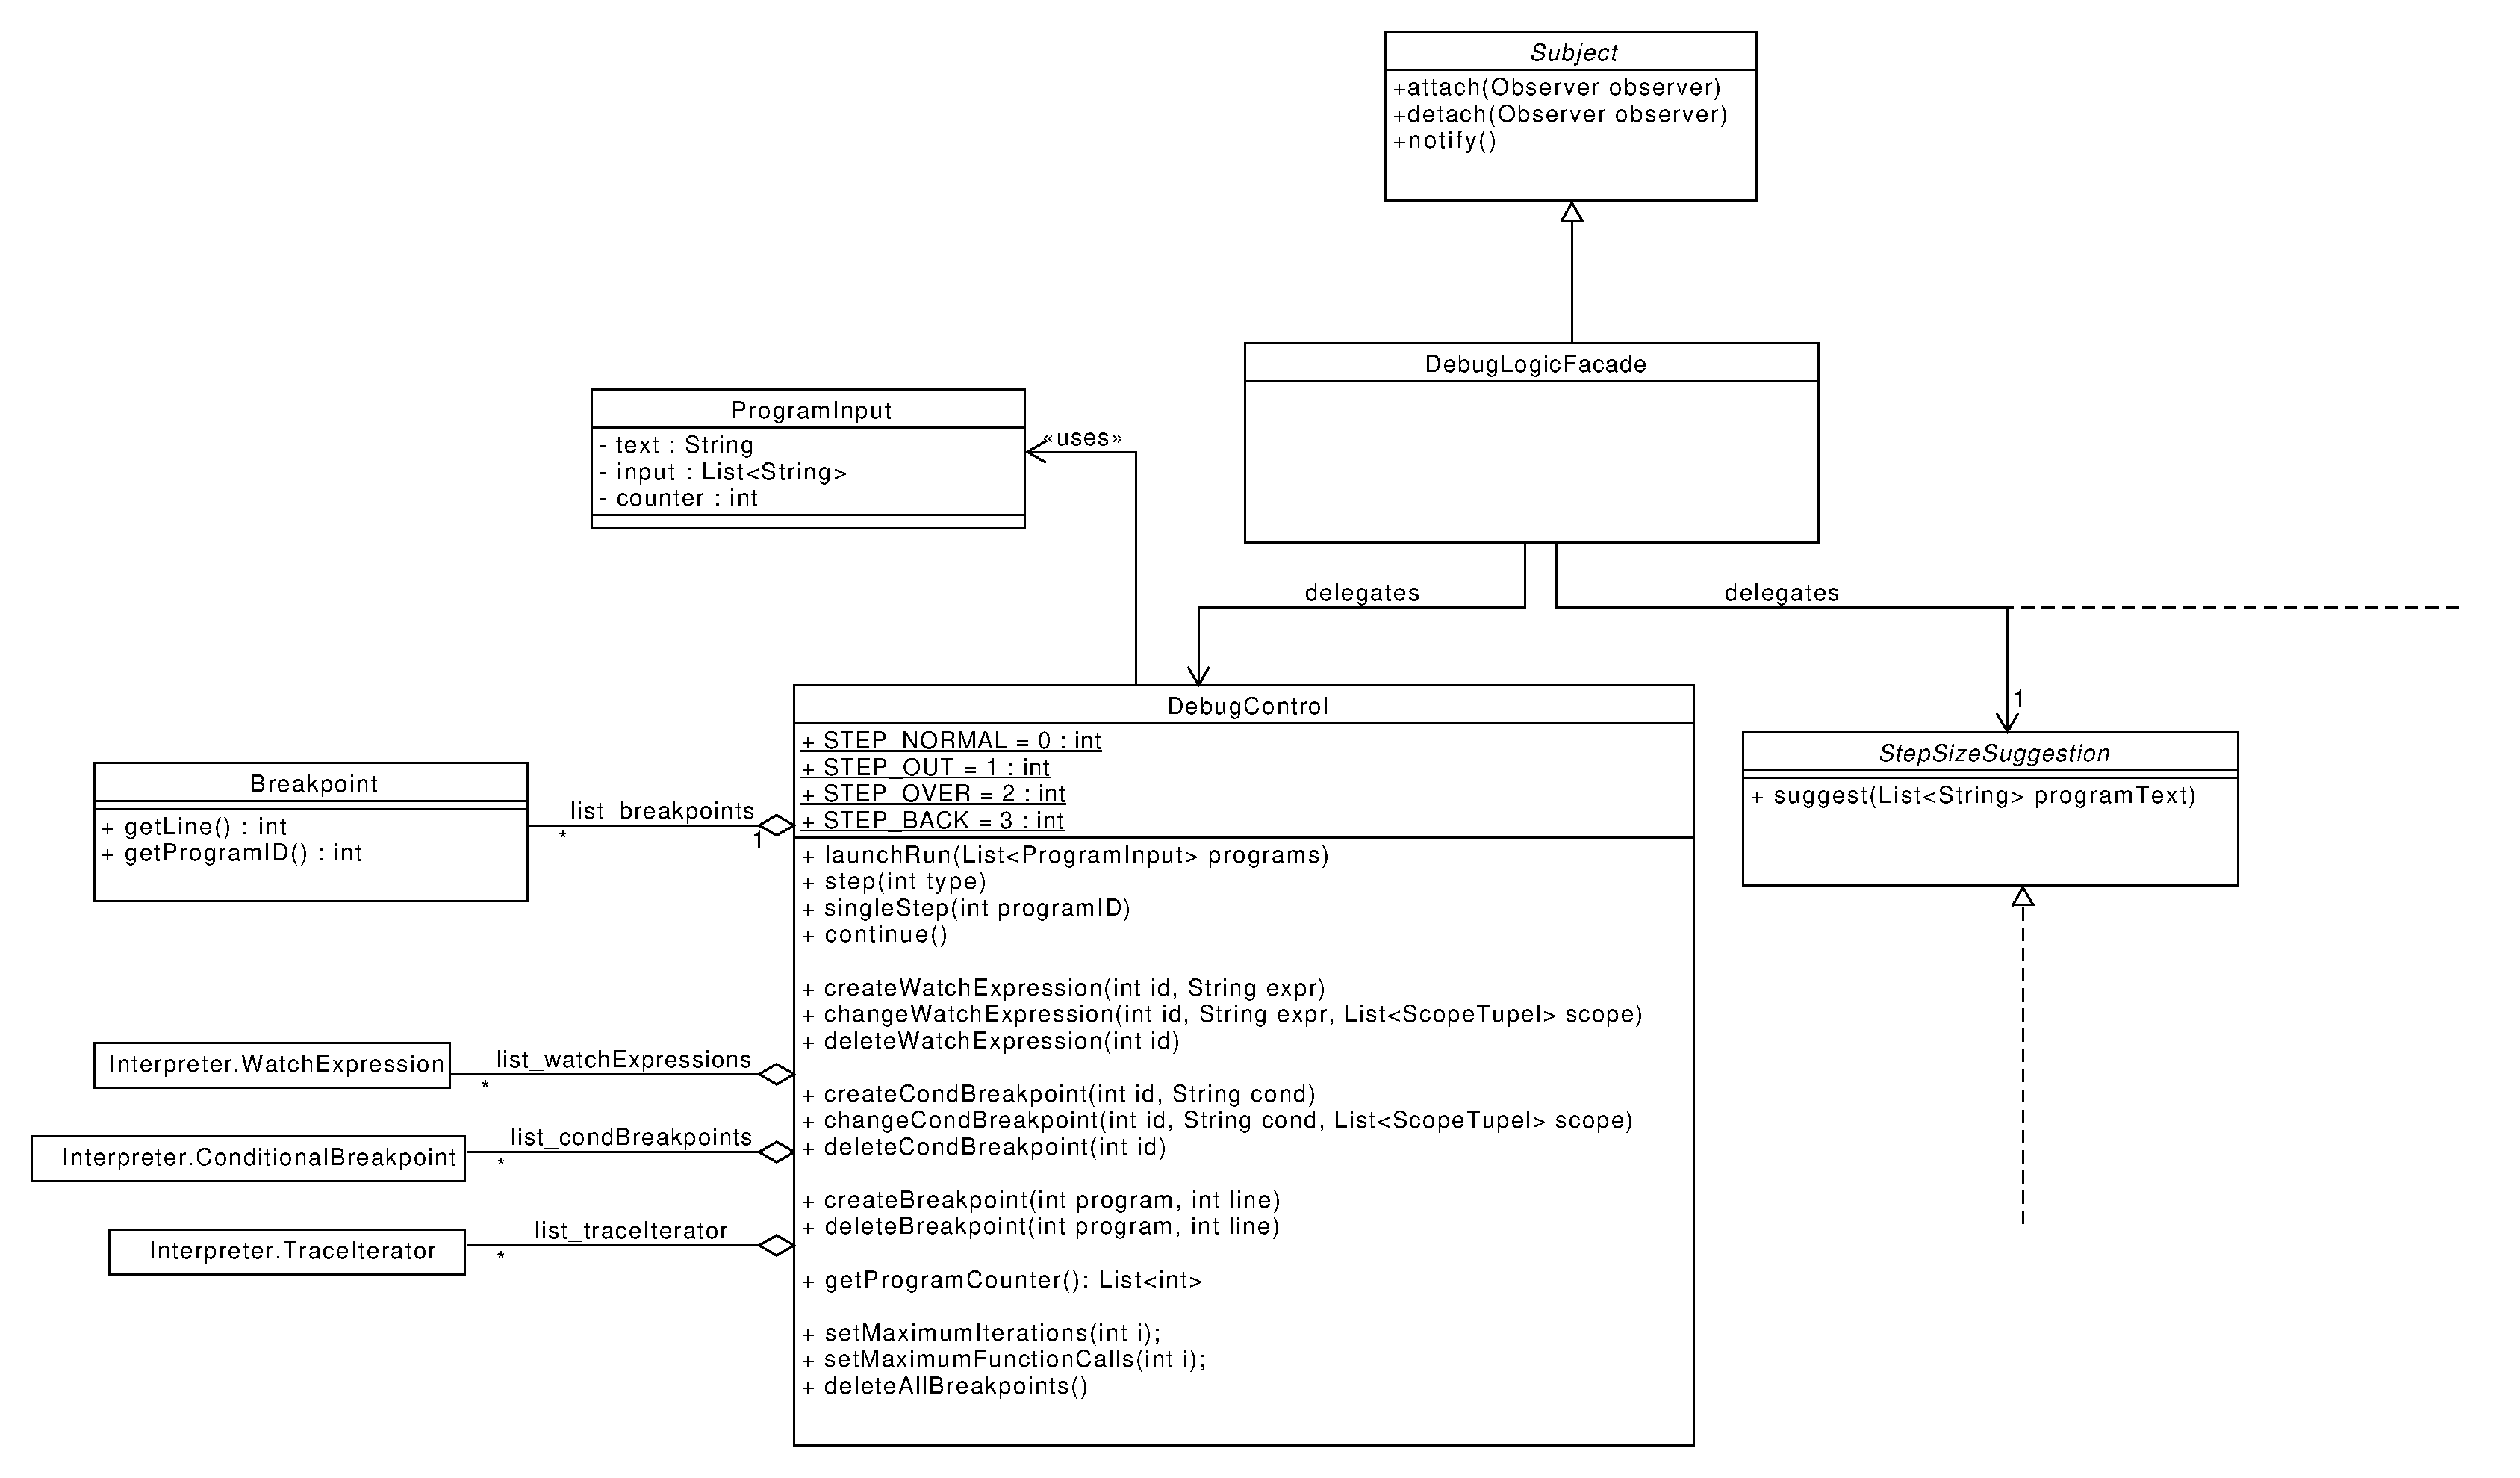
\includegraphics[width=1.2\textwidth]{diagrammIdeenUmlet/DebuggerOverview.pdf}}
\caption{Die Klassen des Paketes \textit{DebugLogic.Debugger}}
\label{fig:debuggerOverview}
\end{figure}
Die Klassenstruktur ist in Abbildung \ref{fig:debuggerOverview} dargestellt.
Die Aktionen des Paketes sind von Anfragen gesteuert, das bedeutet, es geschieht nichts, ohne dass von aussen über die Klasse \textit{DebugLogicFacade} eine entprechende Anweisung als Methodenaufruf kommt. Deshalb hat diese Fassade auch für alle Debugmechanismen entsprechende Methoden, zum Beispiel zur Ausführung von Schritten in den Programmen. \\
Bei jeder Änderung des Zustandes des Debuggers wird nach dem Beobachtermuster die Methode \textit{notify()} der Fassade aufgerufen und so alle Beobachter benachrichtigt.
Je nach Methodenaufruf in der \textit{DebugLogicFacade} wird die Anfrage an die \textit{DebugControl} oder an eine konkrete Ausprägung eines Vorschlagsinterfaces (zum Beispiel \textit{StepsizeSuggestion}) weitergeleitet. Da man das Verfahren, einen solchen Vorschlag zu generieren, beliebig komplex gestalten kann, sollen die verwendeten Algorithmen austauschbar und variabel gehalten werden. Dafür bietet sich das Entwurfsmuster \enquote{Strategie} besonders an. Im Entwurf wird es durch die Interfaces \textit{StepSizeSuggestion, RelationalSuggestion} und \textit{InputValueSuggestion} realisiert. \\
Die konkreten Debugmechanismen werden in der Klasse \textit{DebugControl} gesteuert. So verwaltet diese etwa die vom Paket \textit{DebugLogic.Interpreter} bereitgestellten \textit{WatchExpression}-Instanzen oder die \textit{TraceIterator}-Objekte, um so Schritte auszuführen.
\subsubsection{Wichtige Elemente des Debuggers}
\paragraph{DebugControl}
Die Klasse \textit{DebugControl} koordiniert den Aufruf der Debugmechanismen, wie Start, Schritte, Einzelschritte und Weiter, sowie das Erstellen, Ändern und Löschen von (bedingten) Breakpoints und Watch-Expressions.
\paragraph{ProgramInput}
Kapselt die Informationen zu einem zu debuggenden Programm. Dazu gehören Programmtext, Eingabevariablen und Identifikationsnummer.
\paragraph{Breakpoint}
Kapselt die Informationen eines Breakpoints in einer Zeile eines Programms.
\paragraph{StepsizeSuggestion}
Stellt das Grundgerüst einer Klasse dar (abstrakte Klasse), welche die Größe der Steps anhand der Programmtexte vorschlägt. Durch die Nutzung eines Strategiemusters wird das Erweitern des Produkts durch weitere Arten Vorschläge zu generieren erleichtert.
\paragraph{InputValueSuggestion}
Stellt das Grundgerüst einer Klasse dar (abstrakte Klasse), welche eine Variable eines bestimmtem Typs innerhalb eines Bereichs vorschlägt. Auch hier wird die Erweiterbarkeit des Produkts durch die Nutzung eines Strategiemusters erleichtert.
\paragraph{RelationalSuggestion}
Stellt das Grundgerüst einer Klasse dar (abstrakte Klasse), welche bedingte Breakpoints oder WatchExpressions vorschlägt. Hier wird ebenfalls durch Strategiemuster die Erweiterbarkeit des Produkts um weitere Arten der Vorschlagsgenerierung erleichtert.


\subsection{Interpreter}
\subsubsection{Übersicht}
Dieses Paket ist dafür verantwortlich, die bereits vom \textit{DebugLogic.AntlrParser}  geparsten Nutzereingaben so zu verarbeiten, dass der \textit{DebugLogic.Debugger} damit weiterarbeiten kann. Nimmt das Paket vom \textit{DebugLogic.AntlrParser} den Quelltext eines (WLang-) Programms entgegen, erzeugt es einen Pfad über den gesamten Programmfluss des Programms, sodass später darüber iteriert werden kann. Nimmt das Paket Zeichenketten entgegen, die Watch-Expressions und bedingte Breakpoints beschreiben, interpretiert diese und stellt sie abstrakt dar.
Innerhalb dieses Paketes wird auch auf semantische Fehler geprüft, etwa das Fehlen eines return-Statements.\\
Dieses Unterpaket benutzt das Unterpaket \textit{DebugLogic.AntlrParser}, um damit aus den reinen Zeichenketten einen Syntaxbaum gemäß der im Anhang \ref{Anhang} gegebenen Grammatik für die Sprache WLang erzeugen zu lassen.
Der Vorgang der Erzeugung des oben erwähnten Pfades wird genauer in \ref{TraceGen} erklärt.
\subsubsection{Wichtige Elemente des Interpreters}
\paragraph{GenerationController}
Steuert die Erzeugung eines kompletten Programmverlaufs (Trace), siehe Kapitel \ref{charAbl}.
\paragraph{CommandGenerationVisitor}
Verwendet das Visitor Entwurfsmuster, um über einen Ableitungsbaum nach der in Kapitel \ref{FormSpez} gegebenen WLang-Grammatik zu gehen und dabei eine Menge von Commands zu erzeugen. \\
Um die Term- und Befehlsstrukturen zu erzeugen, wird  hier das Entwurfsmuster \textit{Visitor} verwendet. Zum einen ermöglicht es, die von Antlr generierten \textit{ParseTree}-Objekte mit den von Antlr vorgegebenen Schnittstellen zu durchlaufen. Zum anderen bietet dieses Pattern die Möglichkeit, beliebige Operationen auf den Ableitungsbäumen auszuführen, ohne die von Antlr generierten Klassenstrukturen zu verändern. Die Nutzung dieses Patterns ist daher beim Umgang mit Antlr beinahe unumgänglich.
\paragraph{Scope}
Kapselt aktuelle Variablenbelegung innerhalb eines Funktionsaufrufs.
\paragraph{Command}
Stellt einen ausführbaren Befehl dar, der die aktuellen Variablenzustände gemäß seiner Semantik verändern kann.
\\
Für diese Klasse und ihre Unterklassen wird ein \enquote{Kompositum} verwendet.
Ein Auszug davon ist in Abbildung \ref{Command} zu sehen. Zunächst gibt es elementare Befehle, wie etwa eine einfache Zuweisung. Es gibt jedoch auch Befehle, wie etwa while- und if- Befehle, die mehrere Unterbefehle haben, und entscheiden müssen, ob und wie oft diese ausgeführt werden. Sie stellen also in diesem Fall Befehlskompositionen dar. Ein großer Vorteil dieser Modellierung besteht in der Nutzung der Methode \textit{run()}. Der Aufrufer eines Befehls muss nicht wissen, ob es sich um einen elementaren Zuweisungs- oder Deklarationsbefehl oder um einen komplexen zusammengesetzten Befehl wie etwa eine Schleife handelt. Ihn interessiert nur die während der Ausführung des Befehls angenommenen Zustände. Die Befehlsfunktionalität wird so weggekapselt. \\
Einen Befehl als Objekt zu kapseln, um diesen in Warteschlangen zu fügen, aufzubewahren oder Empfänger damit zu parametrisieren ist der Zweck des Entwurfsmusters \enquote{Command}, das hier auch verwendet ist. Da die Befehle zunächst alle erzeugt und dann später ausgeführt werden. Die Ausführung der Befehle ist entsprechend komplex, da dabei etwa Typprüfungen stattfinden müssen (Näheres dazu ist in Kapitel \ref{charAbl} zu finden), weswegen es sich auch empfiehlt, diese Arbeit zu kapseln. 
\begin{figure}[!h]
\centering
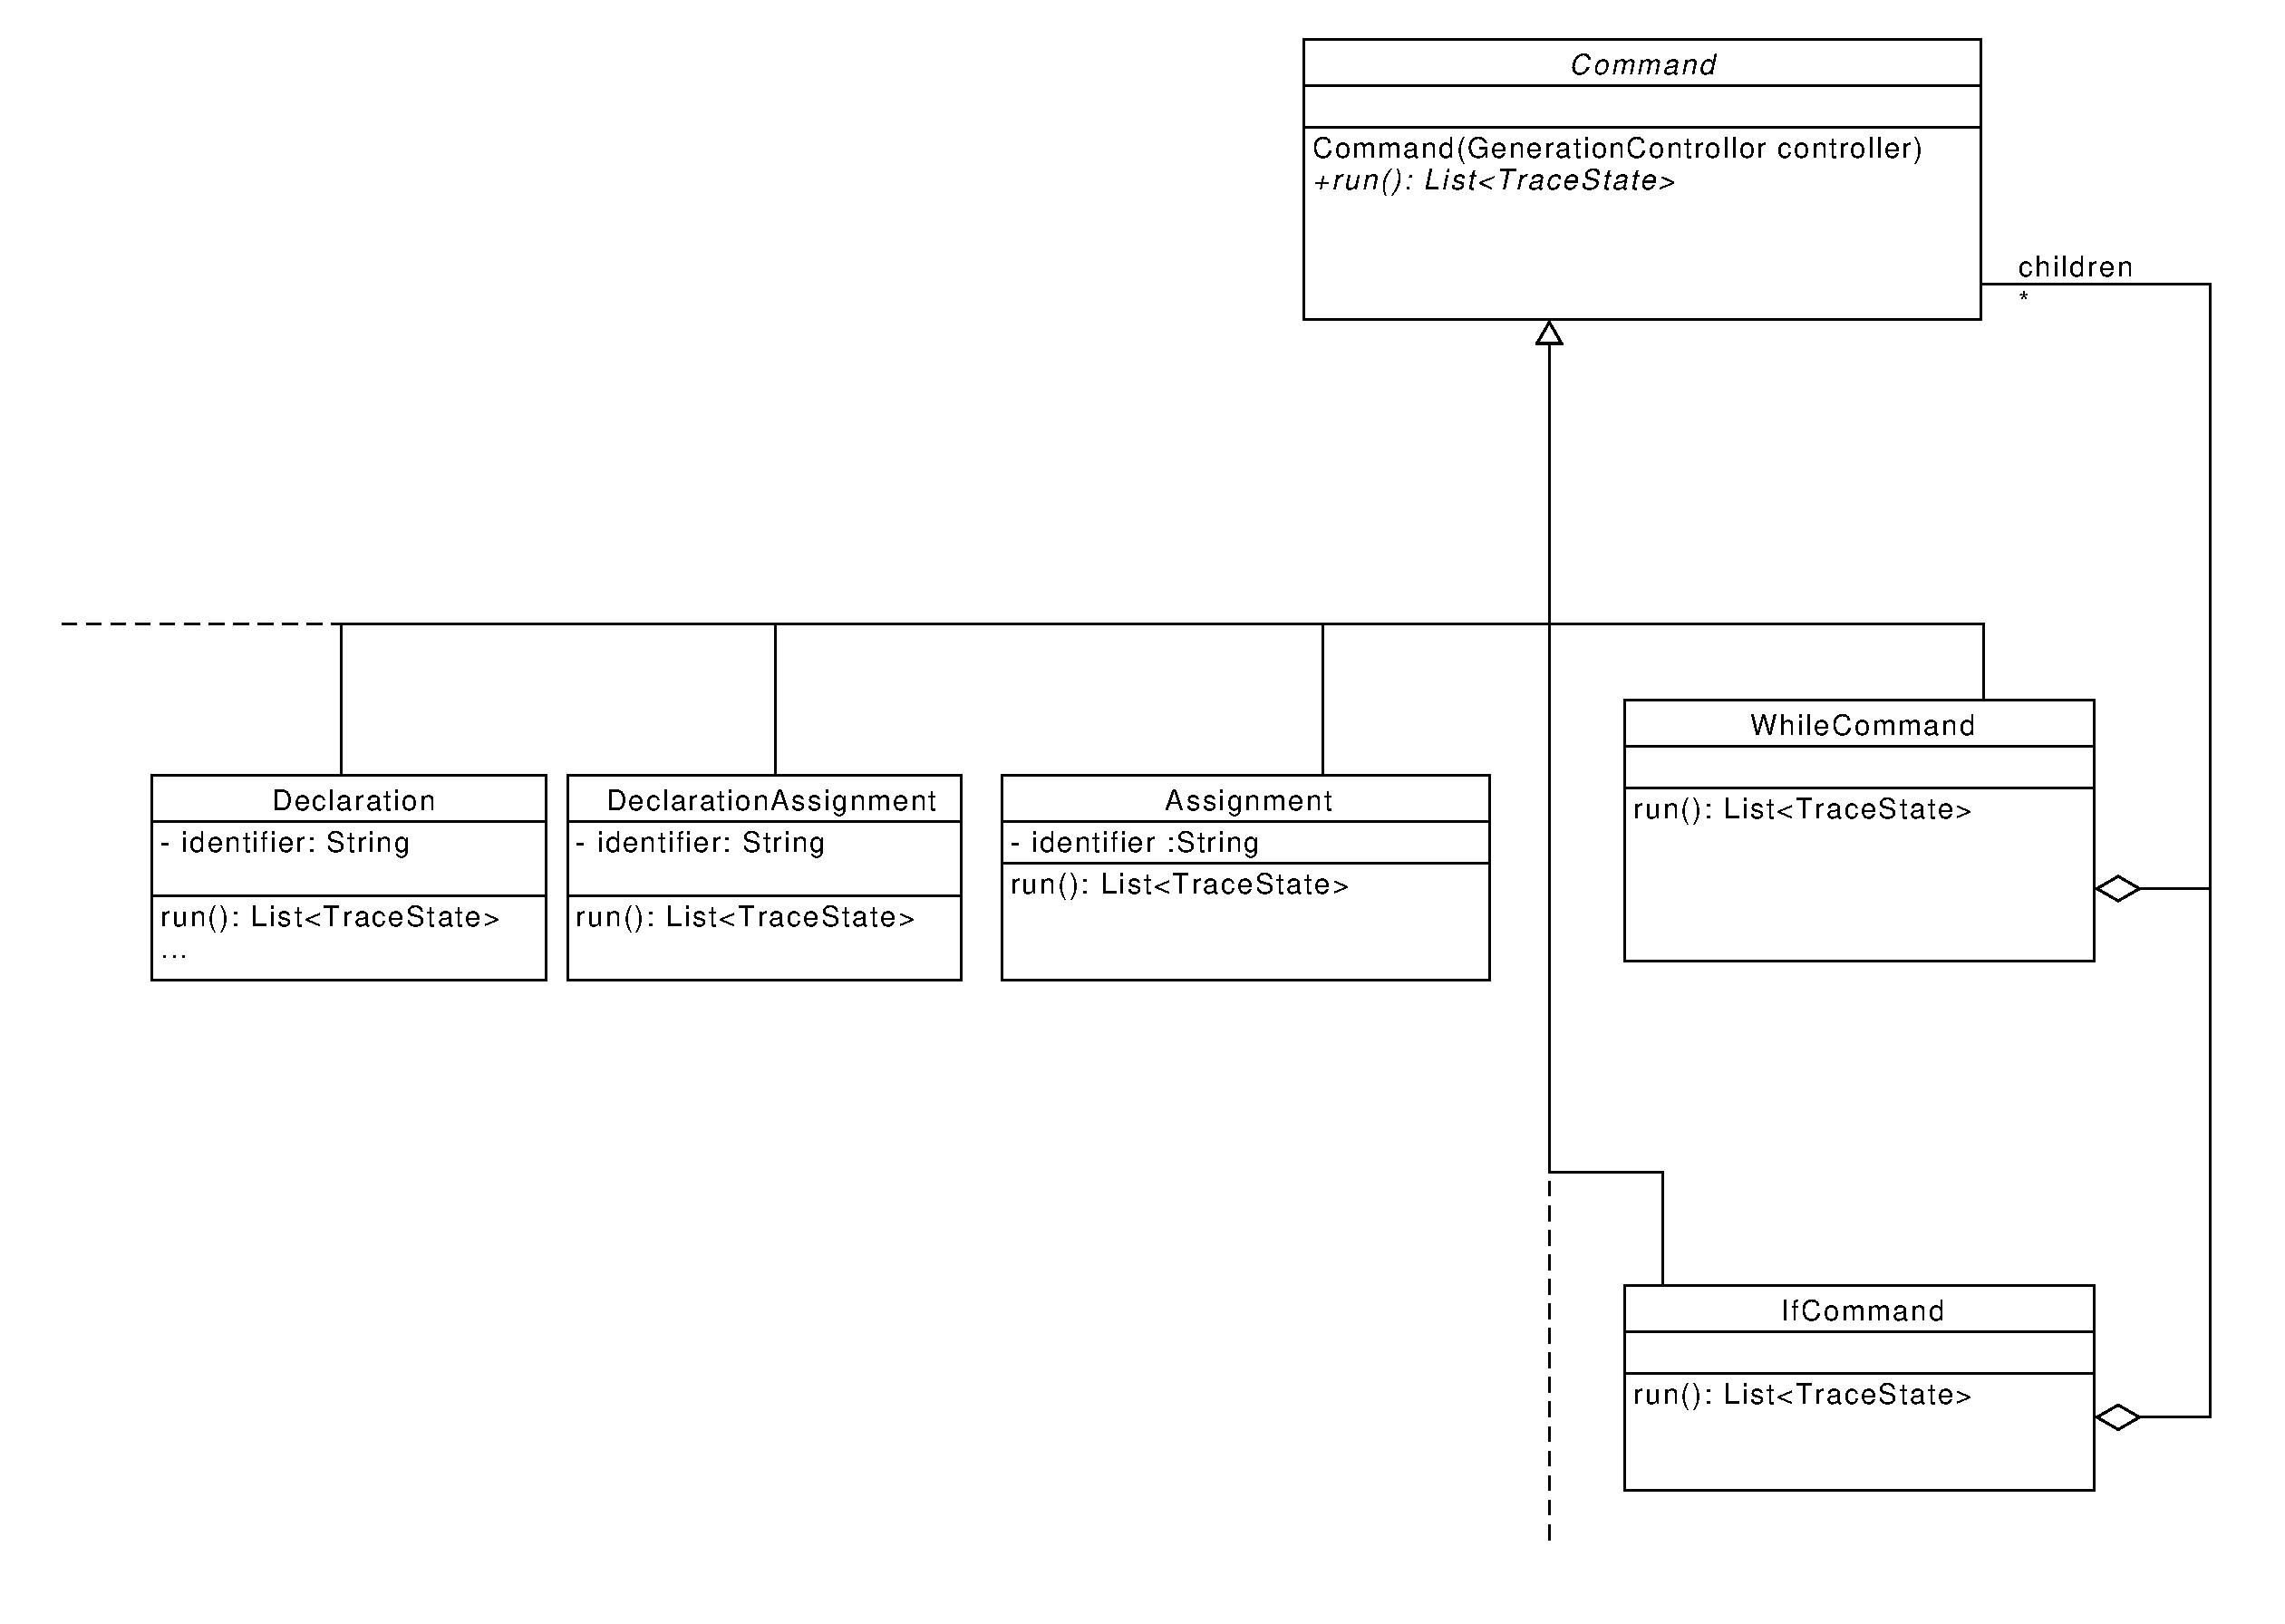
\includegraphics[width=1.0\textwidth]{diagrammIdeenUmlet/CommandComposite.pdf}
\caption{Die Klasse \textit{Command} als Kompositum}
\label{Command}
\end{figure}
\paragraph{Trace}
Stellt den kompletten Programmverlauf eines WLang-Programms dar.
\paragraph{TraceState}
Stellt einen Zustand während des Programmverlaufs eines WLang-Programms dar.
\paragraph{Der Traceiterator}
\begin{figure}[!h]
\centering
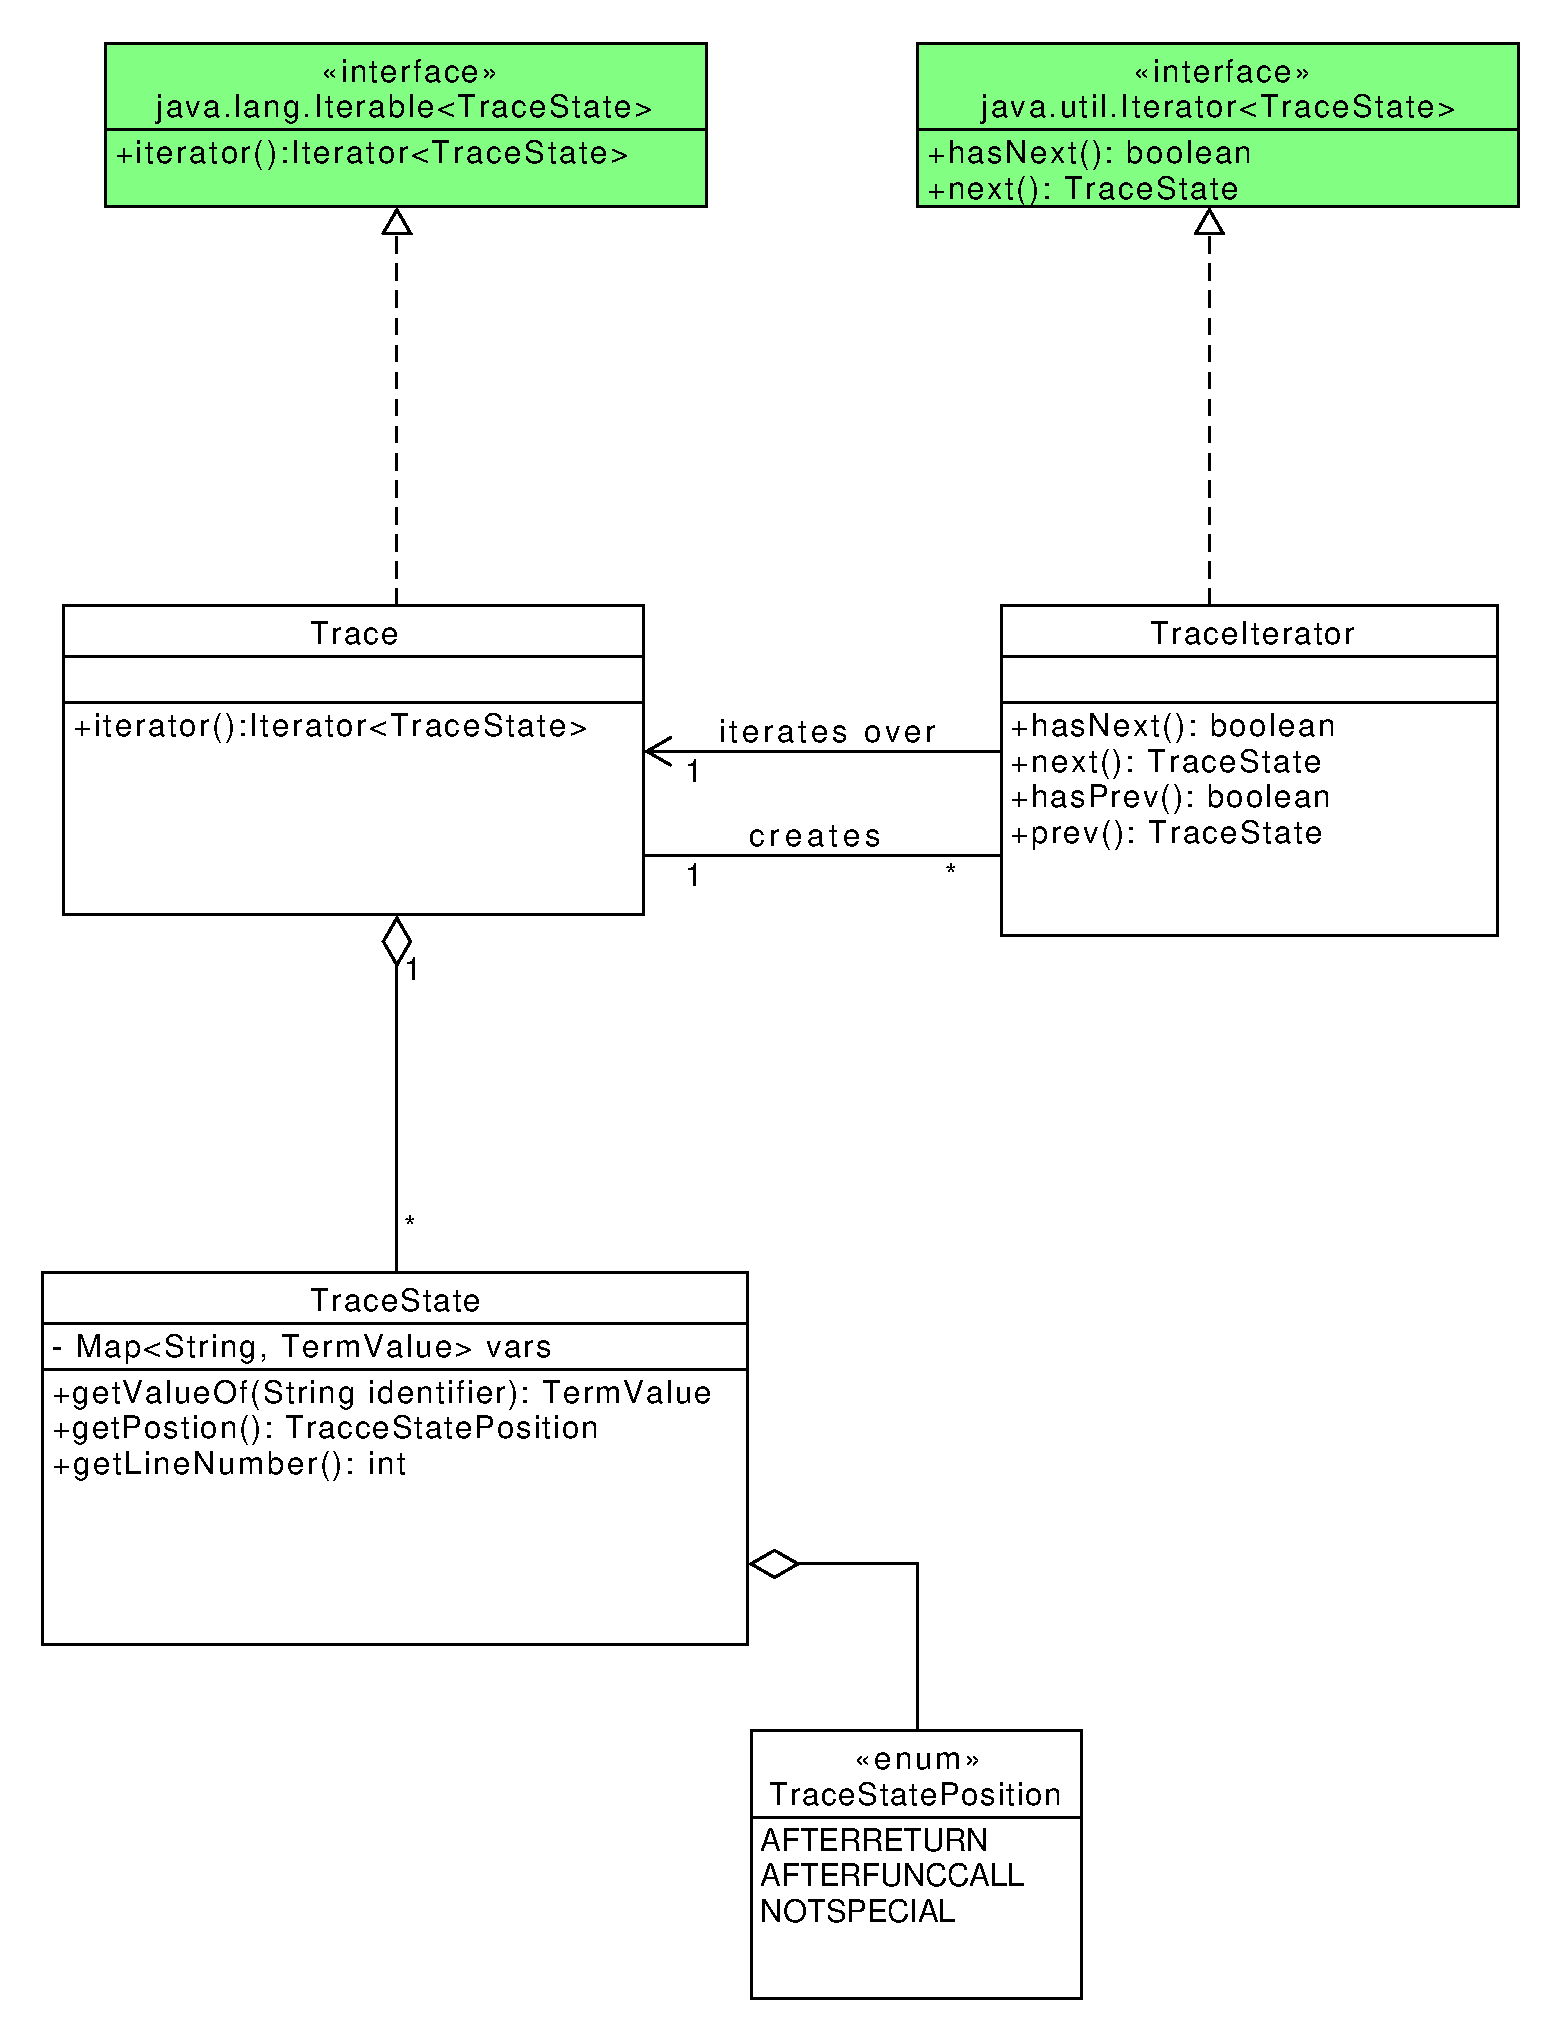
\includegraphics[width=0.8\textwidth]{diagrammIdeenUmlet/TraceIteratorPattern.pdf}
\caption{Der Traceiterator}
\label{TraceIterator}
\end{figure}
Wir betrachten Abbildung \ref{TraceIterator}.
Grundkonzept des Debuggens ist die folgende Idee: Zunächst wird die komplette Ausführung eines Programmlaufes berechnet und dabei nach jedem ausgeführten Befehl der Zustand der Variablen gespeichert. Die Aggregation all dieser als \textit{TraceState}-Instanzen dargestellten Zustände ist ein sogenanntes \textit{Trace}-Objekt. Um es dem Paket \textit{DebugLogic.Debugger} zu ermöglichen, ohne Kenntnis der konkreten Darstellung dieses Traces über die \textit{TraceState}-Objekte zu iterieren, wird lediglich ein \textit{TraceIterator}-Objekt nach außen gegeben. Um dabei die volle von Java angebotene Funktionalität zu nutzen, werden die entsprechenden Java Schnittstellen implementiert. 
\paragraph{Term}
Stellt eine Abstrakte Repräsentation eines arithmetischen bzw. logischen Terms dar. 
\\
Die Struktur eines Termes kann wie folgt beschrieben werden: \\
Konstanten und Variablen sind Terme. Sind $A$ und $B$ Terme und $\sigma$ ein zweistelliger Operator, dann ist auch $A\sigma B$ ein Term. Ist $\nabla$ ein einstelliger Operator, dann ist auch $\nabla A$ ein Term. Diese induktiv aufgebaute Struktur der Terme lässt sich in naheliegender Weise in eine Klassenstruktur übertragen, die in Abbildung \ref{Terme} dargestellt ist. Hier wird das Entwurfsmuster \enquote{Kompositum} verwendet. Der Vorteil besteht in der einfachen und einheitlichen Nutzung der Funktion \textit{evaluate()}. Diese gibt eine Instanz vom Typ \textit{TermValue} zurück. Die vollständige Funktionalität des vorliegenden Typsystems ist in den Implementierungen dieser Schnittstelle gekapselt. Einen Spezialfall von Termen stellen \textit{BinaryCondition} und \textit{Comparison} dar. Diese werten sich per Definition zu booleschen Werten aus. Das Liskovsche Substitutionsprinzip erlaubt Kovarianz in den Ausgabeparametern, weswegen es möglich ist, diesen Subklassen von \textit{Term} in den \textit{evaluate()}-Methoden den Rückgabetyp \textit{BooleanValue} zu geben, eine spezielle Implementierung des \textit{TermValue}-Interfaces.
\begin{center}
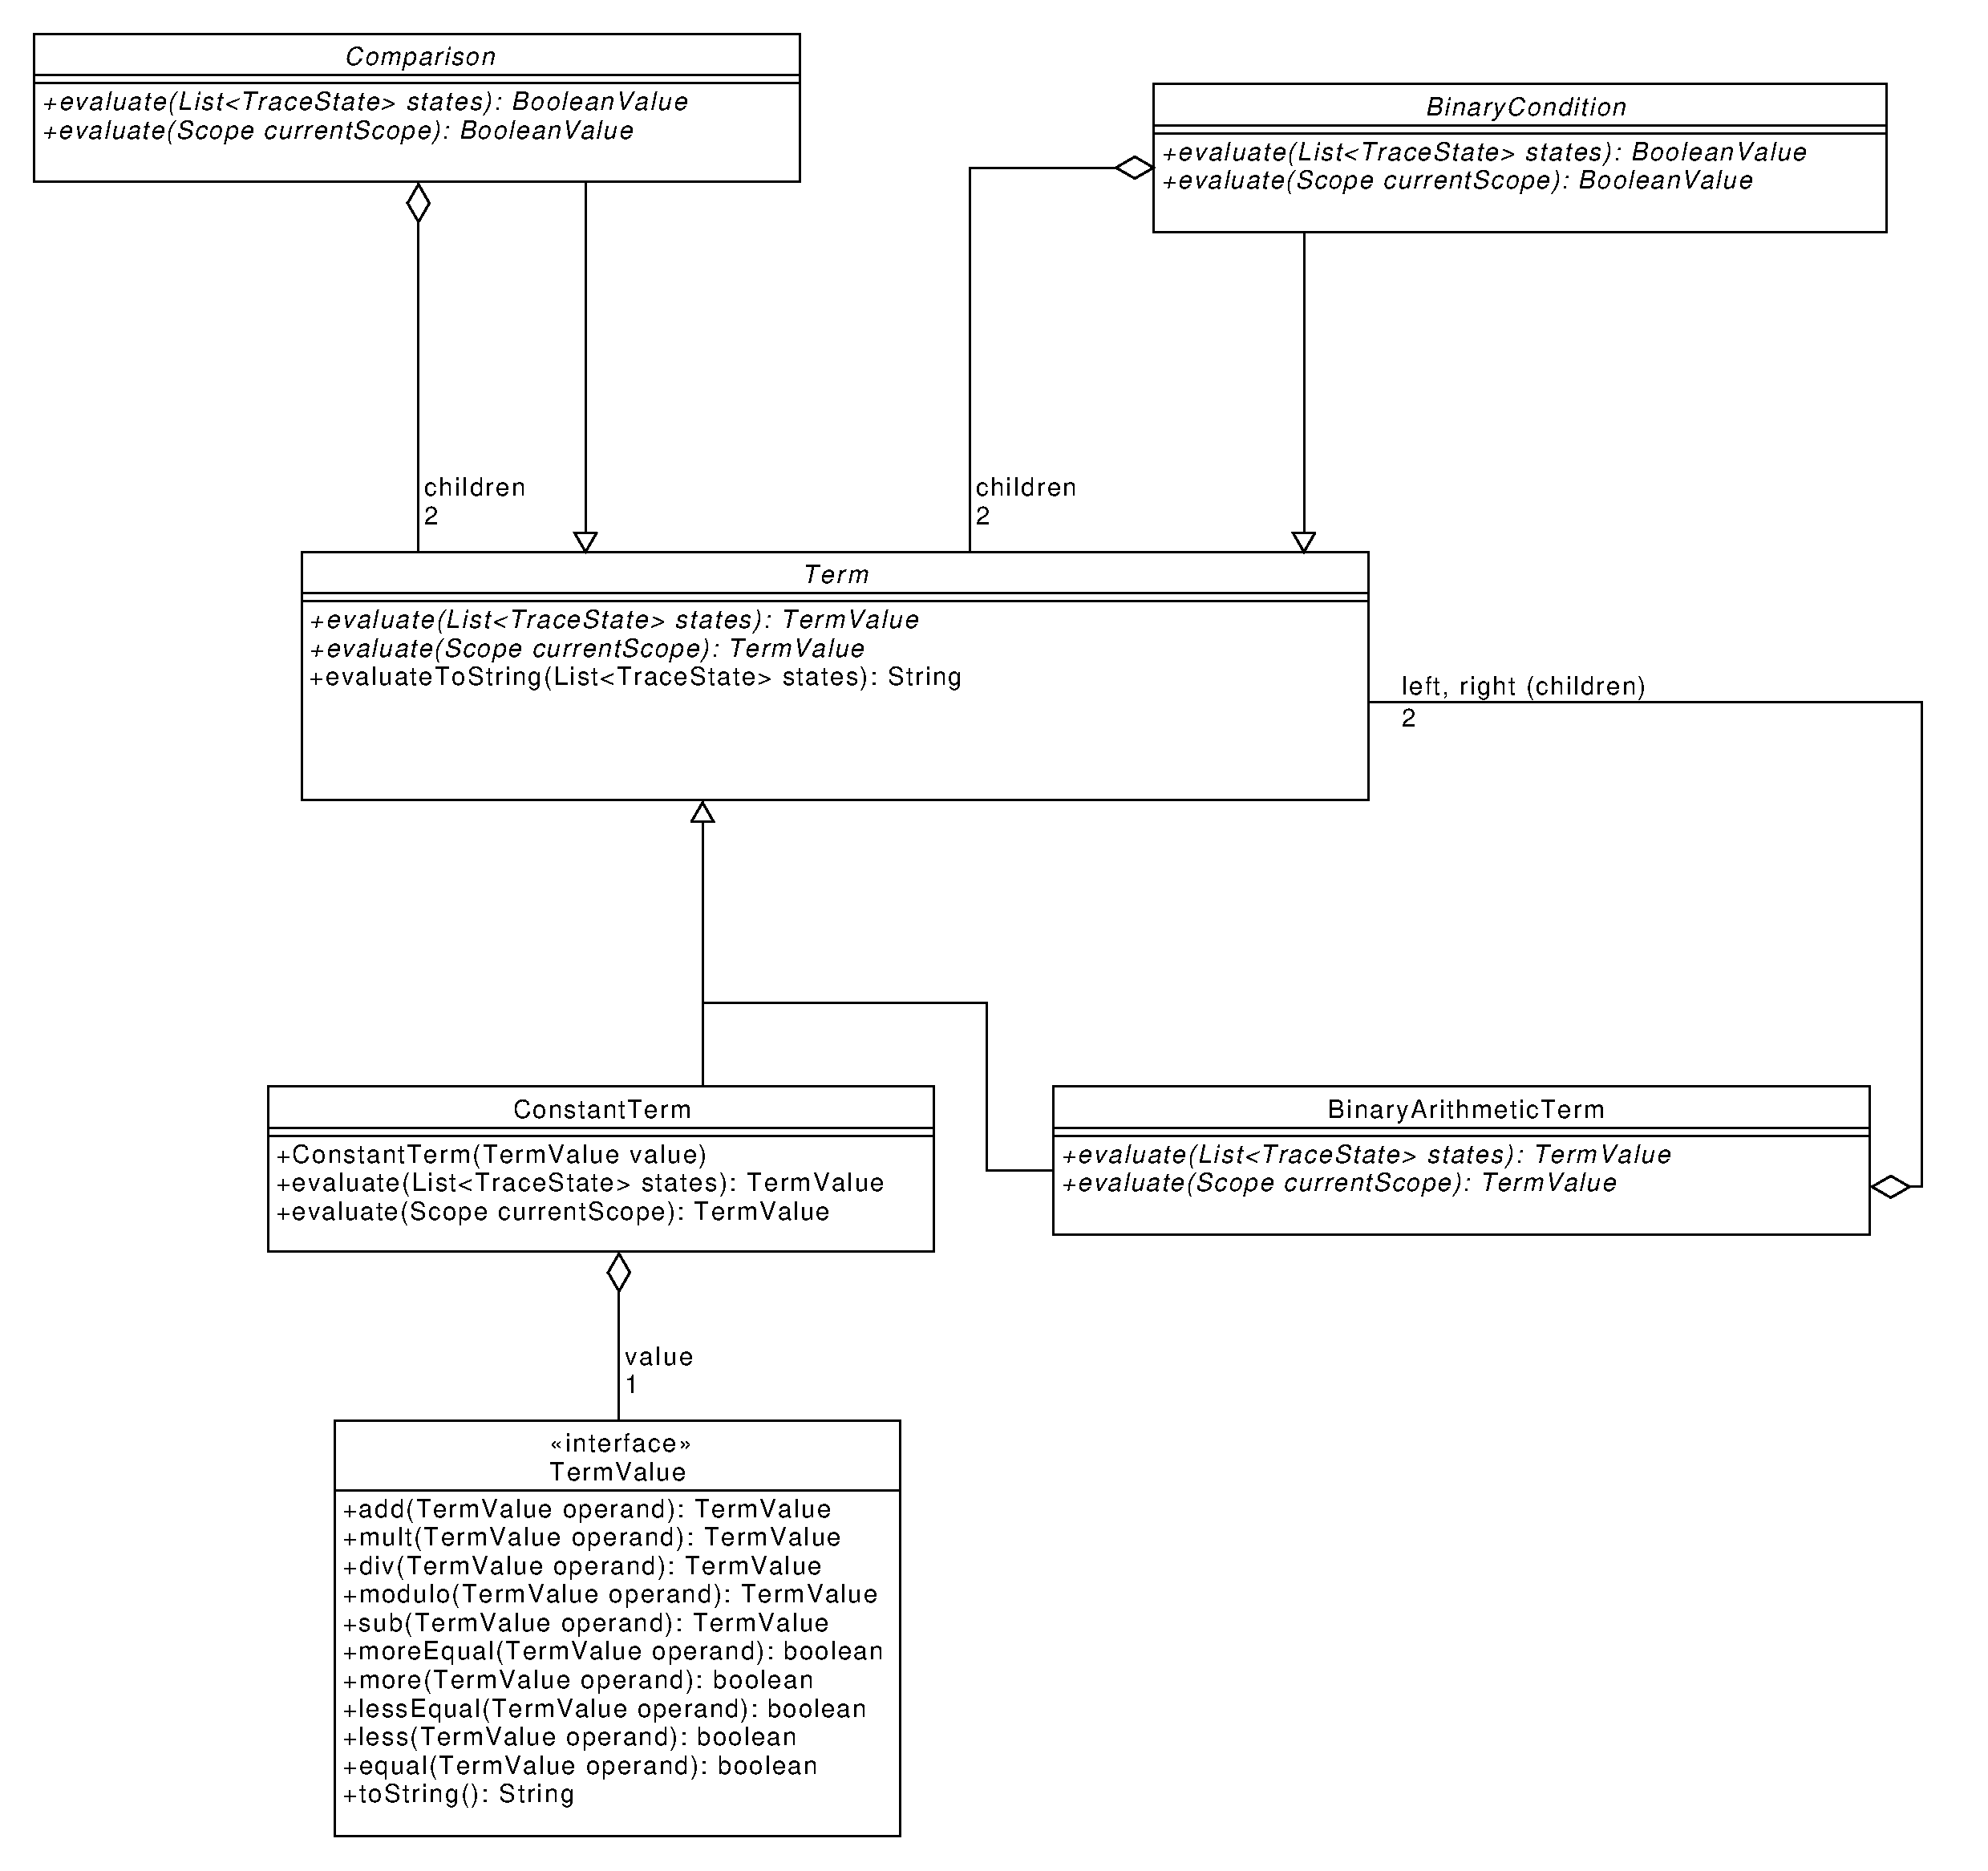
\includegraphics[width=1.0\textwidth]{diagrammIdeenUmlet/TermCondition.pdf}
\captionof{figure}{Das Termkompositum im Entwurf}
\label{Terme}
\end{center}
\paragraph{WatchExpression}
Diese Klasse repräsentiert eine Watch-Expression, welche ein Ausdruck über den Variablen verschiedener Programme ist, der sich innerhalb seines Gültigkeitsbereiches zu einem bestimmten Wert auswertet.
\paragraph{ConditionalBreakpoint}
Ein Conditional Breakpoint ist ein Ausdruck über den Variablen verschiedener Programme, der sich innerhalb seines Gültigkeitsbereiches zu einem booleschen Wert auswertet.

\subsection{Antlr Parser}
Dieses Paket beinhaltet nur Klassen, welche von der Antlr Bibliothek auf Basis der WLang Grammatik generiert werden und somit nicht per Hand geschrieben sind. \\
Dieses Unterpaket parst die Eingaben des Nutzers (d.h. sowohl Programmtexte als auch Variablen und Ausdrücke für bedingte Breakpoints und Watch-Expressions) gemäß der im Anhang (Kapitel \ref{Anhang})  gegebenen Grammatik. Genauer wird die Verwendung des Antlr Parsers in Kapitel \ref{FormSpez} beschrieben.

\subsection{Exceptions}
\subsubsection{Übersicht}
Dieses Unterpaket enthält Klassen, die, für das Produkt spezifisch entwickelte, Exceptions darstellen. Um das Handling dieser Exceptions kümmert sich die \textit{Control}.
\subsubsection{Wichtige Elemente des Exception-Unterpakets}
\paragraph{DIbuggerLogicException}
Dieses Interface sorgt dafür, dass alle Klassen in diesem Paket, die notwendigen Methoden implementieren.
Alle Klassen in diesem Paket implementieren diese Schnittstelle. 
%die folgenden Exceptions beziehen sich auf semantisch fehlerhafte eingegebene (WLang-)Programme.
\paragraph{MissingReturnCallException}
Ausnahme, die ausgelöst wird, falls eine Methode in WLang einen Rückgabewert verlangt aber kein return Statement enthält.
\paragraph{InvalidProgramException}
Ausnahme, die ausgelöst wird, falls eine Programmdatei nicht korrekt ist oder das eingegebene Programm nicht dem Standard von WLang entspricht
\paragraph{WrongArgumentException}
Abstrakte Klasse und Ausnahme, die bei falscher Eingabe der Parameter ausgelöst wird. Das UML-Diagramm stellt die Unterklassen dieser abstrakten Klasse dar.
%TODO UML Diagramm
\paragraph{ReturnTypeException}
Ausnahme, die ausgelöst wird, wenn in einer Methode ein falscher Rückgabewert (Typ) zurückgegeben wird.
\paragraph{WrongTypeAssignmentException}
Ausnahme, die ausgelöst wird, falls in einer Zuweisung die Typen von Zielvariable und neuem Wert nicht kompatibel sind.
\paragraph{VariableNotFoundException}
Ausnahme, die ausgelöst wird, falls eine Variable nicht vorhanden ist und darauf zugegriffen wird.
\paragraph{AlreadyDeclaredException}
Ausnahme, die ausgelöst wird, falls eine Variable bereits deklariert wurde und versucht wird, dies zu wiederholen
\paragraph{RoutineNotFoundException}
Ausnahme, die ausgelöst wird, falls eine Methode/Funktion aufgerufen wird, welche nicht existiert


\newpage
\section{Charakteristische Abläufe}\label{charAbl}
In diesem Kapitel werden charakteristische Abläufe des Produkts, wie der erste Programmaufruf und die
Anwendungsfälle, anhand von Sequenzdiagrammen dargestellt und erklärt.
 %TODO Auf Klassen oder Pakete in Beschreibung aller Klassen verweisen

\subsection{Erster Programmaufruf}
\begin{center}
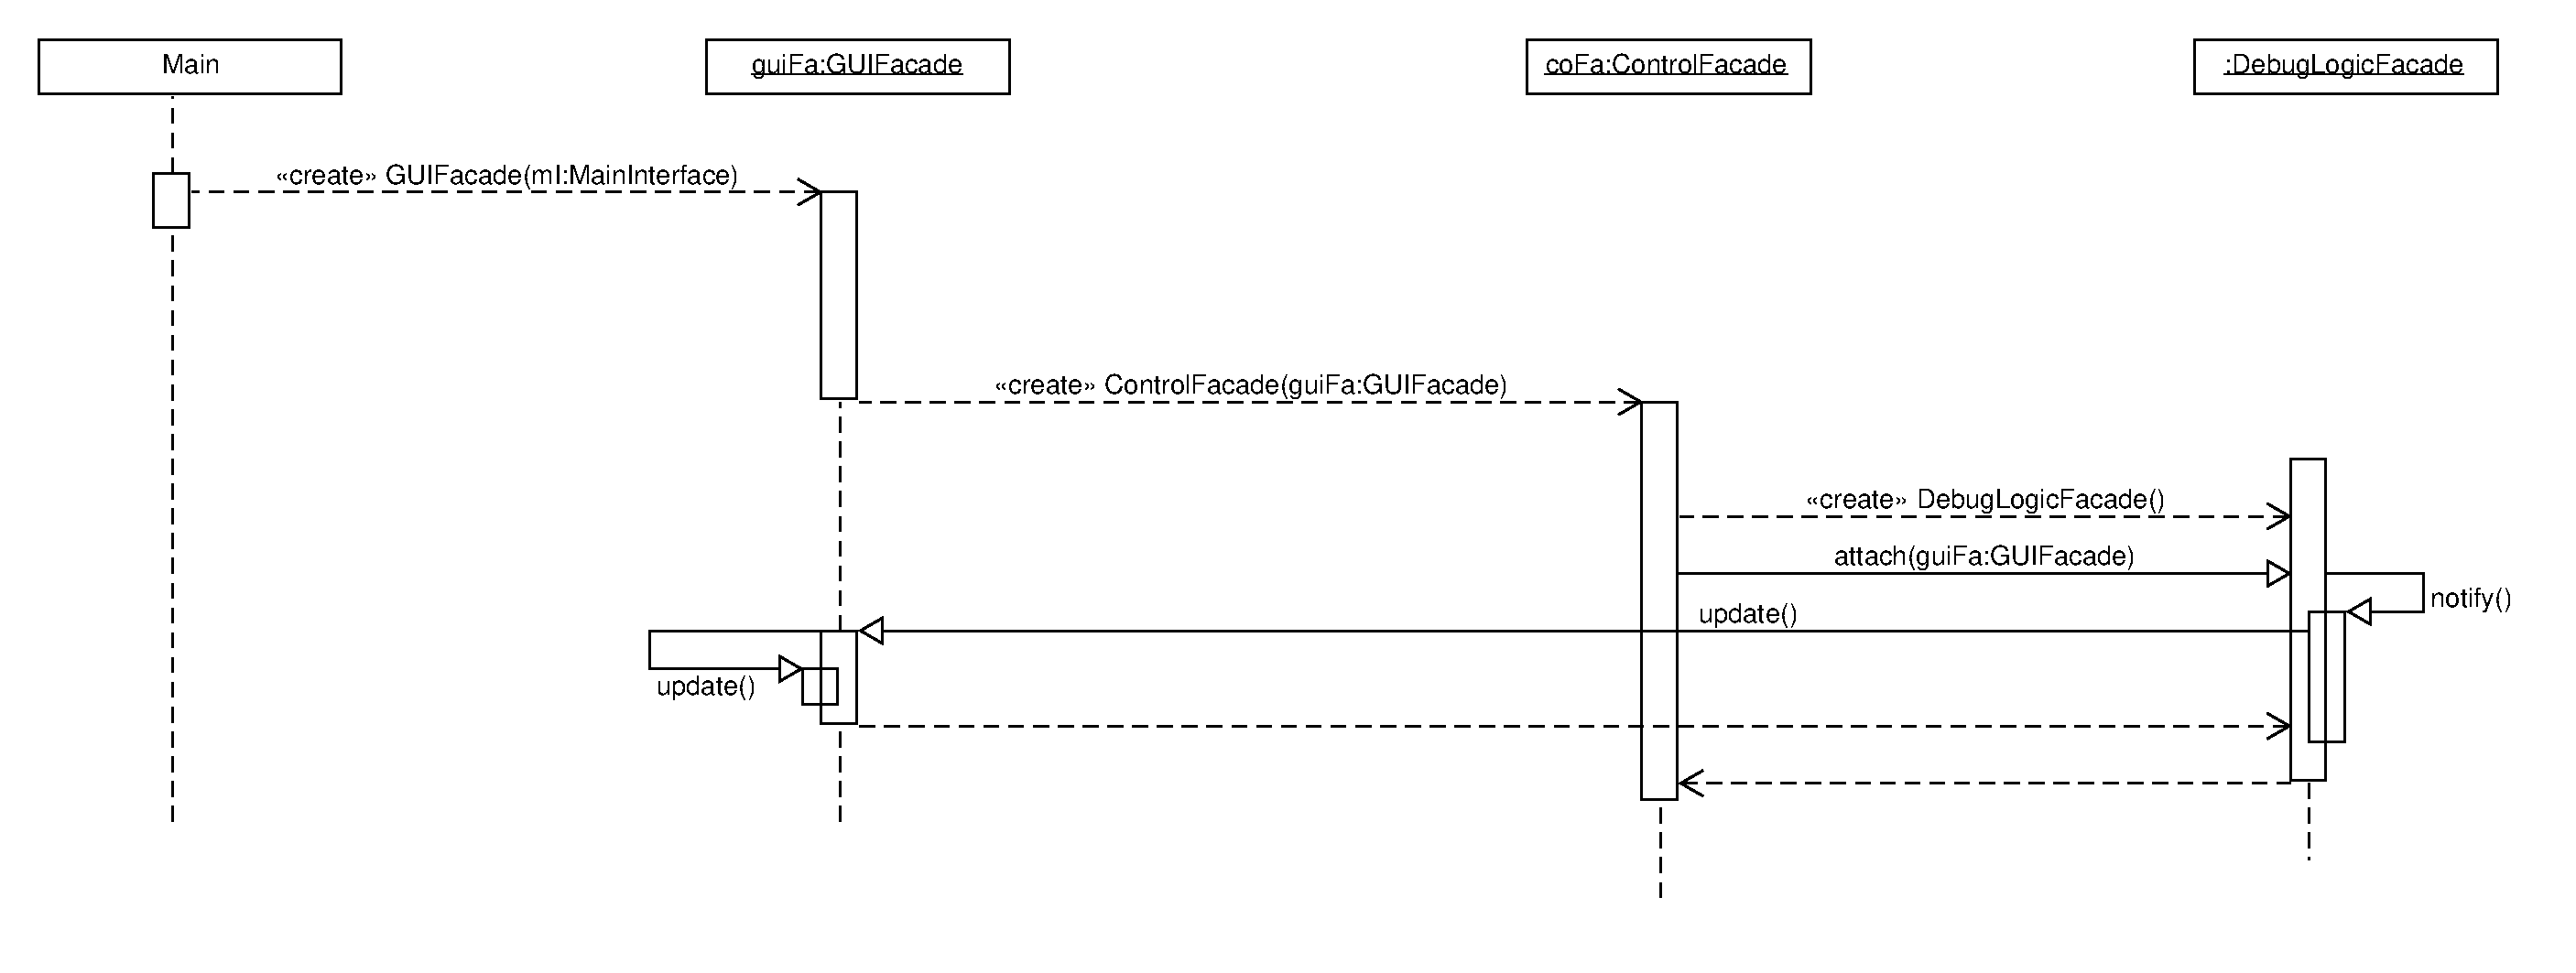
\includegraphics[width=1.0\textwidth]{diagrammIdeenUmlet/SequenceDiagrams/seq_firstCallPDF.pdf}
\captionof{figure}{Sequenzdiagramm: Erster Programmaufruf}
\end{center}
Wird das Produkt gestartet, erstellt die Main-Methode des MainInterface die GUIFacade und übergibt sich selbst.
Die GUIFacade speichert das MainInterface und erstellt ihrerseits die ControlFacade, welche wiederum
die DebugLogicFacade erstellt.
Die ControlFacade und DebugLogicFacade erstellen intern Instanzen der Klassen ihrer Pakete. \\
Die GUIFacade wird bei diesem Prozess bis zur DebugLogic weitergereicht, um dort als Observer angemeldet werden
zu können. Wird später dann zum Beispiel ein Breakpoint hinzugefügt, wird die GUIFacade benachrichtigt und
kann sich updaten.

\newpage
\subsection{Konfigurationsdatei laden}
\begin{center}
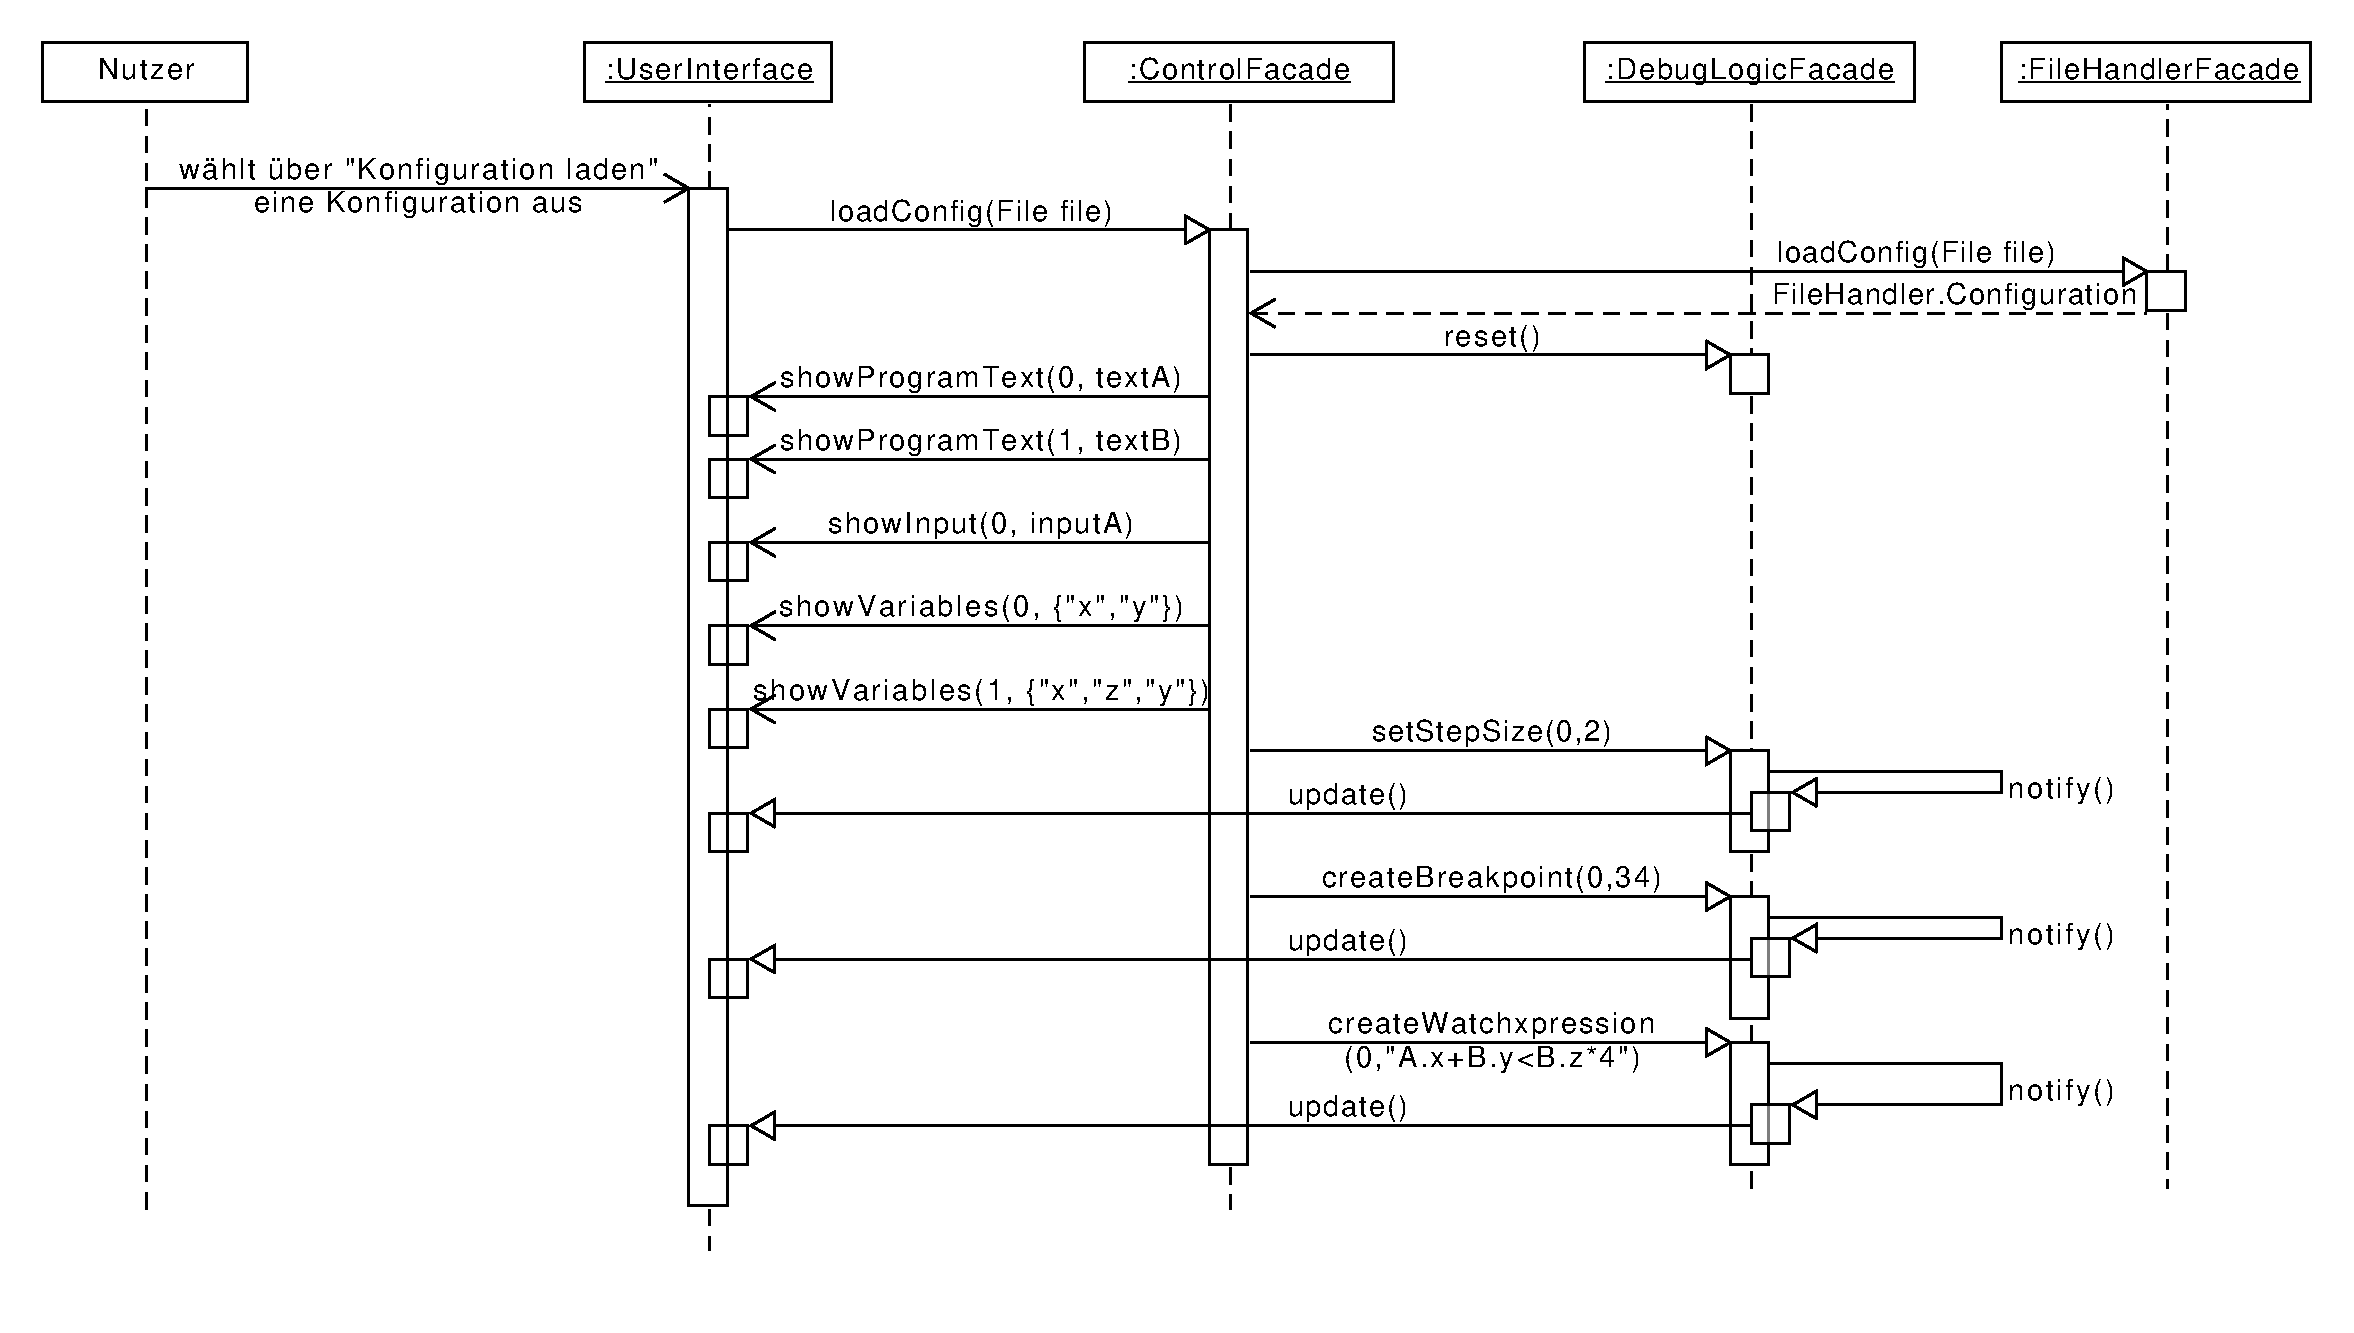
\includegraphics[width=1.0\textwidth]{diagrammIdeenUmlet/SequenceDiagrams/seq_loadConfigPDF.pdf}
\captionof{figure}{Sequenzdiagramm:  Laden einer Konfigurationsdatei}
\end{center}
Wählt der Benutzer über den Menüeintrag \enquote{Konfigurationsdatei laden} eine Konfiguration aus,
gibt das UserInterface diesen Befehl an die Control weiter, welche ein Configuration Objekt vom FileHandler 
erhält. \\
Die Control ruft anschließend Methoden der GUIFacade auf, um die Programmtexte, Eingabevariablen und
die im Variableninspektor anzuzeigende Variablen anzuzeigen. Außerdem ruft die Control
Methoden der DebugLogicFacade auf, um für jedes Programm die Breakpoints, Watch-Expressions und
Schrittgrößen festzulegen. Über diese Änderungen wird das UserInterface als Observer benachrichtigt und kann diese ebenfalls anzeigen.

\newpage
\subsection{FA140: Konfigurationsdatei speichern}
\begin{center}
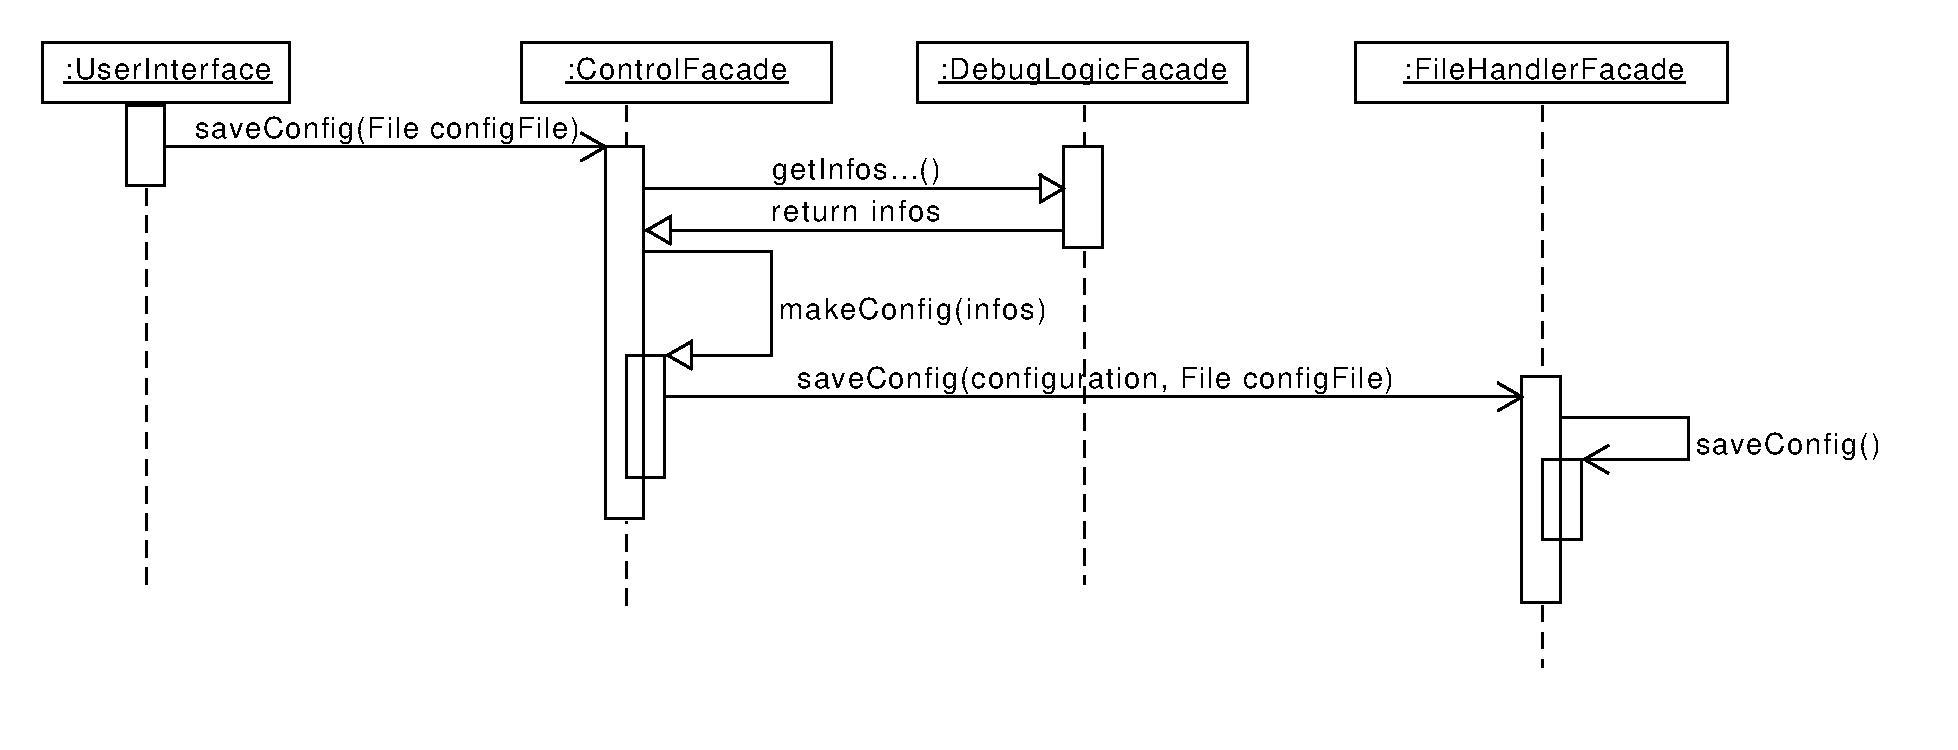
\includegraphics[width=1.0\textwidth]{diagrammIdeenUmlet/SequenceDiagrams/seq_saveConfigPDF.pdf}
\captionof{figure}{Sequenzdigramm: Speichern einer Konfigurationsdatei}
\end{center}
Möchte der Benutzer eine Konfigurationsdatei speichern, reicht das UserInterface den Speicherort
an die ControlFacade weiter. Die Control sammelt die benötigten Daten in einer Configuration Instanz.
Dieses Objekt wird mit dem angegebenen Speicherort an die FileHandlerFacade weitergegeben, welche 
dann die Konfigurationsdatei auf dem Rechner des Benutzers speichert.

\newpage
\subsection{AF10: Hinzufügen von Programmen}
\begin{center}
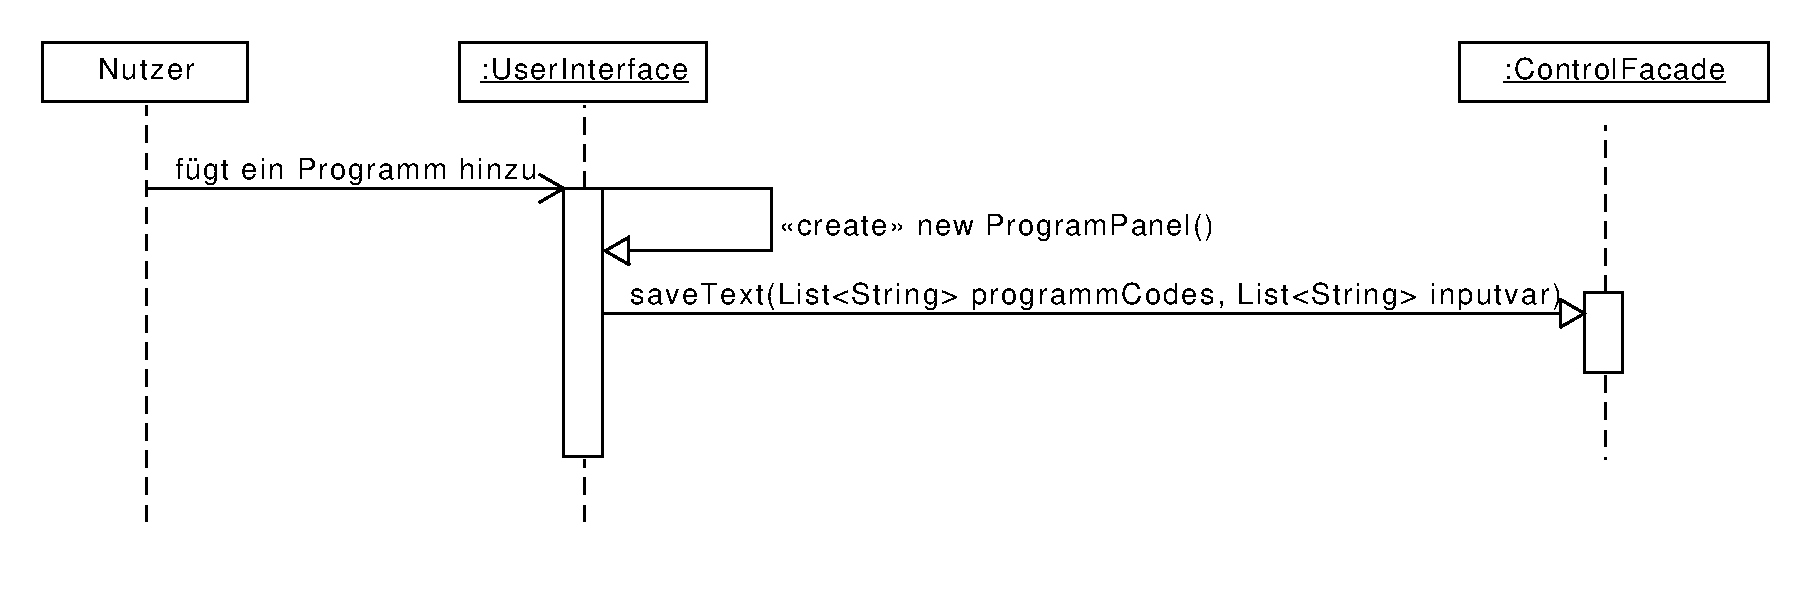
\includegraphics[width=1.0\textwidth]{diagrammIdeenUmlet/SequenceDiagrams/seq_AF10PDF.pdf}
\captionof{figure}{Sequenzdiagramm: Hinzufügen von Programmen durch den Menüeintrag}
\end{center}
Fügt der Benutzer über den Menüeintrag ein neues Programm hinzu, erstellt das UserInterface ein
neues ProgramPanel. Dies beschreibt die Funktionale Anforderung FA 170.
Fügt er ein neues Programm hinzu, indem er in ein bereits vorhandenes ProgramPanel seinen Programmcode kopiert (FA 160) oder schreibt (FA 150), gibt das UserInterface die Informationen an die Control weiter.
Diese Weitergabe von Informationen geschieht nach jedem Einfügen und Ändern von Programmtexten oder Eingabevariablen. Zum Start des Debugmodus gibt die Control alle diese Informationen an die DebugLogic weiter.

\newpage
\subsection{AF20: Ändern von Programmen}
\begin{center}
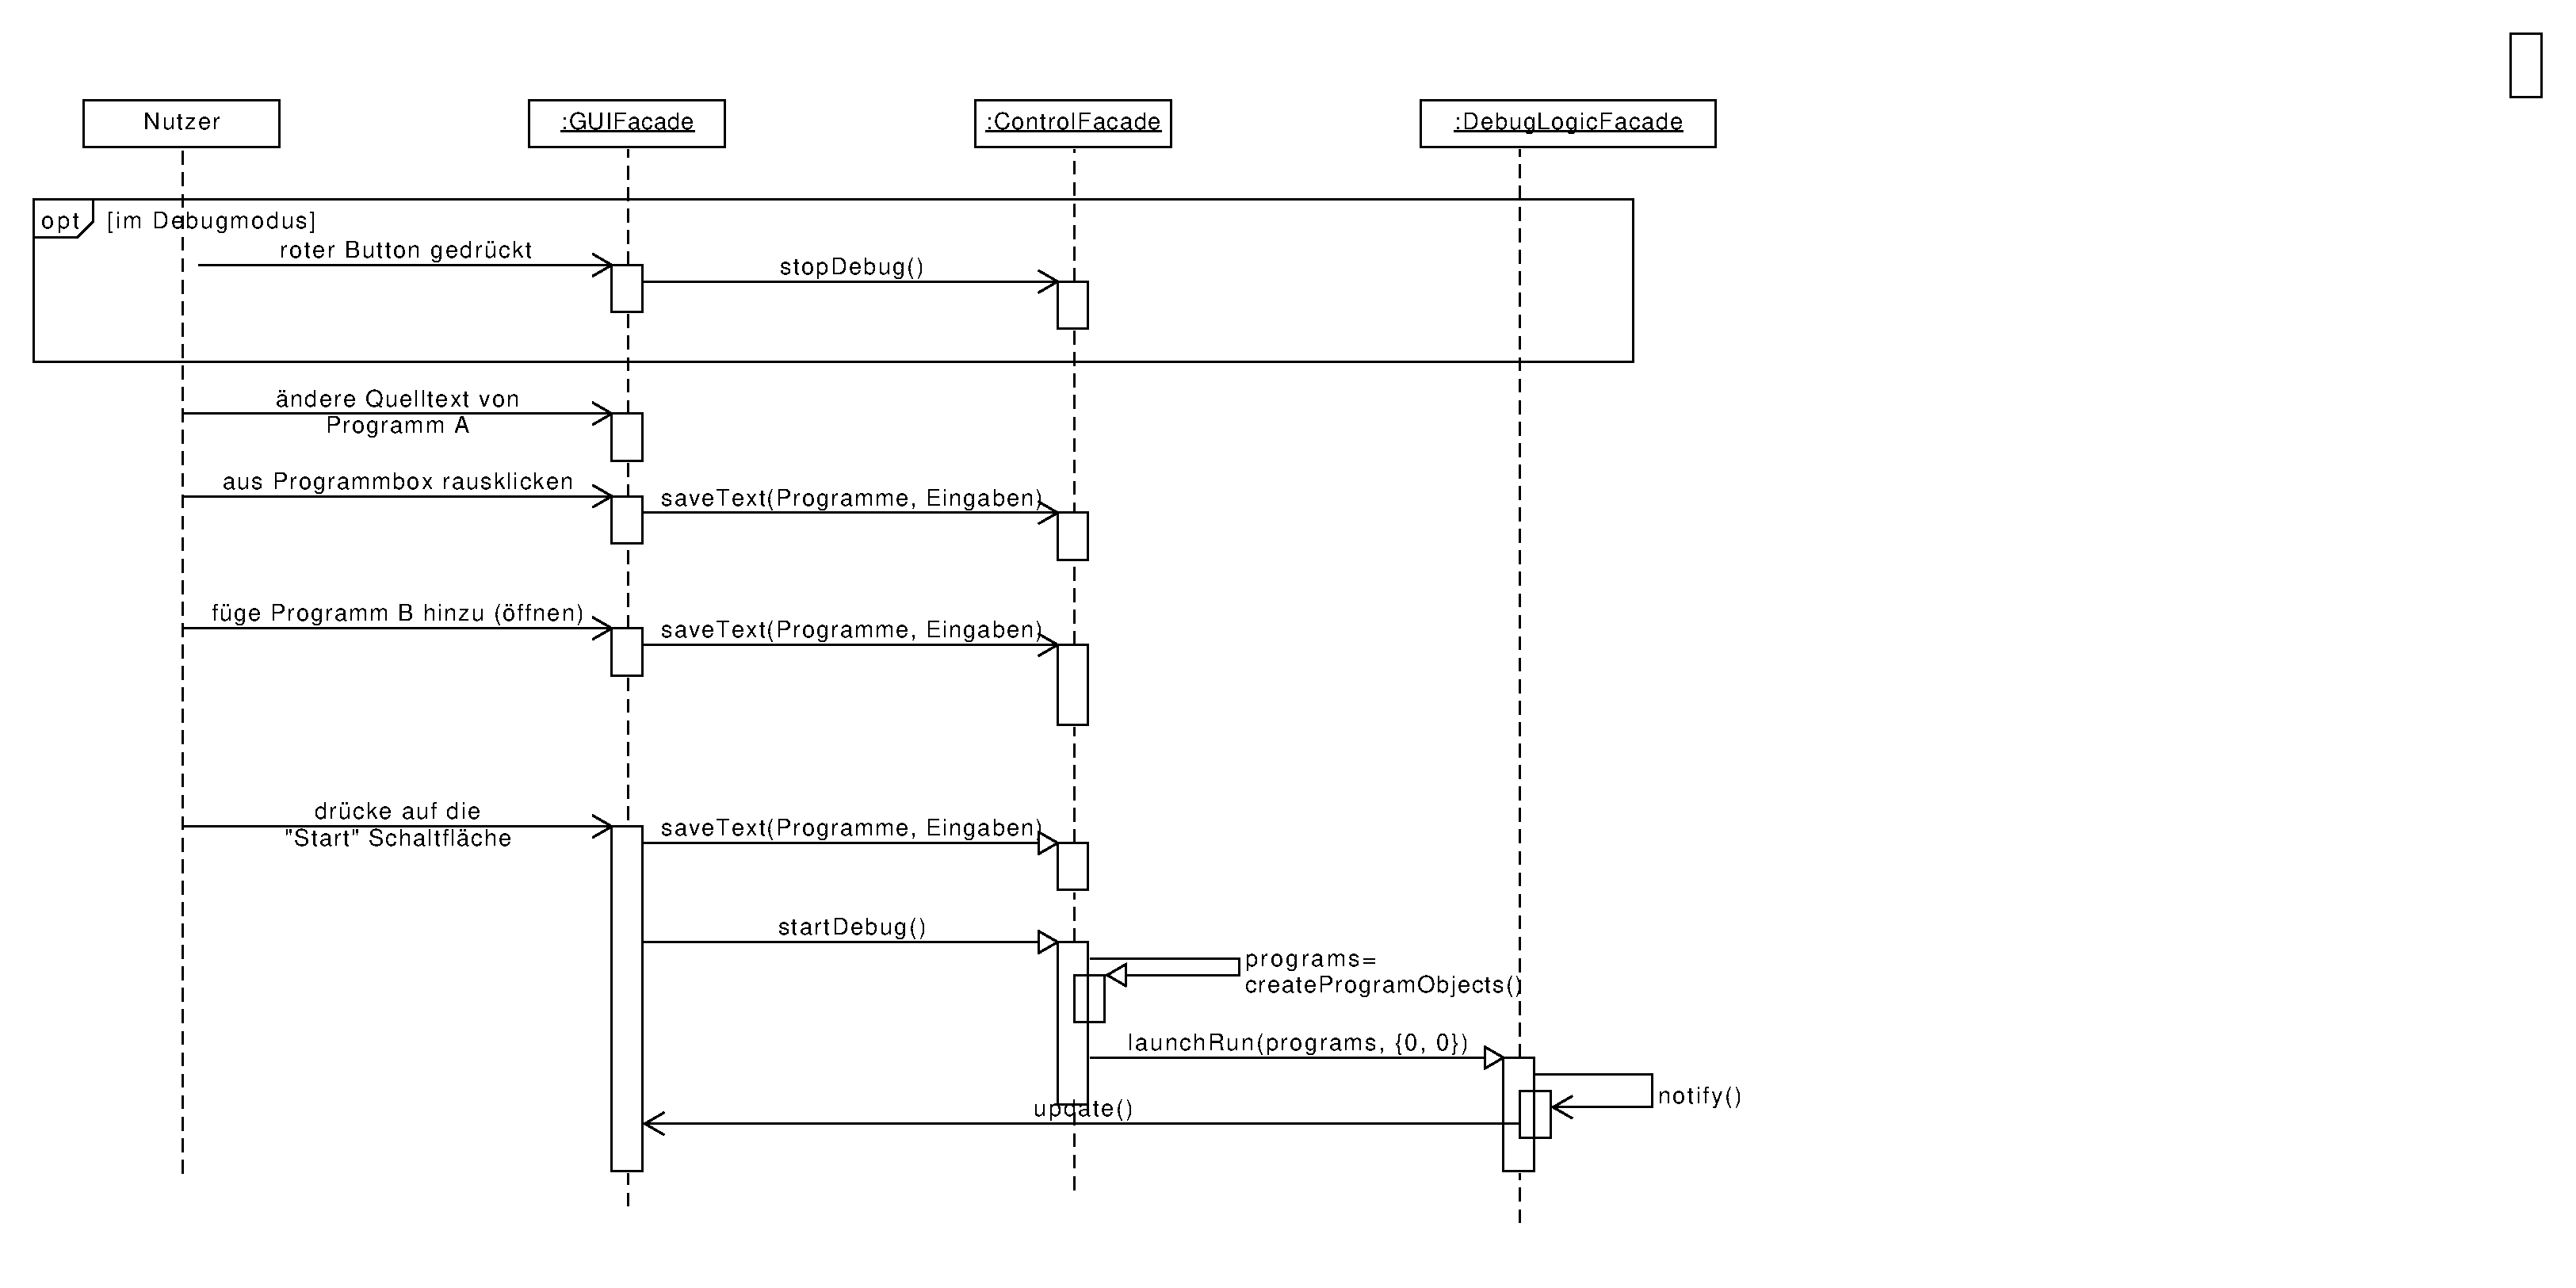
\includegraphics[width=1.0\textwidth]{diagrammIdeenUmlet/SequenceDiagrams/seq_AF20PDF.pdf}
\captionof{figure}{Sequenzdiagramm: Ändern von Programmen}
\end{center}
Möchte der Benutzer einen Programmtext editieren, muss er gegebenenfalls zunächst den Debugmodus beenden.
Anschließend lässt sich der Programmtext im Textfeld bearbeiten. Sobald der Benutzer außerhalb des
Textfelds klickt, gibt das MainInterface den neuen Programmtext und die Eingabeavariablen an die ControlFacade weiter. \\
Fügt der Benutzer einen neuen Programmtext durch Öffnen einer Datei hinzu, gibt das MainInterface diesen ebenfalls
mit den angegebenen Eingabevariablen an die ControlFacade weiter.\\
Sobald der Benutzer die Start-Schaltfläche auswählt um den Debugmodus zu starten, gibt das MainInterface erneut
alle eingegebenen Texte weiter und ruft schließlich startDebug() der ControlFacade auf. Diese erstellt aus den gespeicherten Informationen
Programm-Instanzen und gibt diese an die DebugLogicFacade weiter und startet damit den Debug-Lauf.

\newpage
\subsection{AF30: Setzen von Breakpoints}
\begin{center}
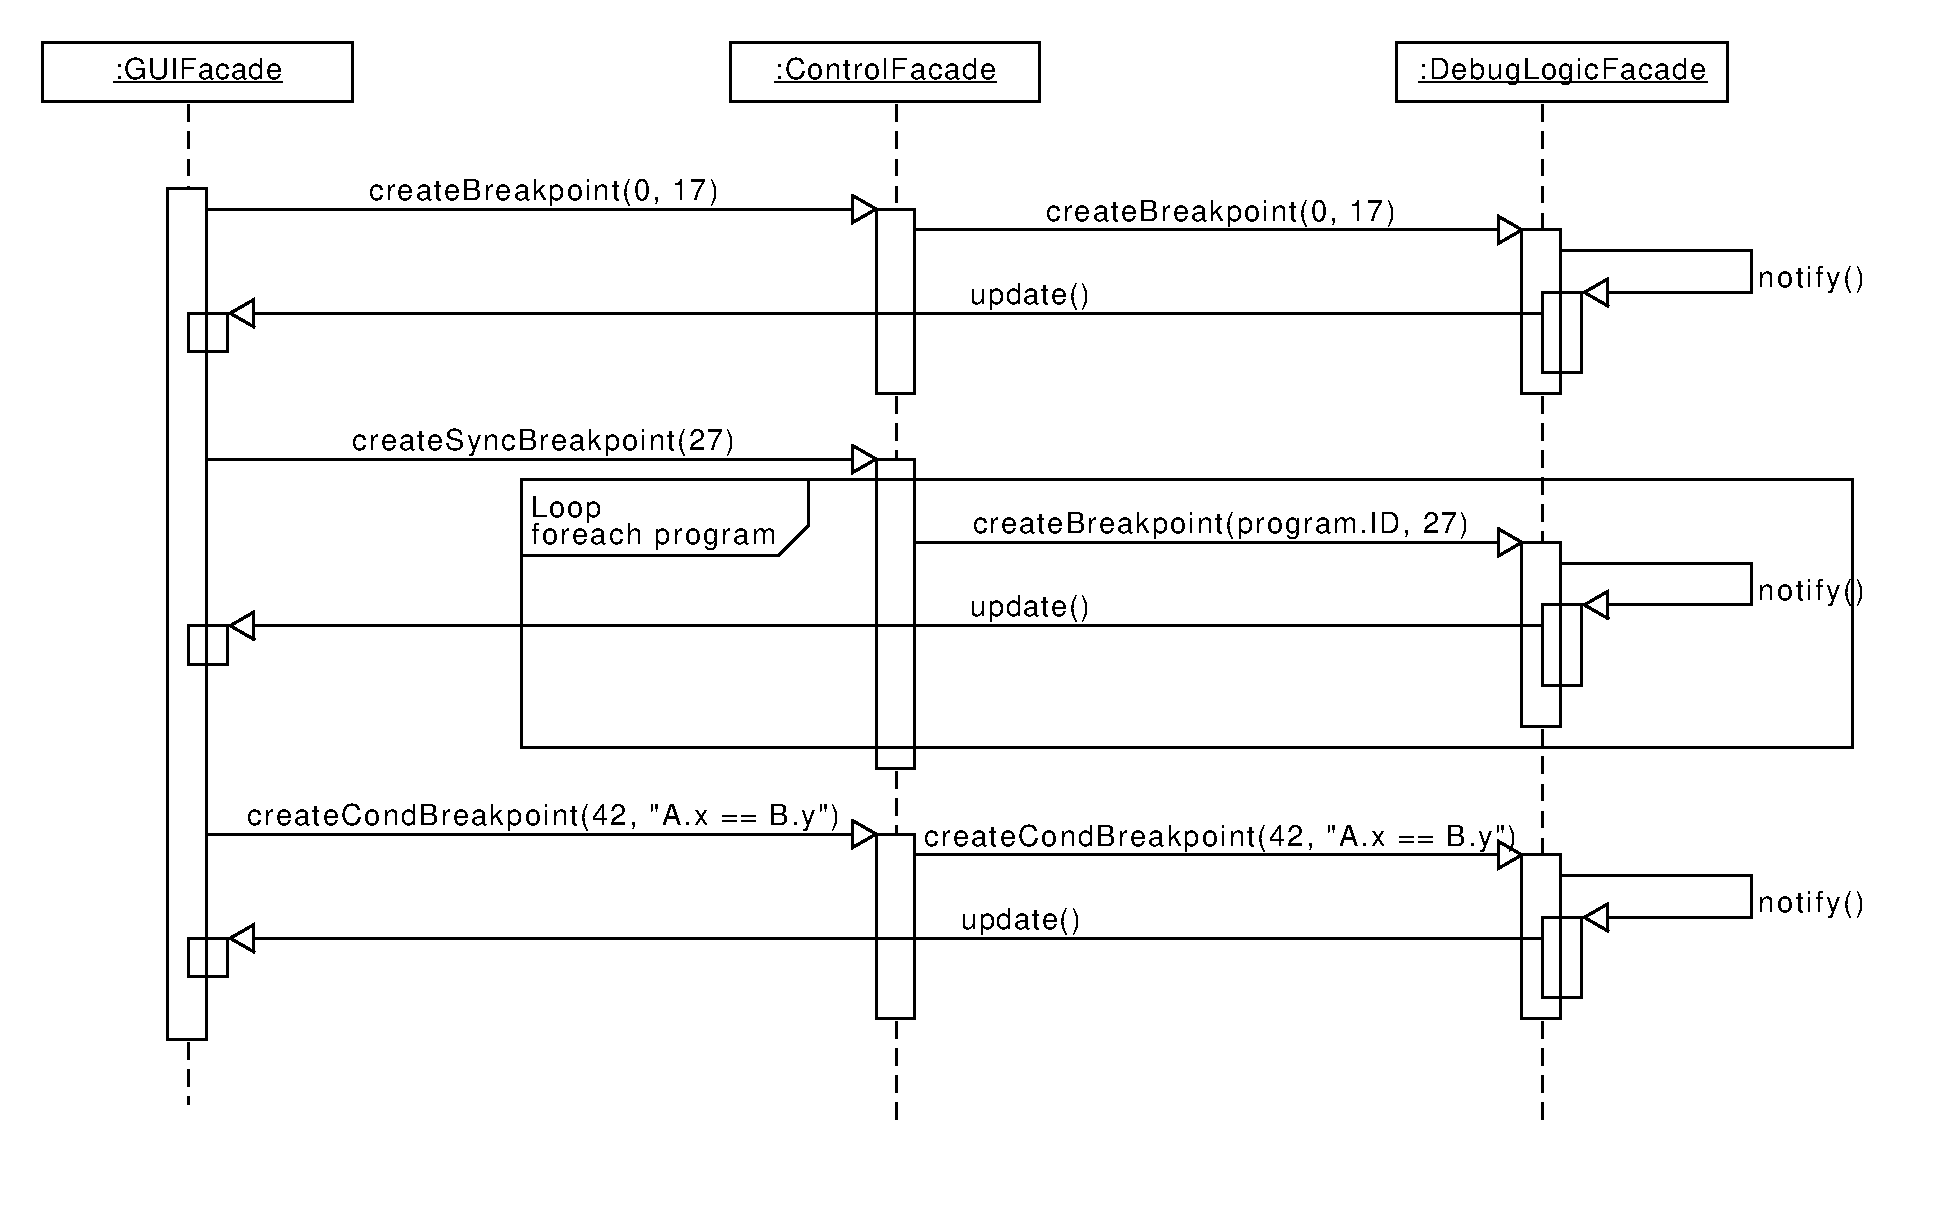
\includegraphics[width=1.0\textwidth]{diagrammIdeenUmlet/SequenceDiagrams/seq_breakpointsPDF.pdf}
\captionof{figure}{Sequenzdiagramm: Setzen von Breakpoints}
\end{center}
Setzt der Benutzer einen Breakpoint in eine Zeile in einem Programm, reicht das MainInterface
diese Information an die ControlFacade weiter, welche dann createBreakpoint mit der Programm-ID und der
Zeile an die DebugLogicFacade weitergibt.
Setzt der Benutzer jedoch einen Breakpoint in allen Programmen, teilt das
MainInterface dies der ControlFacade mit. Die ControlFacade ruft für jedes Programm
die Methode createBreakpoint der DebugLogicFacade auf.
Beim hinzufügen von bedingten Breakpoints gibt das MainInterface die ID des Breakpoints
und den vom Benutzer angegebenen Ausdruck an die ControlFacade weiter. Die Control reicht diese Informationen
ihrerseits an die DebugLogicFacade weiter, welche den Breakpoint ab diesem Zeitpunkt auswertet.

\newpage
\subsection{AF40: Hinzufügen von Watch-Expressions}
\begin{center}
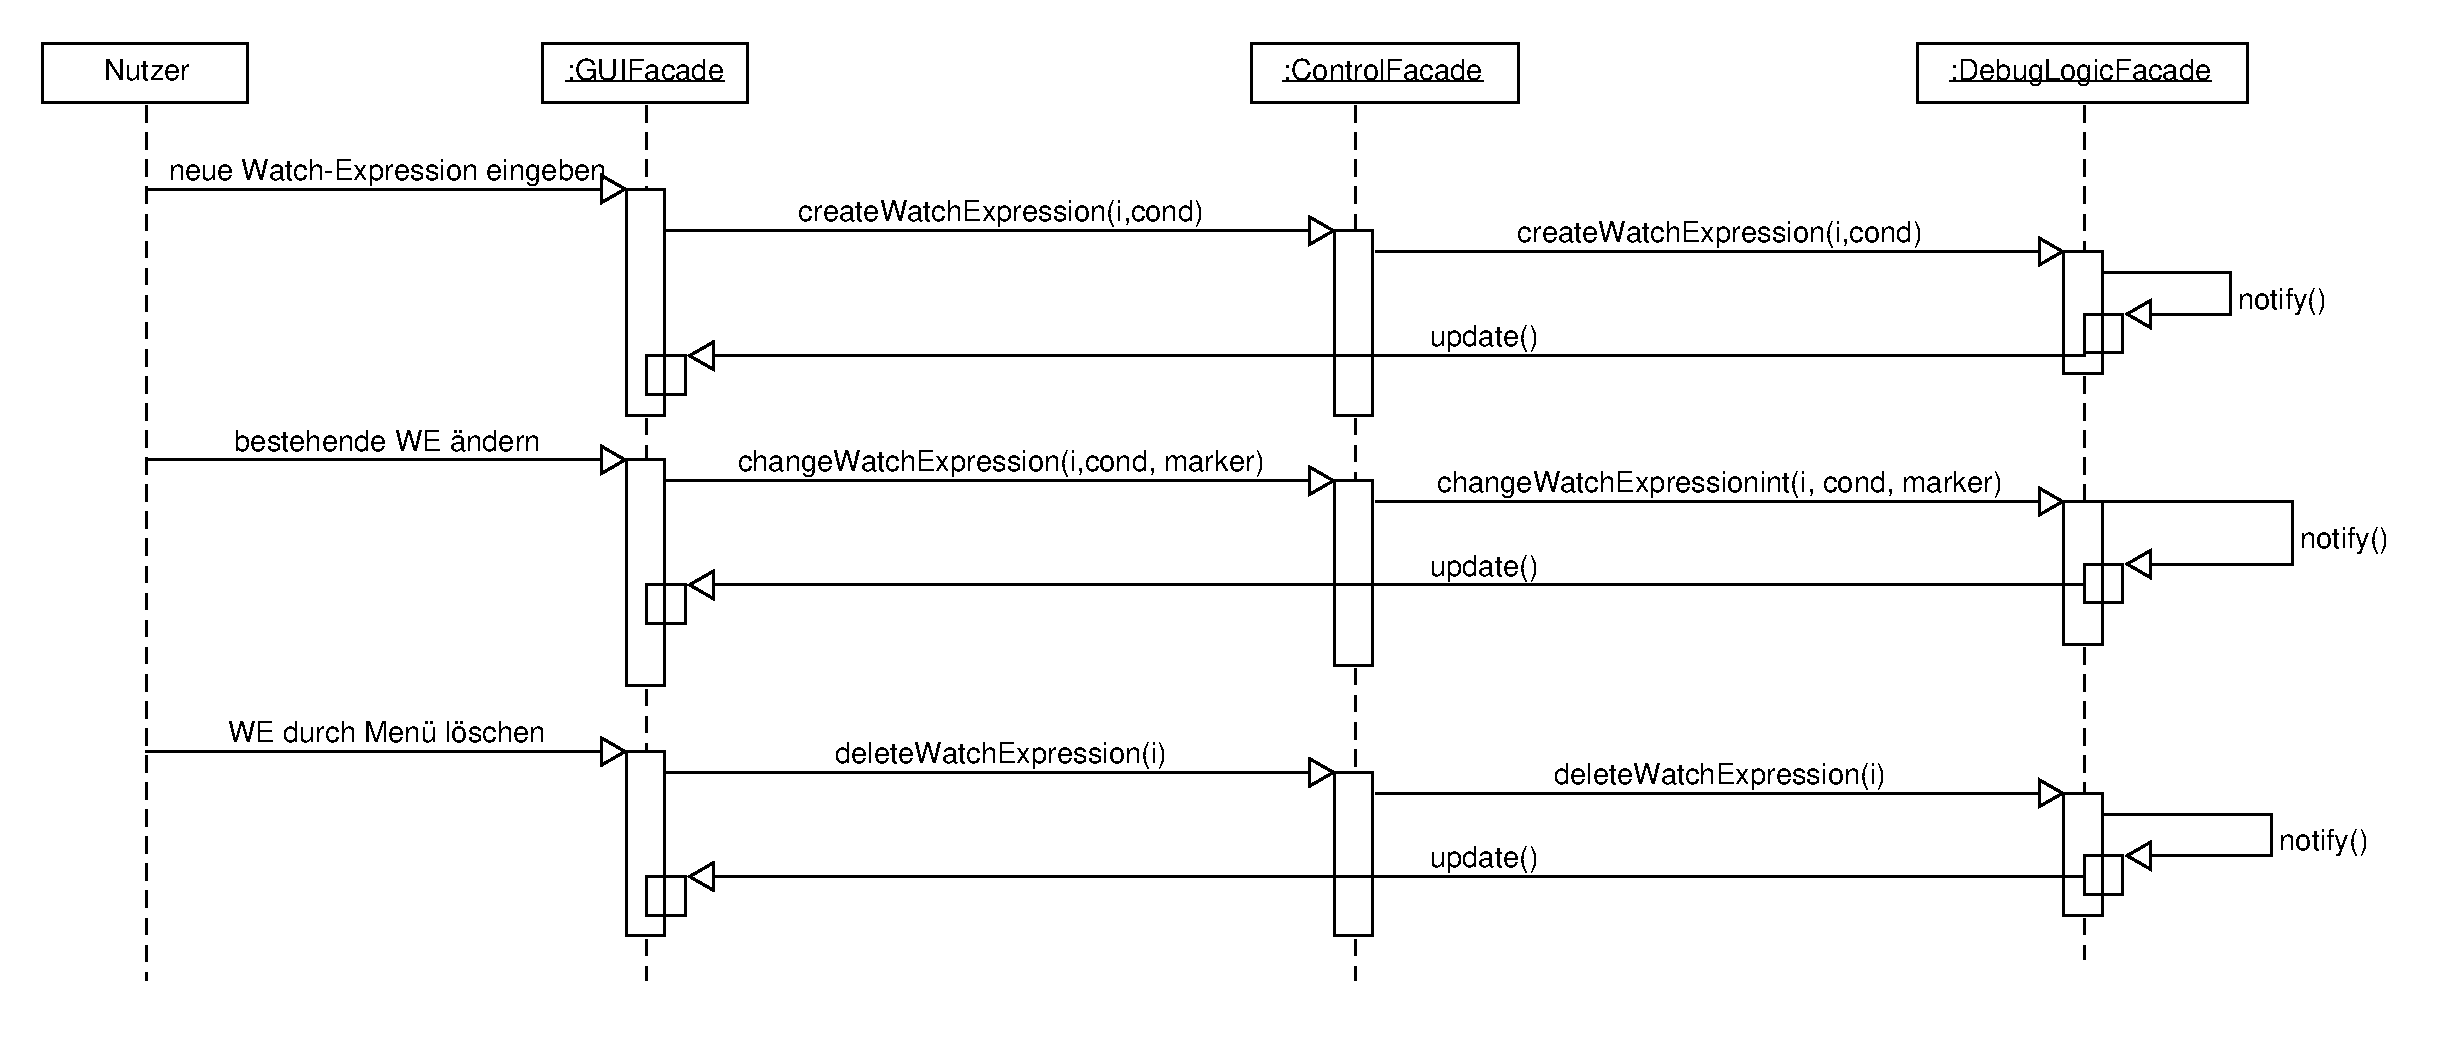
\includegraphics[width=1.0\textwidth]{diagrammIdeenUmlet/SequenceDiagrams/seq_WatchExpressionsPDF.pdf}
\captionof{figure}{Sequenzdiagramm: Hinzufügen von Watch-Expressions}
\end{center}
Die folgenden Vorgänge sind für Watch-Expressions (FA 110) und bedingte Breakpoints (FA 90) identisch. \\
Gibt der Benutzer eine neue Watch-Expression an, wird die Bedingung und die ID vom MainInterface über 
die Control an die DebugLogicFacade weitergegeben. Ändert der Benutzer die Watch-Expression, zB indem 
er die Bereichsbindung angibt (FA  120, bzw. FA 100 für bedingte Breakpoints), wird dies ebenfalls über die Control an die DebugLogicFacade weitergegeben.
Auch beim Löschen einer Watch-Expression über das entsprechende Menü der Benutzeroberfläche, erhält die
DebugLogic diese Information über die Control und stoppt das Auswerten dieser Watch-Expression.

\newpage
\subsection{Generieren von Vorschlägen}%TODO
\begin{center}
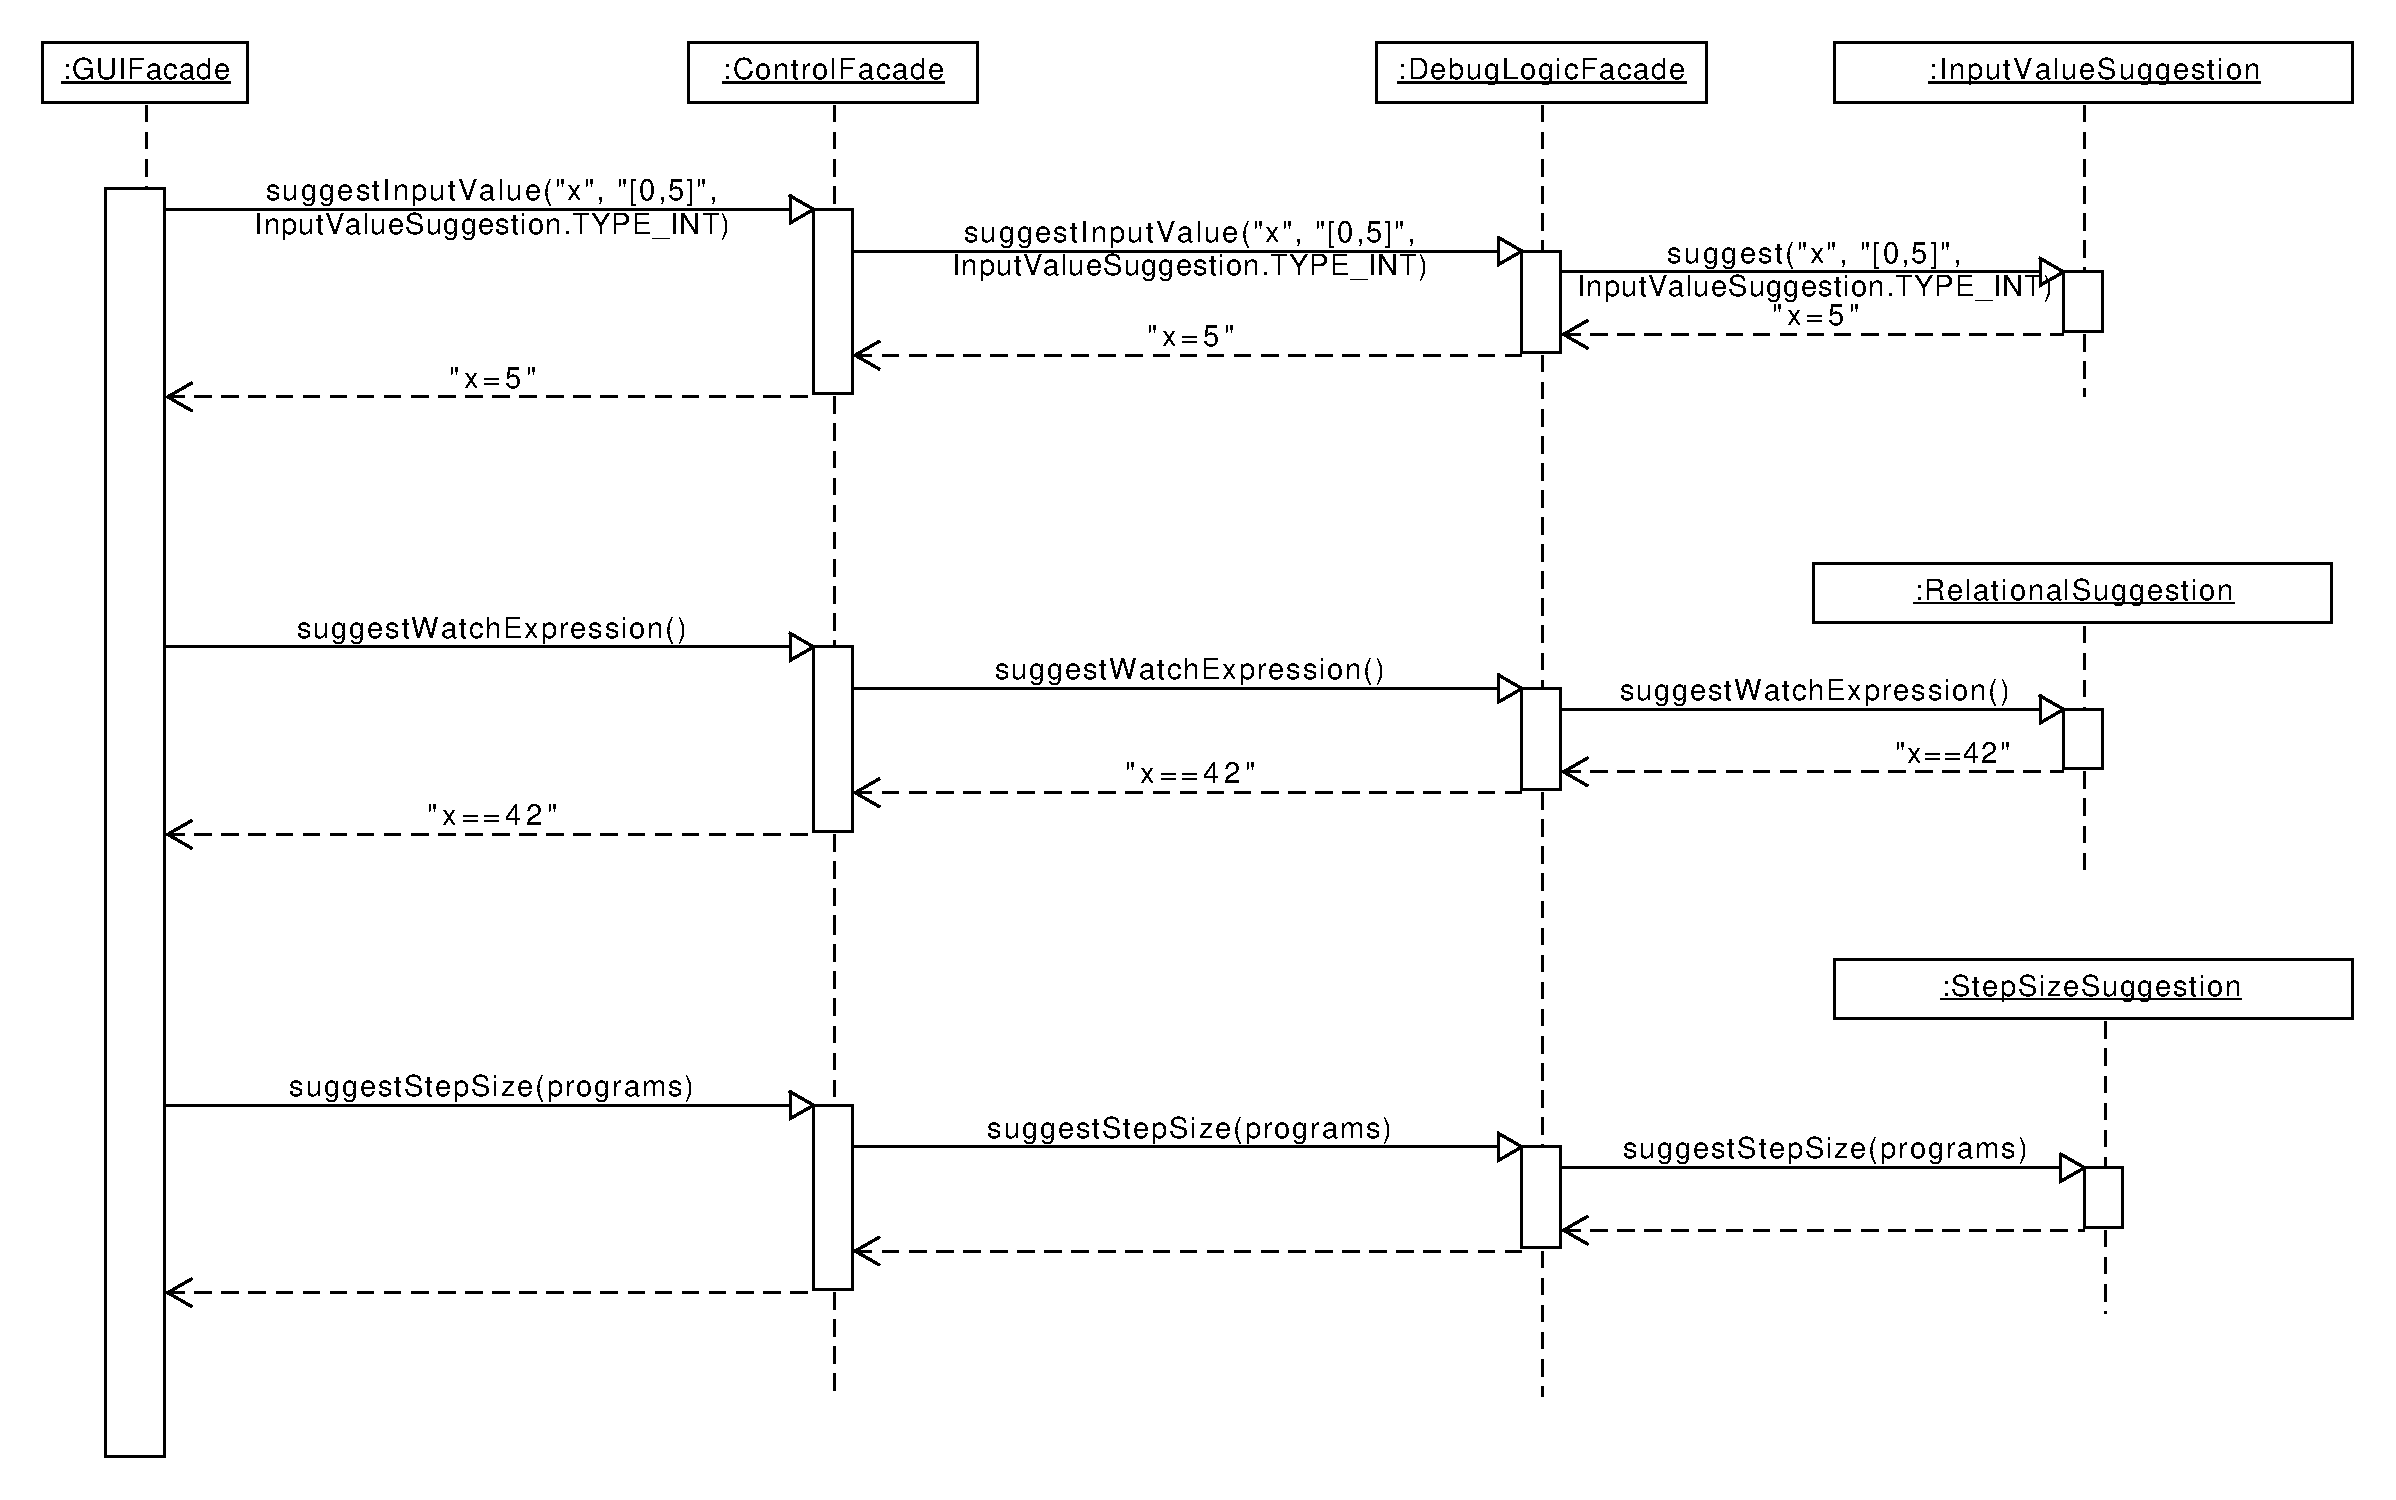
\includegraphics[width=1.0\textwidth]{diagrammIdeenUmlet/SequenceDiagrams/seq_suggestions.pdf}
\captionof{figure}{Sequenzdiagramm: Generierung von Vorschlägen für Watch-Expressions, bedingte Breakpoints, Schrittgrößen und Eingaben}
\end{center}
Möchte der Benutzer sich eine Watch-Expression vorschlagen lassen (FA 270), so wird nach Anklicken des dazugehörigen Buttons der Befehl über die ControlFacade zur DebugLogicControl weitergeleiten. Dort wird dieser an eine Vorschlagsstrategie (z.B. EquivalenceSuggestionStrategy) gesendet und dort verarbeitet. Nachdem ein Vorschlag generiert wurde wird dieser als Zeichenkette, welche die finale Watch-Expression Bedingung repräsentiert, an die GUIFacade zurückgegeben. Danach fügt die GUI wie in AF40 eine Watch-Expression mit der erhaltenen Bedingung hinzu.
\\
Bedingte Breakpoints lassen sich auf die gleiche Weise generieren (FA 280).
\\
Schrittgrößen werden ähnlich vorgeschlagen (FA 300), hierbei werden der Control die Programme übergeben, welche diese an die DebugLogic weitergibt. Dies ist nötig, damit die Schrittgröße anhand der Programmcodes errechnet werden kann.
\\
Eingaben können ebenfalls ähnlich vorgeschlagen werden (FA 220), jedoch muss der Nutzer hier angeben, für welche Variable, für welchen Variablentyp und in welchem Intervall er einen Vorschlag erhalten möchte.

\newpage
\subsection{AF50: Programme debuggen}
\begin{center}
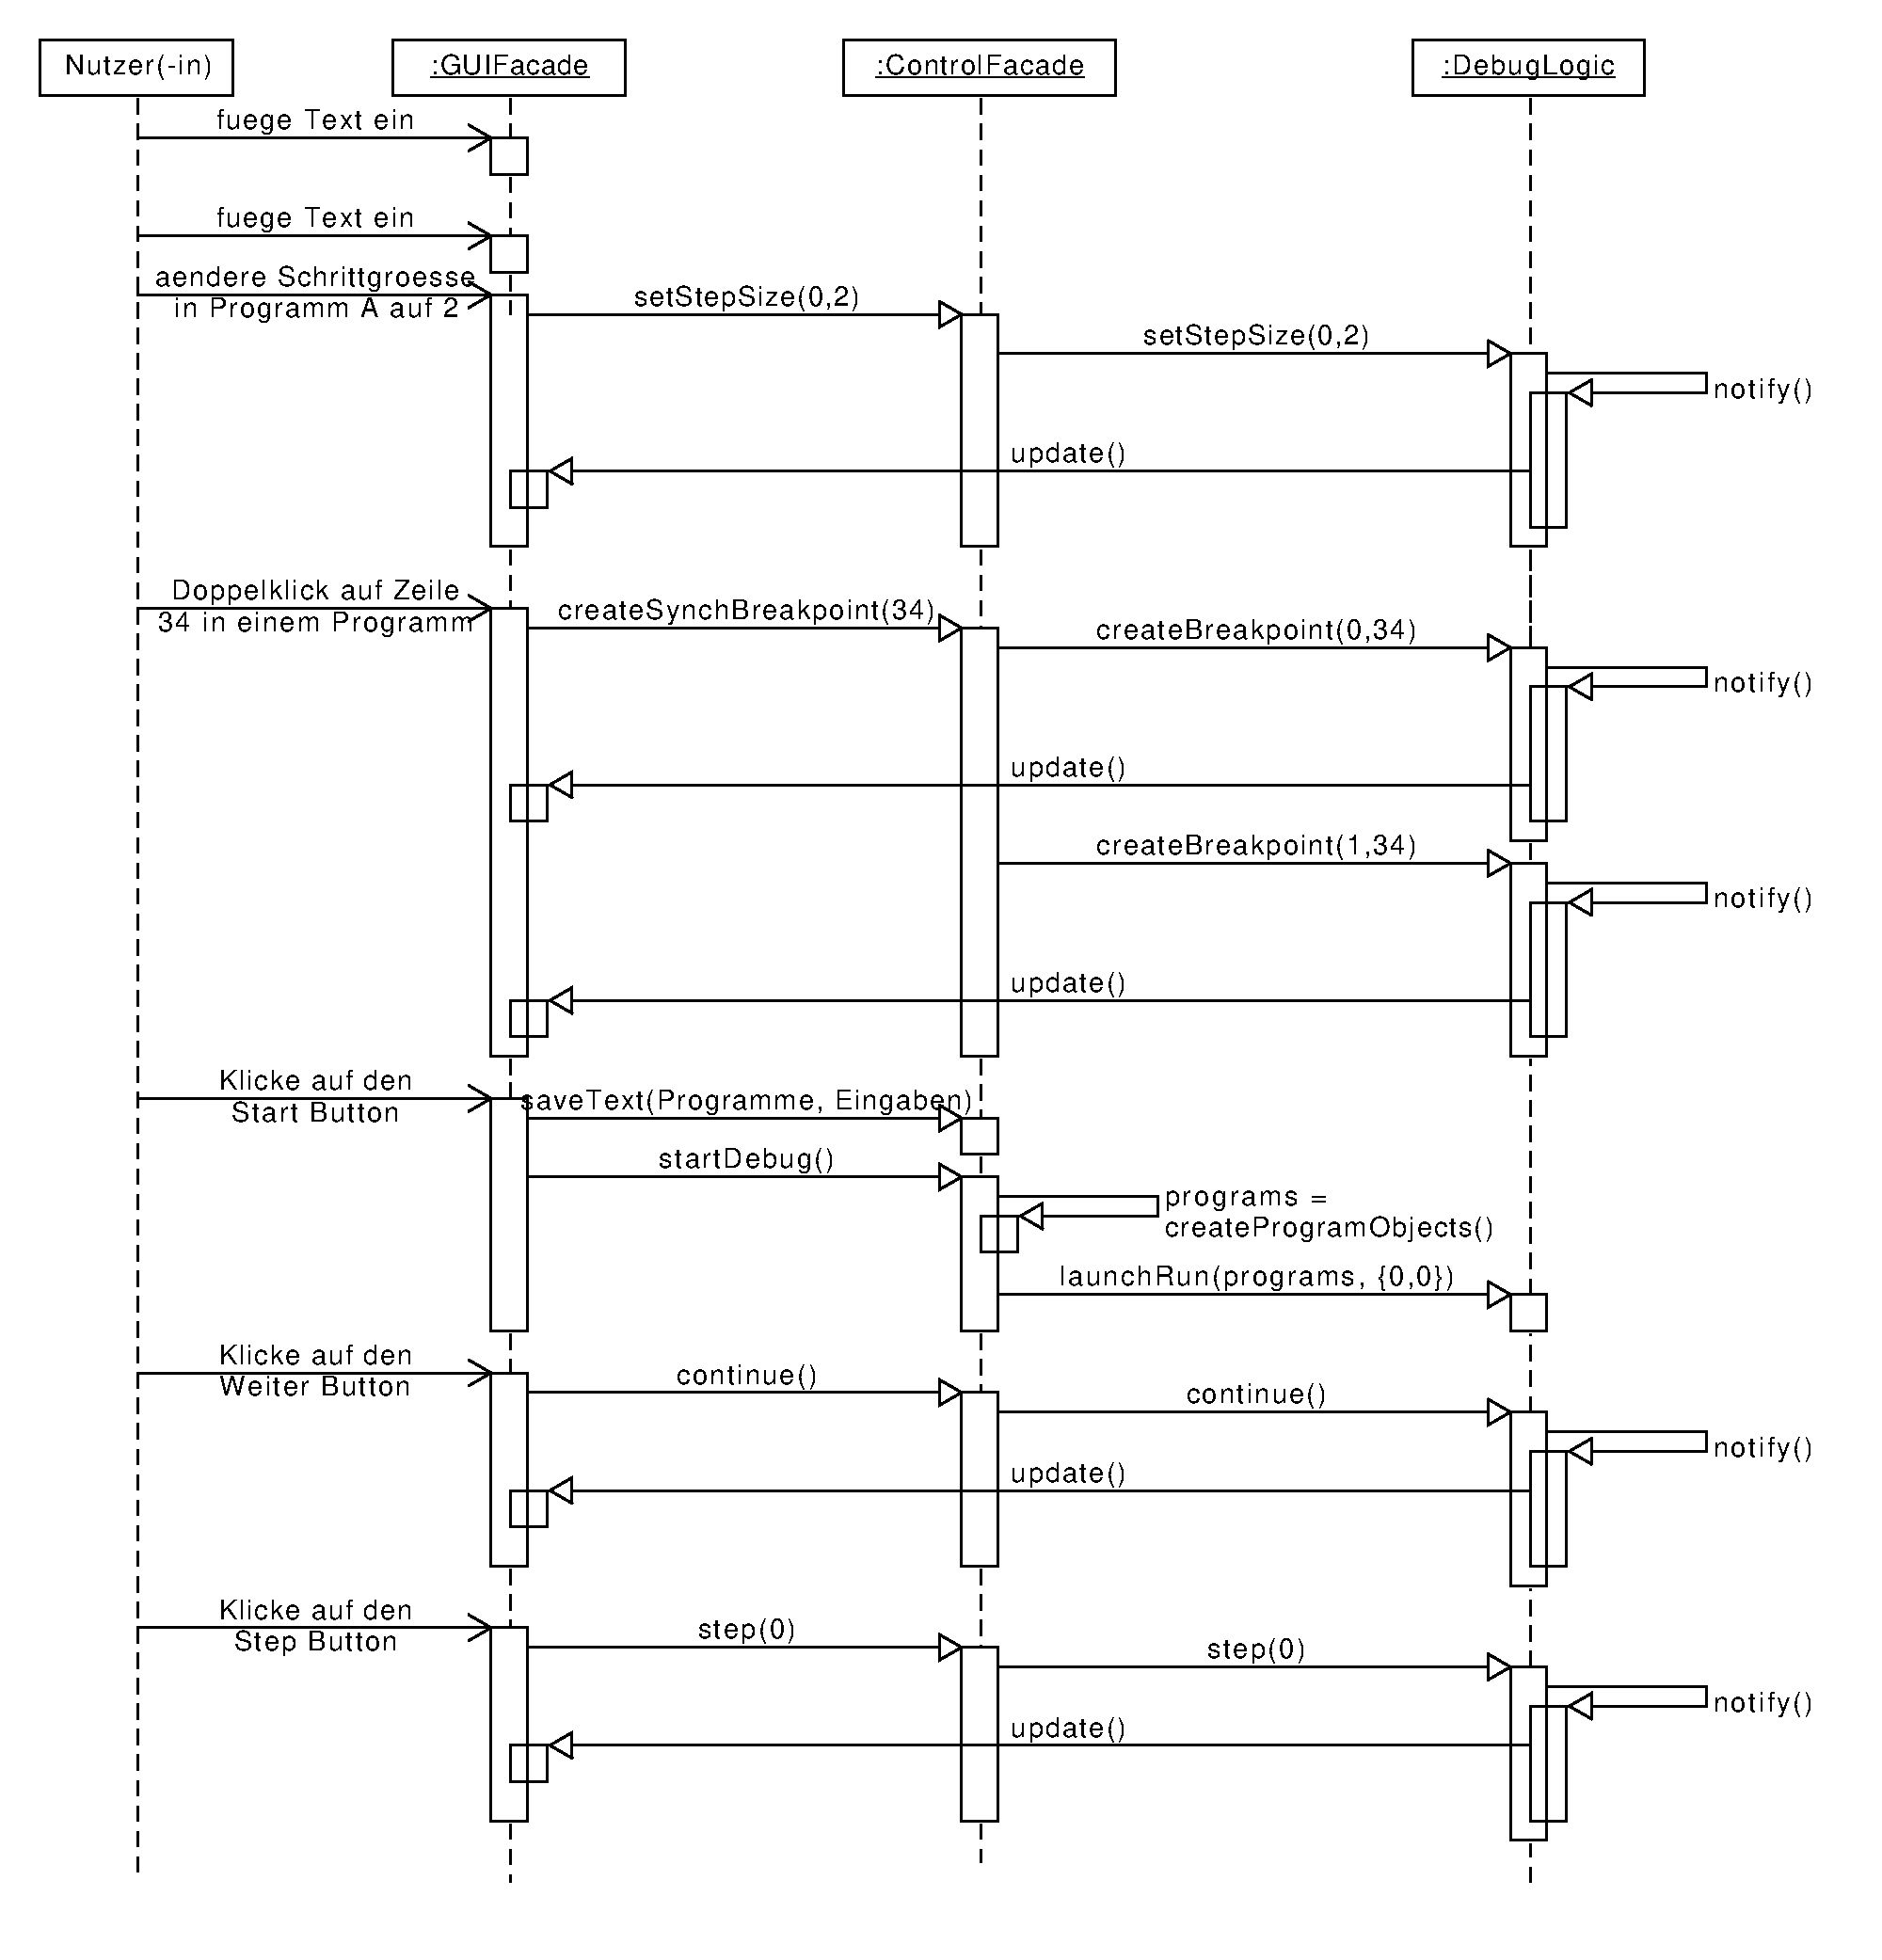
\includegraphics[width=0.9\textwidth]{diagrammIdeenUmlet/SequenceDiagrams/seq_AF50PDF.pdf}
\captionof{figure}{Sequenzdiagramm: Debuggen von Programmen}
\end{center}
Dieses Sequenzdiagramm fasst die Schritte des Nutzers bei einem Debug-Lauf zusammen (FA 10).
Hierbei werden vor Start des DIbuggers Programme hinzugefügt, die Schrittgröße geändert und Breakpoints hinzugefügt.
Sobald der Benutzer auf Start klickt, werden seine Eingaben final gespeichert und die Control startet 
den DebugLauf der DebugLogic.
Wenn der Benutzer durch Weiter (FA 130), Schritt (FA 20)oder Einzelschritt (FA 30) durch den DebugLauf navigiert, werden diese Befehle über
die Control an die DebugLogic weitergegeben. Die Schritte werden von der DebugLogic ausgeführt, und anschließend
wird die GUIFacade als Beobachter dazu aufgefordert, die aktualisierten Werte anzuzeigen.
\subsection{Erzeugung abstrakter Strukturen im Subpaket Interpreter}
In diesem Abschnitt soll die Funktionalität des Subpaketes \textit{DebugLogic.Interpreter} beschrieben werden. Der Interpreter hat im Wesentlichen zwei Aufgaben: Einerseits muss er für WatchExpressions und bedingte Breakpoints eine abstrakte Struktur aufbauen, die sich einfach auswerten lässt. Andererseits hat er die Aufgabe, den kompletten Programmverlauf(im Folgenden \enquote{Trace})  eines Programmes zu berechnen und einen Iterator darüber bereitzustellen.
\subsubsection{Erzeugung einer abstrakten Repräsentation für Watch-Expressions und bedingte Breakpoints}
Watch-Expressions und bedingte Breakpoints bestehen immer aus einem vom Nutzer spezifizierten Ausdruck über den Variablen der vorkommenden Programme. Syntaktisch handelt es sich bei diesem Ausdruck einfach um einen Term. Semantisch muss aber bei bedingten Breakpoints sichergestellt sein, dass es sich um einen Term handelt, der sich zu einem Wahrheitswert auswertet. 
%Wie Terme in der Klassenstruktur aufgebaut sind, ist im Kapitel \ref{Patterns} %genauer beschrieben. 
Zusätzlich enthalten Watch-Expressions und bedingte Breakpoints einen Gültigkeitsbereich in Form von mehreren \textit{ScopeTuple}-Instanzen. 
\\
In den hier abgebildeten Diagrammen sind der Übersichtlichkeit halber nur die für die Erklärung wichtigsten Klassen meist ohne Methoden oder Attribute zu sehen.
Wir betrachten das Diagramm \ref{WEBBP}.  
\begin{center}
\makebox[\textwidth][c]{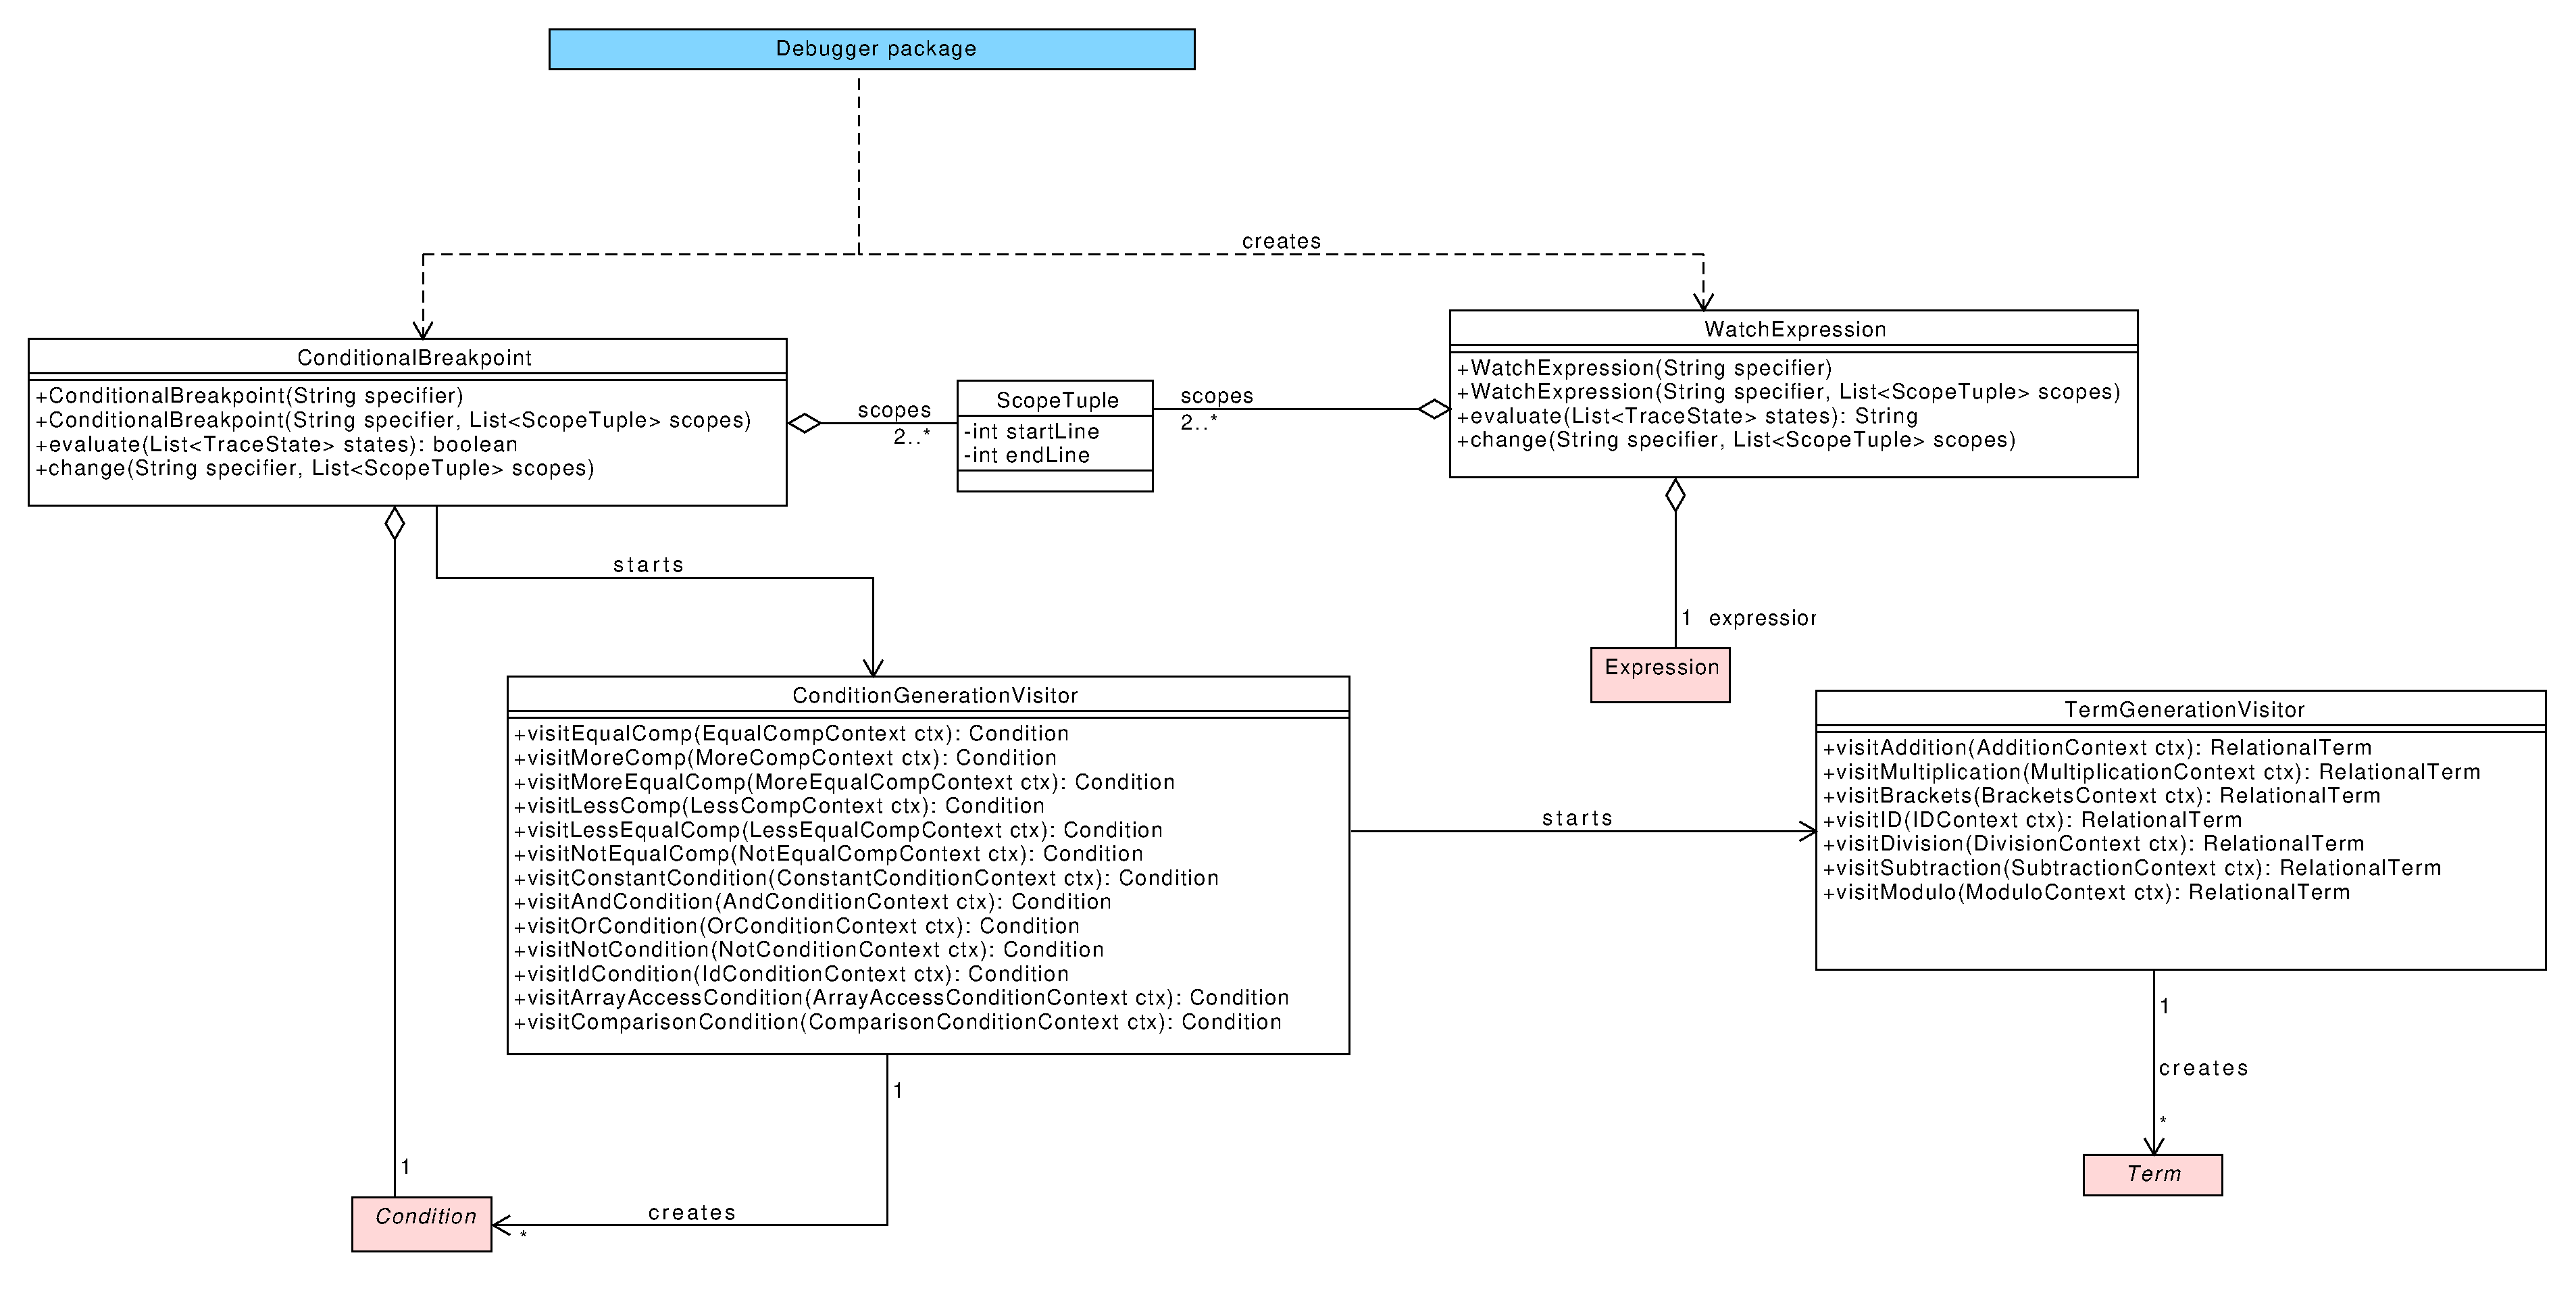
\includegraphics[width=1.45\textwidth]{diagrammIdeenUmlet/WatchExpressions.pdf}}
\captionof{figure}{Watch-Expressions und Bedingte Breakpoints}
\label{WEBBP}
\end{center}
Das Debuggerpaket erzeugt einen neuen Bedingten Breakpoint und übergibt dazu eine Zeichenkette, die diesen spezifiziert. Der Bedingte Breakpoint nutzt das Paket \textit{AntlrParser}, um einen Syntaxbaum zu erzeugen. Dann wird ein \textit{TermGenerationVisitor} gestartet, der diesen Syntaxbaum abläuft und dabei eine \textit{Condition} erzeugt. Beim Erzeugen einer WatchExpression passiert das gleiche. Die Gültigkeitsbereiche können entweder bei Erzeugung direkt mitübergeben werden oder erst später durch Aufruf der \textit{change()}-Methode hinzugefügt werden. Standardmäßig ist der Gültigkeitsbereich maximal.
\newpage

\begin{landscape}
\subsubsection{Erzeugung des Traces}
\begin{center}
\makebox[\textwidth][c]{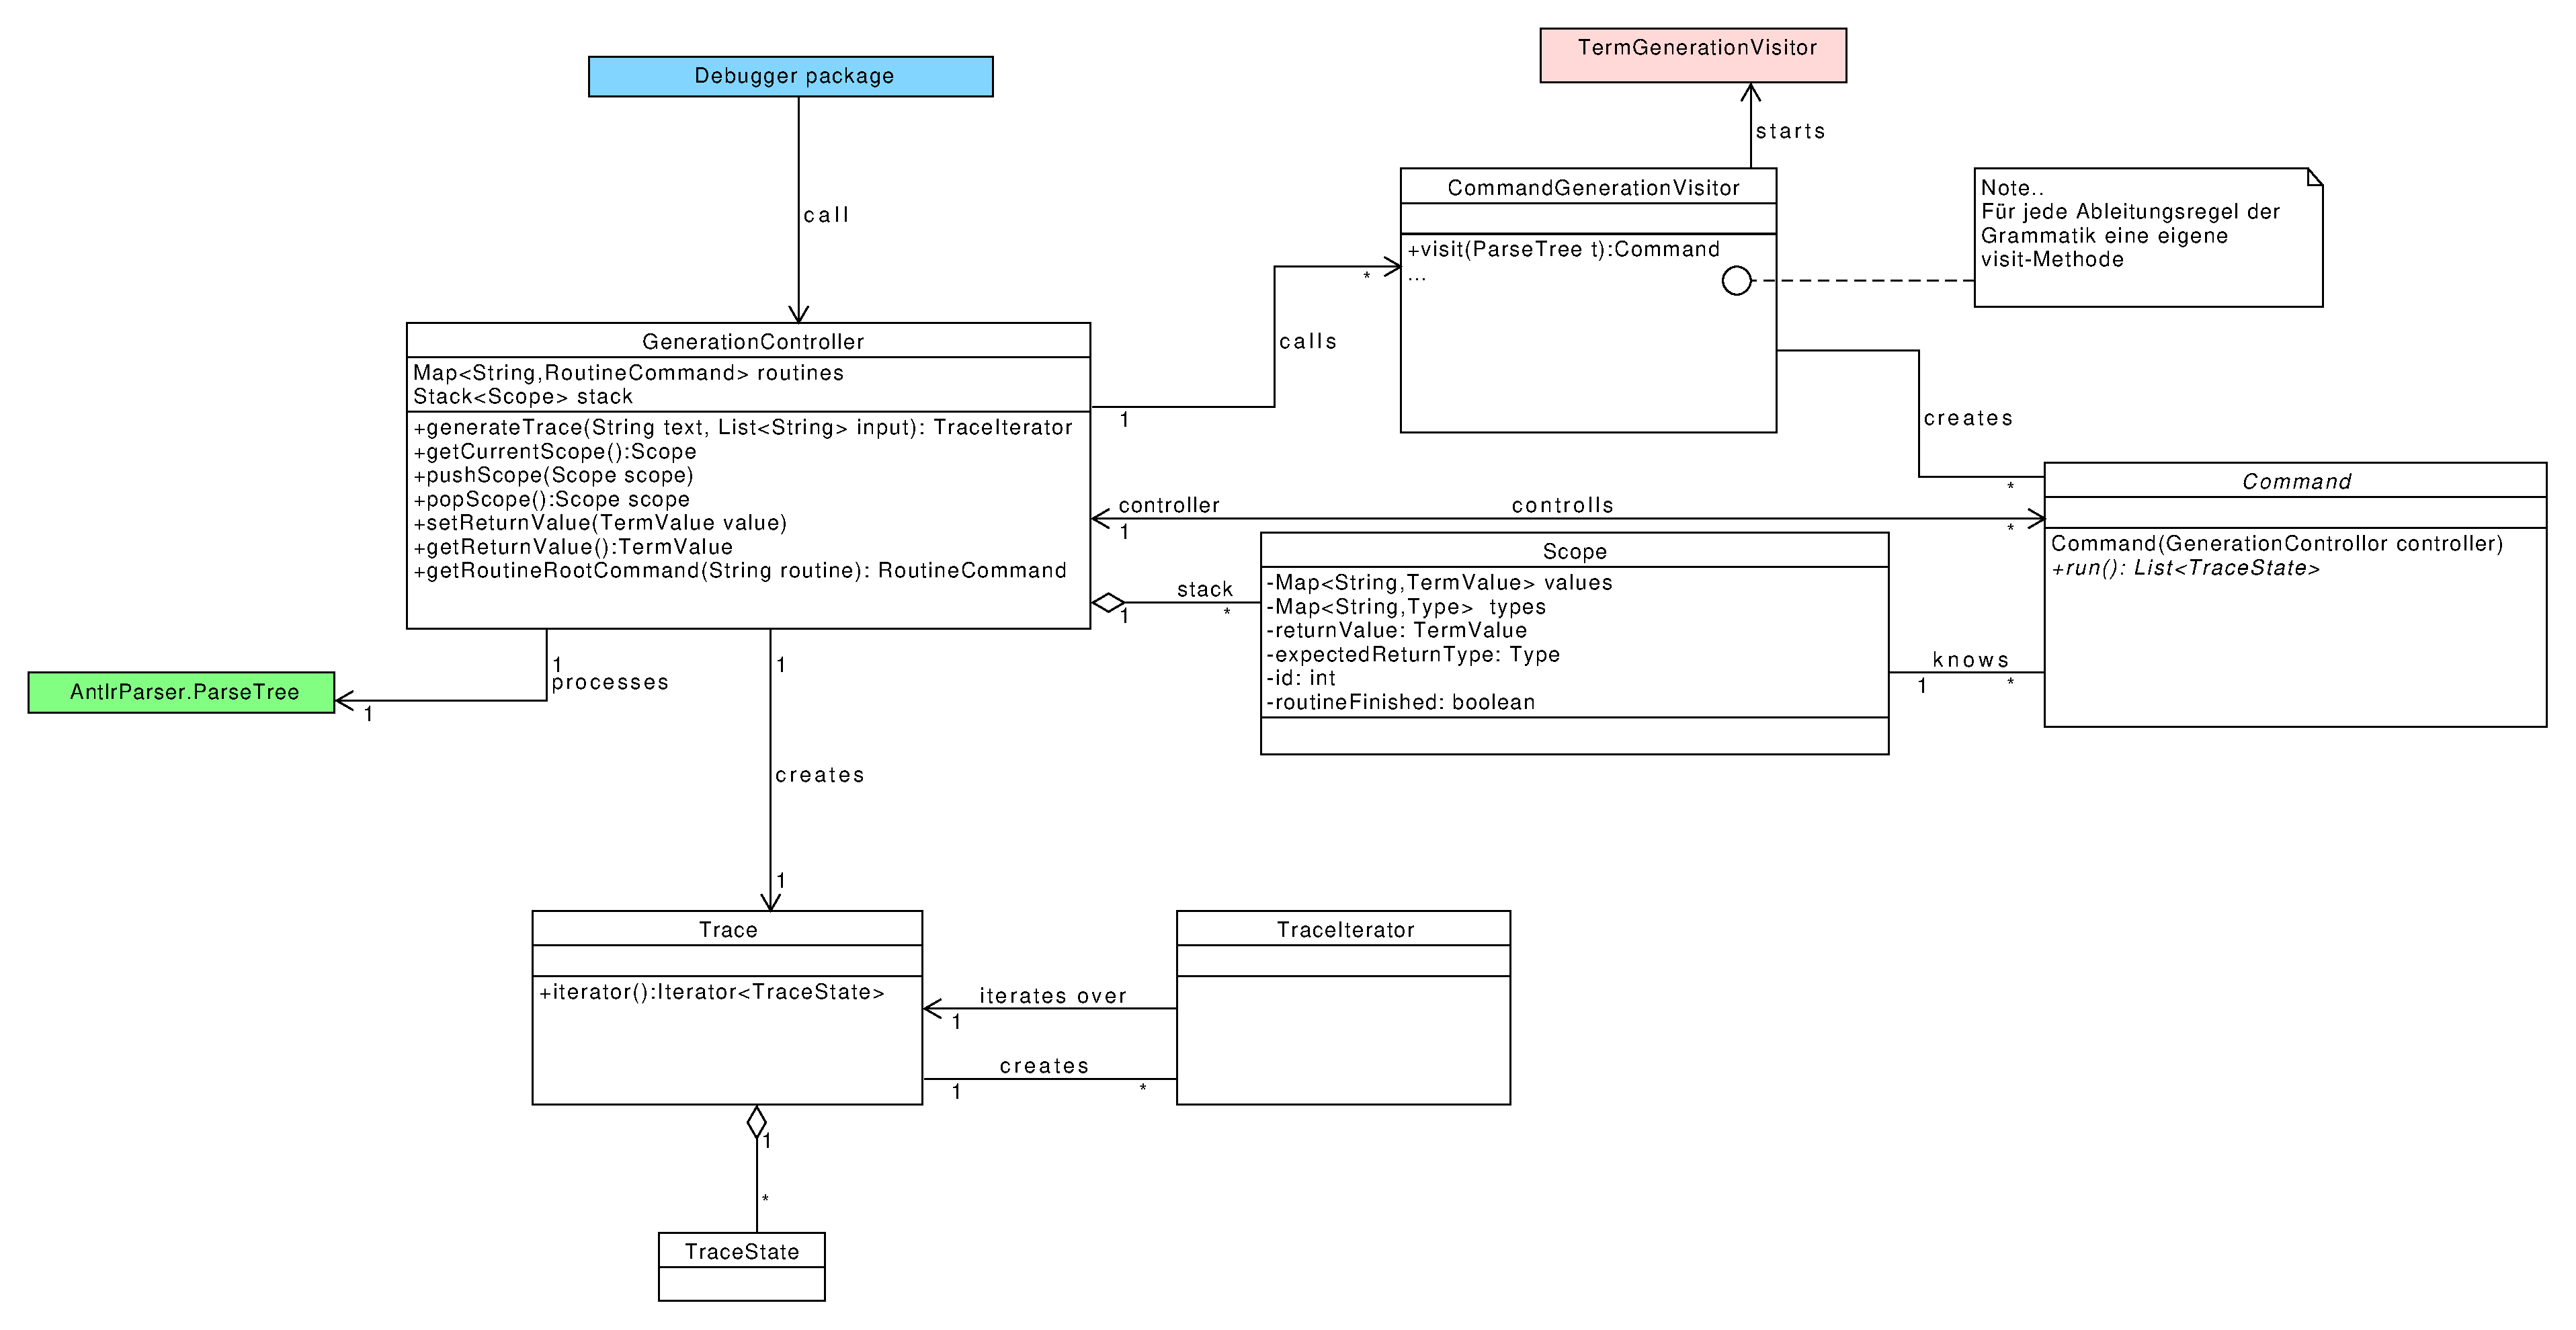
\includegraphics[width=1.6\textwidth]{diagrammIdeenUmlet/TraceGenerationClasses.pdf}}
\captionof{figure}{An der Tracegenerierung beteiligte Klassen}
\label{TraceGen}
\end{center}
\end{landscape}
\newpage
Gegeben sei das folgende (Wlang-)Programm:
\begin{verbatim}
int foo() {
    return 1+2+3;
}
int main(){
    int x;
    int y=3;
    while(x<(y+7)%4){
        x=x+1;
    }
    return c;
}
\end{verbatim}

Die Zusammenarbeit der in Abbildung \ref{TraceGen} gegebenen Klassen soll nun an diesem Beispiel erklärt werden. 
Die Klasse \textit{GenerationController} steuert das Verfahren der Traceerzeugung. Sie bekommt in der Methode \textit{generateTrace()} den Quelltext und die Eingaben für diesen übergeben. Zunächst wird vom Subpaket \textit{DebugLogic.AntlrParser} ein \textit{ParseTree} erzeugt. Für obiges Beispielprogramm ist dieser in Abbildung \ref{ParseTreeExample} zu sehen.
\begin{center}
\makebox[\textwidth][c]{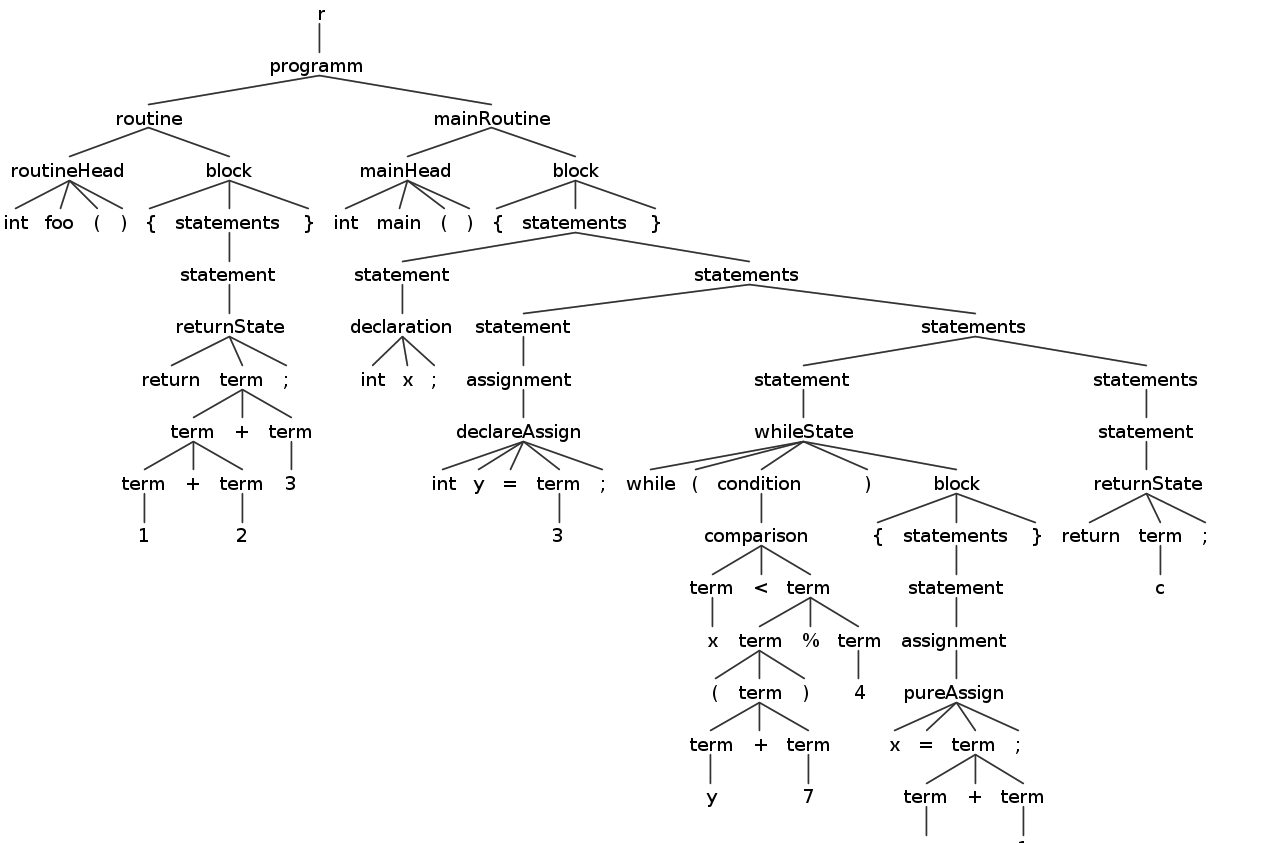
\includegraphics[width=1.0\textwidth]{diagrammIdeenUmlet/parseTreeExample.png}}
\captionof{figure}{Beispiel für einen Ableitungsbaum}
\label{ParseTreeExample}
\end{center}
Über diesen Baum läuft der \textit{CommandGenerationVisitor} und erzeugt für jede Routine einen Baum aus Befehlen (\textit{Command}-Kompositum). Dabei verwendet er einen weiteren Visitor, die Terme in Form der in Kapitel \ref{Terme} gegebenen Klassen erzeugen. 
Die Wurzeln dieser Bäume aus Befehlen werden im \textit{GenerationController} in der Map \textit{routines} gespeichert, sodass sie dann über ihren Routinennamen aufrufbar sind. Die Objektstruktur nach diesem Schritt sieht dann wie im Objektdiagramm (Abbildung \ref{CommandTreeExample}) aus.
\begin{figure}[!h]
\makebox[\textwidth][c]{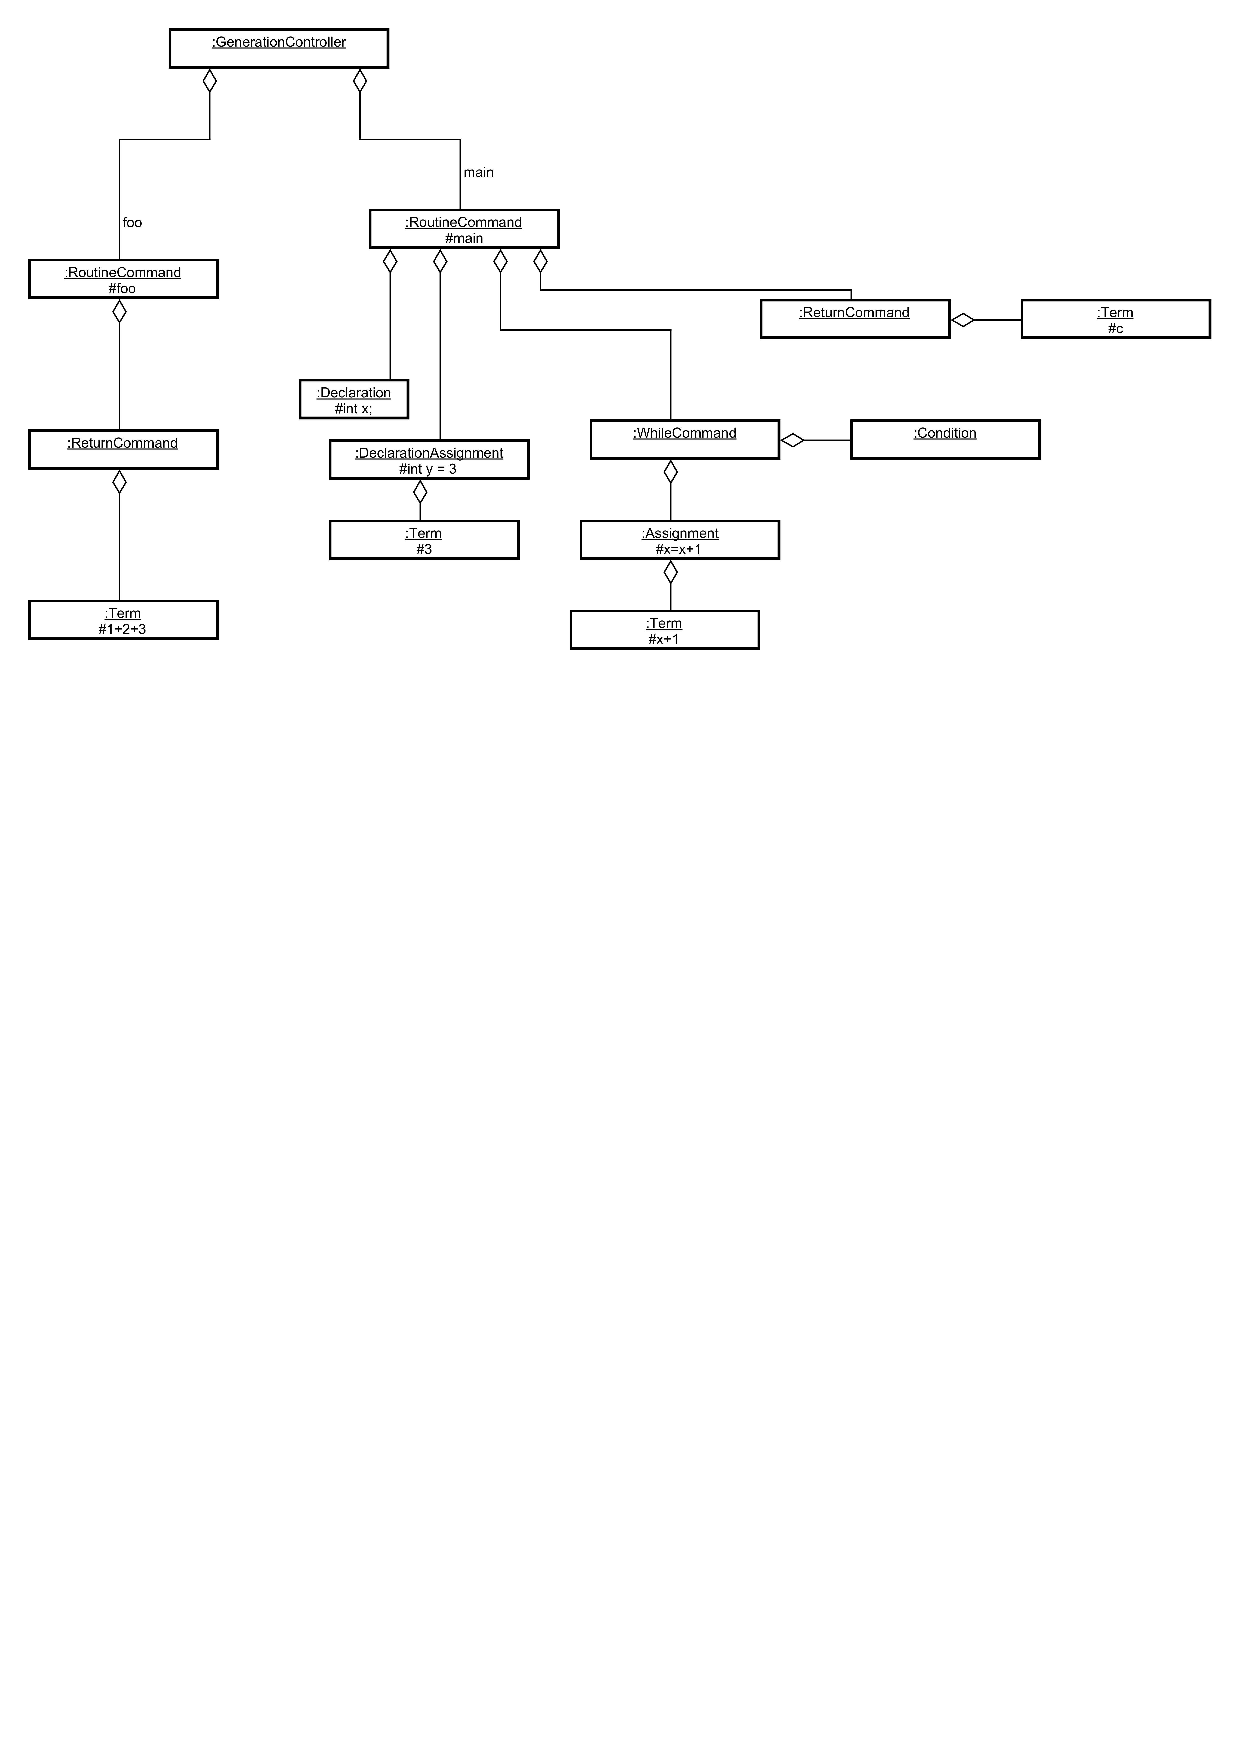
\includegraphics[width=1.2\textwidth]{diagrammIdeenUmlet/CommandTreeExample.pdf}}
\caption{Objektstruktur nach der Commanderzeugung}
\label{CommandTreeExample}
\end{figure}
Die tatsächliche Ausführung der Commands folgt dann: Der \textit{GenerationController} enthält einen Stack aus \textit{Scope}-Objekten. In diesen Objekten ist alles über die zum aktuellen Ausführungszeitpunkt vorhandenen Daten gespeichert, etwa die Datentypen oder Werte der Variablen. Zu Beginn legt der \textit{GenerationController} einen \enquote{Urscope} auf seinen Stack. Dieser enthält lediglich die Eingabevariablen. Dann wird die \textit{run()}-Methode des Wurzelbefehls des Befehlsbaums der Mainroutine ausgeführt. Jeder Befehl ändert dann entprechend seiner Semantik die Werte im aktuell obersten Scope auf dem Stack. Dabei muss auch jeder Befehl eine entsprechende Typprüfung durchführen. Ein \textit{IfCommand} beispielsweise prüft seine Bedingung und führt seine Kinderbefehle im Baum aus, falls die Bedingung wahr ist. \\
Einen Spezialfall stellen die \textit{RoutineCall}-Commands dar. Ein solcher Befehl muss sich beim \textit{GenerationController} den Wurzelbefehl der passenden Routine holen, diesem die Argumente in Form einer Liste von \textit{Term}-Objekten übergeben, und diesen dann ausführen. Anschließend muss er sich vom \textit{GenerationController} den Rückgabewert holen. Dieser Wurzelknoten ist ein Objekt der \textit{Command}-Subklasse \textit{RoutineCommmand}. Solche Commands müssen bei Ausführung zunächst die Argumente holen, dann einen neues \textit{Scope}-Objekt auf den Stack legen, dann alle Kinder ausführen und danach den Scope wieder weglegen. Hierbei muss im Falle einer Funktion auch geprüft werden, ob ein Rückgabewert vorhanden ist.\\
Einen weiteren Spezialfall stellen \textit{ReturnCommand}-Objekte dar. Sie müssen im \textit{GenerationController} den Rückgabewert setzen und diesem mitteilen, dass die Routine beendet ist. Die darauffolgenden Befehle erkennen dies vor ihrerer Ausfühurung und führen sich nicht weiter aus. \\
Insgesamt gibt jeder Befehl nach der \textit{run()}-Methode eine Liste von  \textit{TraceState}-Objekten zurück. So gibt ein \textit{IfCommand}-Objekt also eine leere Liste zurück, falls die Bedingung nicht erfüllt ist, und die Konkatenation aller TraceStatelisten seiner Kinder sonst. Ein \textit{WhileCommand}-Objekt gibt dementsprechend die Listen seiner Kinder in wiederholter Form zurück. Die gesamte Liste verpackt der \textit{GenerationController} zu einem \textit{Trace}-Objekt und gibt einen \textit{TraceIterator} zurück.

\newpage
\section{Abhängigkeitseinteilung mit Blick auf die Implementierung}
\label{implementierung}
%Mit Blick auf den Implementierungsplan: Aufteilung in Klassen/Pakete, die unabhängig voneinander implementiert und getestet werden können.
\subsection{Abhängigkeiten}
Das Paketdiagramm besagt, dass FileHandler und DebugLogic nicht voneinader abhängen.
Beide werden von der Control benutzt und müssen somit korrekt implementiert sein, bevor die Control richtig funktionieren kann. Weiter führt die Control Methoden der GUIFacade aus, ist aber nicht von derer Abhängig, da diese nicht relevant ist für eine funktionierende Control.
Die GUI hingegen ist stark von der Control abhängig und kann ohne diese keine korrekten Daten anzeigen.

%TODO Pakete der Debuglogic aktualisieren, da noch nicht fertig
\subsection{Implementierung}
Die Implementierung der Hauptpakete kann durch den von Fassaden geprägten Entwurf und dem MVC-Konzept gleichzeitig geschehen. Es ist jedoch sinnvoll das Exception Paket als erstes zu implementieren, um später keine Stellen im Quelltext suchen zu müssen, an denen Fehler auftreten können.
Weiter sollten die Unterpakete der DebugLogic entsprechend der Benutztrelation implementiert werden, also zuerst AntlrParser, Interpreter und zum Schluss der Debugger.
Dieses Problem besteht bei den Hauptpaketen nicht, da für die Kommunikation ausschließlich Fassaden benutzt werden. Diese können zur gleichzeitigen Implementierung der Pakete als Stummel pseudoerstellt werden, d.h. die Methoden sind leer und enthalten keine bzw. nur sehr wenig Funktionalität.\\
Der FileHandler stellt wiederum eine Ausnahme dar, da er mehrere Klassen zur Repräsentation und Interaktion zum Dateisystem bereitstellt.
Hierbei müssen die Klassen ConfigurationFile, PropertiesFile und LanguageFile gleichzeitig mit der FileHandlerFacade Klasse einsatzbereit sein.

\begin{center}
\makebox[\textwidth][c]{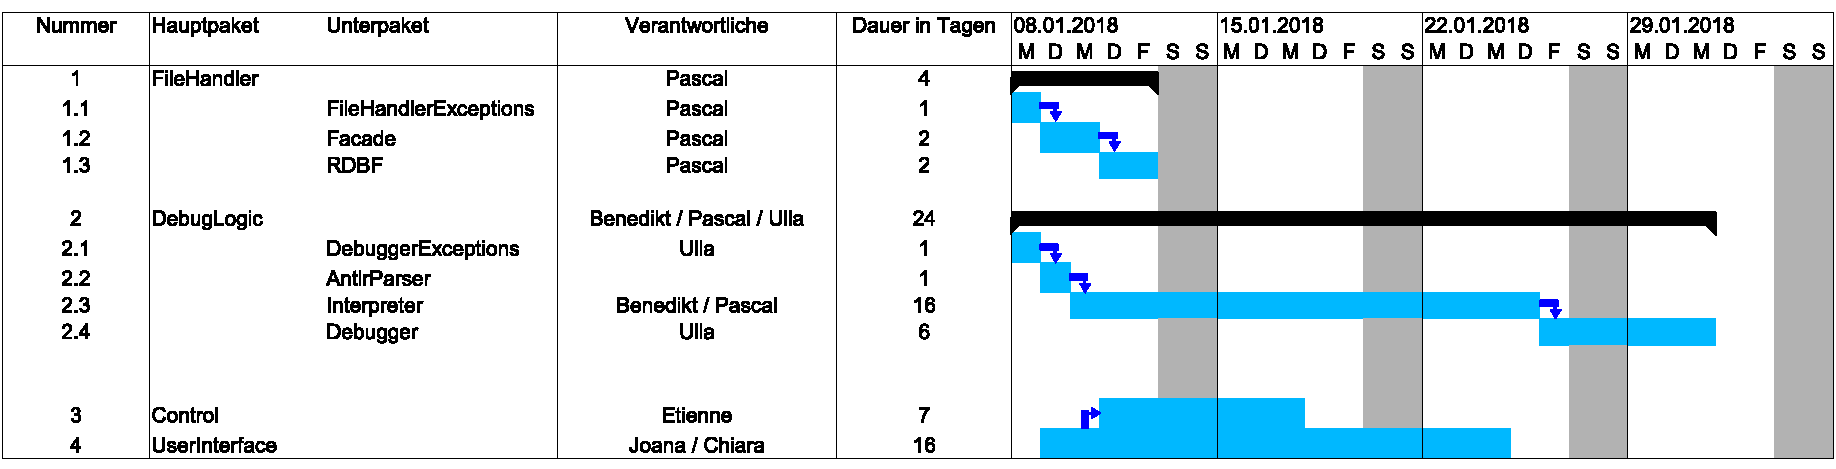
\includegraphics[width=1.15\textwidth]{GanttDiagramm_withArrows.pdf}}
\captionof{figure}{Gantt Diagramm: Zeitplanung der Implementierung}
\end{center}

\newpage
\section{Programmsprache, Antlr und Speicherformat}\label{FormSpez}

\subsection{Wlang}

Wlang ist eine prozedurale, imperative Sprache, welche weder objektorientiert, noch einrückungsbasiert ist. \\
Sie unterstützt die primitiven Datentypen int, long, float, double, char und boolean mit den selben Genauigkeiten wie Java.
Außerdem sind  bis zu dreidimensionale Arrays dieser Datentypen möglich. \\
Desweiteren unterstützt Wlang Kontrollstrukturen wie Funktionen und Prozeduren, die bedingten Ausführungen if, else if und else und while-Schleifen. \\
Es muss in jedem Programm eine main-Routine vorhanden sein, von der die Ausführung ausgeht. Routinen, die aufgerufen werden, müssen darüber stehen. Kommentare können
sowohl zeilenweise (//) als auch zeilenübergreifend (/*Kommentar*/) benutzt werden.
Sämtliche Variablen müssen innerhalb einer Routine stehen. Auch Rekursion ist möglich. \\
Für die Definition der Kontextfreien Antlr-Grammatik siehe Anhang, in den Unterkapiteln \ref{wlanggrammatik} und \ref{breakpointgrammatik}.


\subsection{Verwendung von Antlr}

Wie bereits im zweiten und dritten Kapitel beschrieben, benutzt der DIbugger im Paket \textit{DebugLogic.AntlrParser} extern erzeugte Java-Klassen, um die textuelle Nutzer-Eingabe zu einem ablaufbaren \textit{Parse Tree} umzuwandeln. Diese Klassen werden von dem frei verfügbaren Programm Antlr\textsuperscript{\textcopyright} (Version 4) erzeugt.
Ein \textit{Parse Tree} (manchmal auch \textit{Syntax Tree} genannt) ist dabei ein Baum mit einer eindeutigen Wurzel, der die syntaktische Struktur eines Textes – in diesem Fall der Nutzereingabe – mit Hilfe einer kontextfreien Grammatik darstellt. Die Spezifikation der Grammatik findet sich im Anhang, in den Unterkapiteln \ref{wlanggrammatik} und \ref{breakpointgrammatik}.

Auf Basis der Grammatik generiert Antlr mehrere Java-Klassen, wie einen Lexer, einen Parser, sowie einen Visitor und ein Visitor-Interface. Die Funktionalität dieser Klassen wird im Unterpaket \textit{DebugLogic.Interpreter} genutzt und erweitert.

\subsubsection{Vorteile der Verwendung eines Parser-Generators}
Die Verwendung eines Parser-Generators wie Antlr im Allgemeinen hat mehrere Vorteile gegenüber einem “von Hand” geschriebenen Parser: Offensichtlich spart es Zeit und Ressourcen, die in die Entwicklung des eigentlichen Produktes gesteckt werden können. Nicht zu vernachlässigen ist auch, dass Änderungen an der Grammatik zunächst nur in der Grammatik selbst gemacht werden müssen und nicht sofort Änderungen in mehreren, möglicherweise sehr großen Klassen nach sich ziehen. Zuletzt ermöglichen Parser-Generatoren wie Antlr, dass man ein Projekt auf einem Parser aufsetzt, der bereits von einer großen Gruppe an Nutzern getestet wurde, und so die Fehleranfälligkeit reduziert.


\subsubsection{Anforderungen an den verwendeten Parser-Generator}

Mindestanforderungen an einen Parser-Generator für dieses Projekt waren Java-Kompatibilität, Kostenfreiheit und eine offene Lizenz, die mit der vom DIbugger verwendeten Lizenz kompatibel ist.

Antlr kann Java-Code produzieren, ist kostenlos und unter BSD-Lizenz veröffentlicht.
Obwohl es auch andere Parser-Generator gibt, die diese Anforderungen erfüllen, spricht für Antlr, dass es auf allen Betriebssystemen läuft, in eine Entwicklungsumgebung eingebunden werden kann, eine aktuelle Version mit gutem Support bereitstellt und viele Online-Ressourcen dazu verfügbar sind.
Diese Faktoren erleichtern dabei nicht nur die gegenwärtige Entwicklung des Produkts sondern auch zukünftige Erweiterungen.

\subsection{Relational Debugger File (RDBF) Speicherformat}
RDBF ist ein nicht einrückungsbasiertes, imperatives Speicherformat, welches das Speichern von komplexen Blockstrukturen erlaubt.
Eine Blockstruktur besteht aus einem Blocknamen und Rumpf, welcher in sich wieder mehrere Blöcke und Daten hat.
Daten bestehen aus einem Namen, Wert und Typ, welcher aber erst von einem Parser herausgefunden werden muss.
Es werden die Datentypen String, int, long, float, double und boolean unterstützt.
Weiter gibt es einen spezialisierten TextBlock, der nur einen Fließtext zum Speichern enthält.
Kommentare können durch das Kennzeichnen am Anfang einer Zeile mit \enquote{//} erzeugt werden.
Das Speicherformat ist durch eine Kontextfreie Grammatik definiert. Diese kann im Anhang unter \ref{RDBF} eingesehen werden. 

\newpage
\section{Änderung zum Pflichtenheft}
\paragraph{Erweiterte Syntax für Watch-Expressions und bedinge Breakpoints}
In Kapitel 12.8 des Pflichtenheftes wurde die Syntax der Watch-Expressions und bedingter Breakpoints durch eine kontextfreie Grammatik definiert, welche zu den Funktionalen Anforderungen FA90 und FA110 gehört.
In dieser Grammatik war kein bedingter Breakpoint der Form $A\&\&B$ bzw. $A||B$ oder $!A$ ableitbar. Diese Einschränkung ergab sich als während des Entwurfs als nicht notwendig und wird demnach aufgehoben. Eine genaue Definition der Watch-Expressions und bedingten Breakpoints in Form einer Antlr-Grammatik ist im Anhang \ref{Anhang} zu finden. Insgesamt können diese auf syntaktischer Ebene aus beliebigen Termen bestehen. Dies ändert jedoch nichts an den Funktionalen Anforderungen FA90 und FA110, sondern nur an deren Umsetzung.



\newpage
\section{Anhang}
\label{Anhang}

Startnichtterminal in den Grammatiken ist immer die Variable \textit{r}.
\subsection{Kontextfreie Antlr-Grammatik für WLang-Syntax} \label{wlanggrammatik}
\begin{verbatim}

grammar Wlang;
r: programm;


programm: routine* mainRoutine;
routineHead: returntype = TYPE id = ID '(' args=arglist? ')' #FunctionHead
			| 'void' id =ID '('args=arglist?')' #ProcedureHead
			;

mainHead: returntype = TYPE 'main' '(' args=arglist? ')' #MainFunctionHead
			| 'void' 'main' '('args=arglist?')' #MainProcedureHead
			;

arglist: argument ',' arglist | argument;
argument: type=TYPE id=ID;
filledArglist: filledArgument ',' filledArglist | filledArgument;
filledArgument: term;
routine: routineHead block;
mainRoutine: mainHead block;

//Statements

statements : statement statements #CompStatement 
			| statement #SingleStatement
			;
statement:  ifState 
		| ifelseState 
		| whileState 
		| assignment
		| arrayDeclaration
		| arrayDeclareAssign
		| arrayElementAssign
		| declaration 
		| funcCall ';'	
		| returnState;
		

funcCall: functionname = ID '(' args=filledArglist? ')' 
	  |functionname = 'main' '(' args=filledArglist? ')'
	;

	
block: '{'statements'}';
assignment: declareAssign
			| pureAssign
			;

arrayDeclaration: type = TYPE dims id = ID ';';
arrayDeclareAssign: type = TYPE dims id = ID ASSIGN '{'filledArglist'};';
arrayElementAssign: arrayAccess ASSIGN value = term';';
dims: '['term']' #oneDims
	| '['term']''['term']' #twoDims
	| '['term']''['term']''['term']' #threeDims
	;


pureAssign: id = ID ASSIGN value = term ';';
declareAssign: type = TYPE id = ID ASSIGN value = term ';';
declaration: type = TYPE id = ID ';';
returnState: 'return' returnvalue = term ';';

//Kontrollstrukturen
ifState: 'if' '(' condition ')' block
	| 'if' '(' condition ')' statement
	;
ifelseState: ifState 'else' block
	| ifState 'else' statement
	;
whileState: 'while' '(' condition ')' block
	| 'while' '(' condition ')' statement
	;
//Bedingungen
condition: ID #IdCondition
	| arrayAccess #ArrayAccessCondition
	| comparison #ComparisonCondition
	| BOOLEANLITERAL #ConstantCondition
	| '('condition')'#BracketCondition
	| condition '&&' condition #AndCondition
	| condition '||' condition #OrCondition
	| '!'condition #NotCondition
	;

comparison: left=term '<' right=term #LessComp
	   | left=term '<=' right=term #LessEqualComp
	   | left=term '>' right=term #MoreComp
	   | left=term '>=' right=term #MoreEqualComp
	   | left=term '==' right=term #EqualComp
	   | left=term '!=' right=term #NotEqualComp
	;

term : '-' inner = term #NegativeTerm
    | left = term '/' right = term #Division
	| left = term '*' right = term #Multiplication
	| left = term '-' right = term #Subtraction
	| left = term '+' right = term #Addition
	| left = term '%' right = term #Modulo
	|'('term')' #Brackets
	| FLOATLITERAL #FloatLiteral
	| INTLITERAL #IntLiteral
	| LONGLITERAL #LongLiteral
	| DOUBLELITERAL #DoubleLiteral
	| ID #ID
	| CHARLITERAL #CharLiteral
	| funcCall #FunctionCallInTerm
	| arrayAccess #ArrayAccessInTerm
	;

arrayAccess: id = ID '['index=term']' #OneDimArrayAccess
		| id = ID '['firstIndex=term']' '['secondIndex=term']' #TwoDimArrayAccess
		| id = ID '['firstIndex=term']' '['secondtIndex=term']' '['thirdIndex=term']' #ThreeDimArrayAccess
		;


//LITERALE bzw TOKENS

COMPOPERATOR:  '<'|'>'|'<='|'>='|'=='|'!=';
WS : [ \t\r\n]+ -> skip ; // skip spaces, tabs, newlines
COMMENT:   '/*' .*? '*/' -> skip;
LINE_COMMENT:   '//' ~[\r\n]* -> skip;
TYPE: 'float' | 'int' | 'char' | 'boolean' | 'double' | 'long';
ID : ([a-z]|[A-Z])+ ;
INTLITERAL: '-'? [1-9][0-9]* | '0';
FLOATLITERAL: ([1-9][0-9]*'.'[0-9]+ | '0') 'f';
CHARLITERAL: '\'' ~['\\\r\n] '\'';
BOOLEANLITERAL:	'true'|	'false';
NULLLITERAL: 'null';
LONGLITERAL: ([1-9][0-9]* | '0' )'L';
DOUBLELITERAL: [1-9][0-9]*'.'[0-9]+ | '0';
ASSIGN: '=';
\end{verbatim}
\subsection{Kontextfreie Antlr-Grammatik für Syntax von bedingten Breakpoints und Watch-Expressions} \label{breakpointgrammatik}
\begin{verbatim}
grammar Terms;
r: generalTerm;

generalTerm: condition | term;

condition: ID #IdCondition
	| arrayAccess #ArrayAccessCondition
	| comparison #ComparisonCondition
	| BOOLEANLITERAL #ConstantCondition
	| '('condition')'#BracketCondition
	| condition '&&' condition #AndCondition
	| condition '||' condition #OrCondition
	| '!'condition #NotCondition
	;
	
//Bedingungen
comparison: left=term '<' right=term #LessComp
	   | left=term '<=' right=term #LessEqualComp
	   | left=term '>' right=term #MoreComp
	   | left=term '>=' right=term #MoreEqualComp
	   | left=term '==' right=term #EqualComp
	   | left=term '!=' right=term #NotEqualComp
	;

term : '-' inner = term #NegativeTerm
    | left = term '/' right = term #Division
	| left = term '*' right = term #Multiplication
	| left = term '-' right = term #Subtraction
	| left = term '+' right = term #Addition
	| left = term '%' right = term #Modulo
	|'('inner = term')' #Brackets
	| FLOATLITERAL #FloatLiteral
	| INTLITERAL #IntLiteral
	| LONGLITERAL #LongLiteral
	| DOUBLELITERAL #DoubleLiteral
	| ID #ID
	| CHARLITERAL #CharLiteral
	| arrayAccess #ArrayAccessInTerm
	;

arrayAccess: id = ID '['index=term']' #OneDimArrayAccess
		| id = ID '['firstIndex=term']' '['secondIndex=term']' #TwoDimArrayAccess
		| id = ID '['firstIndex=term']' '['secondtIndex=term']' '['thirdIndex=term']' #ThreeDimArrayAccess
		;

//LITERALE bzw TOKENS

COMPOPERATOR:  '<'|'>'|'<='|'>='|'==';
WS : [ \t\r\n]+ -> skip ; // skip spaces, tabs, newlines
COMMENT:   '/*' .*? '*/' -> skip;
LINE_COMMENT:   '//' ~[\r\n]* -> skip;
TYPE: 'float' | 'int' | 'char' | 'boolean';
ID : [A-Z]'.'([a-z]|[A-Z])+ ;
INTLITERAL: [1-9][0-9]* | '0';
FLOATLITERAL: ([1-9][0-9]*'.'[0-9]+ | '0') 'f';
CHARLITERAL: '\'' ~['\\\r\n] '\'';
BOOLEANLITERAL:	'true'|	'false';
NULLLITERAL: 'null';
LONGLITERAL: ([1-9][0-9]* | '0' )'L';
DOUBLELITERAL: [1-9][0-9]*'.'[0-9]+ | '0';
ASSIGN: '=';

\end{verbatim}

\subsection{Kontextfreie Grammatik RDBF Format} \label{RDBF}
\begin{verbatim}
R : ((STATEMENT | BLOCK | BLOCK_TEXT | COMMENT) NEWLINE)*;

BLOCK : VARIABLE '{' NEWLINE
	((STATEMENT | BLOCK | COMMENT) NEWLINE)*
	NEWLINE '}';
BLOCK_TEXT : VARIABLE '{' NEWLINE 'def_blockLen=' I_VALUE NEWLINE TEXT NEWLINE '}';
	
STATEMENT : VARIABLE '=' VALUE;

COMMENT : '//' (WORD SPACE?)*;

VALUE : (I_VALUE | L_VALUE | F_VALUE | D_VALUE | B_VALUE | S_VALUE);
I_VALUE : NUMBER+;
L_VALUE : NUMBER+ 'L';
F_VALUE : NUMBER+ ('.' NUMBER*)? 'f';
D_VALUE : NUMBER+ ('.' NUMBER*)?;
B_VALUE : 'true' | 'false';
S_VALUE : '\'' (WORD SPACE?)* '\'';

TEXT : ((~[])* (SPACE | NEWLINE)?)*;
WORD : (LITERAL | NUMBER | SPEC_CHAR)+;
VARIABLE : (LITERAL | NUMBER | SPEC_CHAR_VAR)+;

LITERAL : [A-Z] | [a-z];
NUMBER : [0-9];
SPEC_CHAR : ~('\'' | NEWLINE);
SPEC_CHAR_VAR : '$' | '&' | '_';
NEWLINE : '\n';
SPACE : ' ';
\end{verbatim}
\end{document}
\grid
\grid
\grid
